\documentclass[8pt]{article}

%%%%%%%%%%%%%%%%
%%% Packages %%%
%%%%%%%%%%%%%%%%

\usepackage[utf8]{inputenc}
\usepackage[english]{babel}
\usepackage{graphicx}
\usepackage{amsmath,amssymb,amsbsy,amsthm,color}
\usepackage{mathtools}
\usepackage[paperwidth=19cm,paperheight=29.7cm,hmargin=2cm,vmargin=3cm]{geometry}

\usepackage[square,numbers]{natbib}


\begin{document}

\bibliographystyle{natbib}
	
\title{\vspace{-2.2cm} Hamiltonian Saddle-Node Bifurcations \\ in Chemical Reaction Dynamics}

\date{}	
	
\maketitle

\vspace{-0.9cm}

\section{Introduction}

In this chapter we describe the influence of Hamiltonian saddle-node bifurcations on the high-dimensional phase space structures that mediate transport and characterize reaction dynamics \cite{GG2019}. We do so by identifying the relevant invariant manifolds, NHIMs and their stable and unstable manifolds, using the method of Lagrangian descriptors (LDs). In a general context, a saddle-node bifurcation takes place when a saddle and an elliptic equilibrium point of a dynamical system 'collide' as the value of a physical parameter is varied. This phenomenon occurs naturally in a Chemistry setup as a consequence of lowering the energy barrier height associated to a saddle point of a given potential energy surface (PES), which results in the connection of the potential well region on one side of the saddle to a escape channel. Therefore, this mechanism facilitates that trajectories cross the phase space bottleneck in the neighborhood of the index-1 saddle, and hence has a great influence on reaction dynamics. The drastic changes produced in the geometry of the phase space structures can then be used to account for corrections to Kramers' reaction rate as the barrier height decreases \cite{hathcock2019renormalization}, providing a significant step for the experimental study of single bond dynamics of molecules and the control of micro- and nano-electromechanical devices \cite{hathcock2019renormalization,husson2009force,miller2012escape,herbert2017predictability}. A nice example regarding the influence of Hamiltonian saddle-node bifurcations on isomerization dynamics can be found in that of the LiCN/LiNC molecule \cite{borondo1995,borondo1996,revuelta2019unveiling}. Other applications include the study of ionization and dissociation rates in atomic systems \cite{de_leon_intramolecular_1981,mitchell_geometry_2003_I,mitchell_geometry_2003_II,mitchell_chaos-induced_2004,mitchell_analysis_2004,mitchell_structure_2007,mitchell_nonlinear_2009,wang_photoionization_2010}. 

\smallskip

In the framework of chemical reaction dynamics, saddle-node bifurcations occur in problems that address the escape from a potential well by crossing an energy barrier and the influence that the barrier height has on the reactive flux. These situations can be identified for instance with dissociation or fragmentation reactions, where a chemical transformation takes place if the bond of a molecule A breaks up, giving rise to two products B and C. In this situation, the equilibrium conformation of the given molecule A is represented by a potential well in a PES, and dissociation into B and C can take place if the system has sufficient energy to croos the potential barrier that separates bounded (vibration) from unbounded (bond breakup) motion. This phenomenon can be modeled for instance by means of a cubic potential energy function as illustrated in Fig. \ref{fig:pes_snbif}, which will be our building block to construct the normal form Hamiltonian that describes saddle-node bifurcations in phase space. Our goal is to determine the geometrical phase space structures that ``divide'' reactants from products, and identify dynamically distinct phase space regions corresponding to reactive and non-reactive initial conditions for the dynamical system.

\begin{figure}[htbp]
	\begin{center}		
		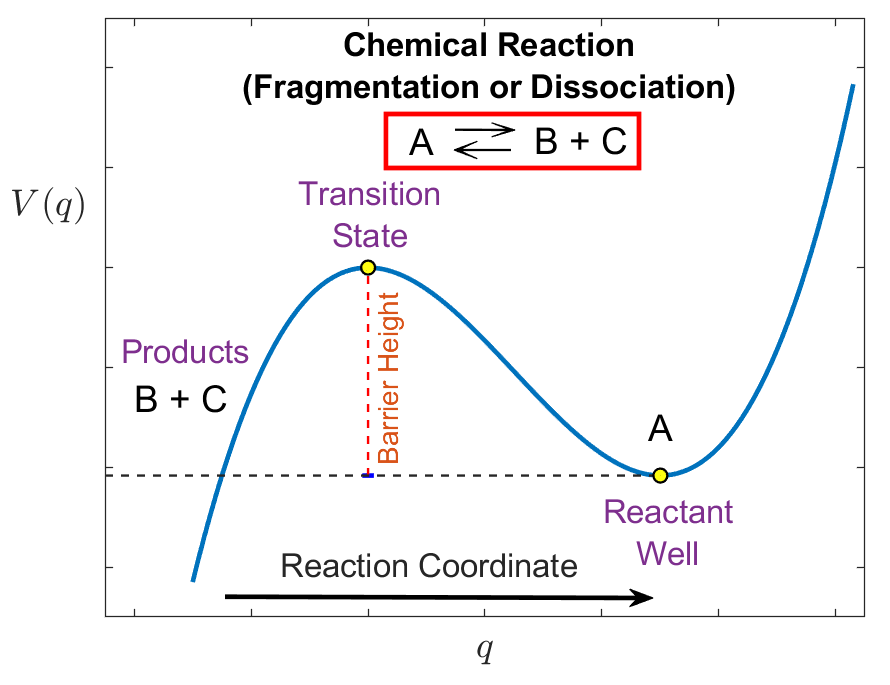
\includegraphics[scale=0.3]{fig1.png}
	\end{center}
	\caption{Cubic potential energy function as a basic model for dissociation chemical reactions. The shape of this potential is the building block (normal form) for Hamiltonian saddle-node bifurcations in phase space.}
	\label{fig:pes_snbif}
\end{figure}


\section{Hamiltonian Saddle-Node Bifurcation in 1-DoF Systems}

We begin our analysis by looking at the normal form Hamiltonian describing a saddle-node bifurcation in phase space for a system with one degree of freedom (DoF). The total energy of the system is defined in the classical way as the sum of kinetic plus potential energy in the form:
\begin{equation}
H(u,v) = \frac{1}{2} \, v^2  - \mu \, u + \frac{1}{3} \,u^3 \;,
\label{eq:ham_1dof}
\end{equation}
where the potential energy function is a cubic in the variable $u$ representing the DoF, and $\mu \in \mathbb{R}$ is the bifurcation parameter. Hamilton's equations of motion are given by:
\begin{equation}
\begin{cases}
\dot{u} = \dfrac{\partial H}{\partial v} = v \\[.3cm]
\dot{v} = -\dfrac{\partial H}{\partial u} = \mu - u^2
\end{cases},
\label{eq:hameq1}
\end{equation}
and the equilibrium points are located at $(u,v) = (\pm\sqrt{\mu},0)$. Notice that for $\mu > 0$ we have two different equilibria whcih approach each other as the bifurcation parameter goes to zero. At $\mu = 0$ both equilibria ``collide'' into one equilibrium point at the origin, and when $\mu < 0$ the resulting dynamical system has no equilibria. The linear stability of the equilibria is easily obtained by computing the eigenvalues of the Jacobian matrix at each equilibrium point. This yields:
\begin{equation}
J(u,v) = 
\begin{pmatrix*}[r]
\dfrac{\partial^2 H}{\partial u \partial v} & \dfrac{\partial^2 H}{\partial v^2} \, \\[.4cm]
-\dfrac{\partial^2 H}{\partial u^2} & -\dfrac{\partial^2 H}{\partial v \partial u} \,
\end{pmatrix*} = 
\begin{pmatrix}
0 & 1 \\
-2 u & 0
\end{pmatrix} \quad \Rightarrow \quad 
\begin{cases}
J(-\sqrt{\mu},0) = 
\begin{pmatrix}
0 & 1 \\
2 \sqrt{\mu} & 0
\end{pmatrix} \\[.5cm]
J(\sqrt{\mu},0) = 
\begin{pmatrix}
0 & 1 \\
-2 \sqrt{\mu} & 0
\end{pmatrix}
\end{cases}
\end{equation}
and, whenever the bifurcation parameter is positive, $(-\sqrt{\mu},0)$ is a saddle since the eigenvalues are $\pm \sqrt[4]{4\mu}$, and $(\sqrt{\mu},0)$ is a center because the eigenvalues are pure imaginary $\pm \sqrt[4]{4\mu} \, i$. For $\mu = 0$, the only eigenvalue of the Jacobian matrix is zero, and thus the linearization does not provide enough information, and one needs to include higher order terms to determine the stability of the equilibrium point $(0,0)$.

\smallskip

In Fig.~\ref{fig:ld_bif_sn} we illustrate how the method of Lagrangian descriptors detect the invariant manifolds and the saddle-node bifurcation in the phase portrait of the dynamical system given in Eq. \eqref{eq:hameq1}. Since in this cubic potential trajectories can escape off to infinity in finite time depending on the total energy of the system and the location of the initial conditions, we have applied variable integration time LDs to avoid this issue. In particular, we have used the $p$-norm definition of LDs with exponent $p = 1/2$ and the intergation time considered for trajectories is $\tau = 8$ as they evolve forward and backward. Furthermore, whenever a trajectory leaves the domain defined by the circle of a certain radius about the origin, we stop the numerical integration of that trajectory. Notice how the stable and unstable manifolds are highlighted by the singularities present in the LD scalar field. Moreover, it is interesting to highlight from Fig. \ref{fig:ld_bif_sn} D) that at the critical bifurcation value $\mu = 0$, the values attained by LDs in the neighborhood of the origin seem to indicate that a bifurcation in the phase space structure is going to take place. Notice that a `ghost' center structure is about to be created close to the cusp at the origin.

\begin{figure}[htbp]
	\begin{center}
		A)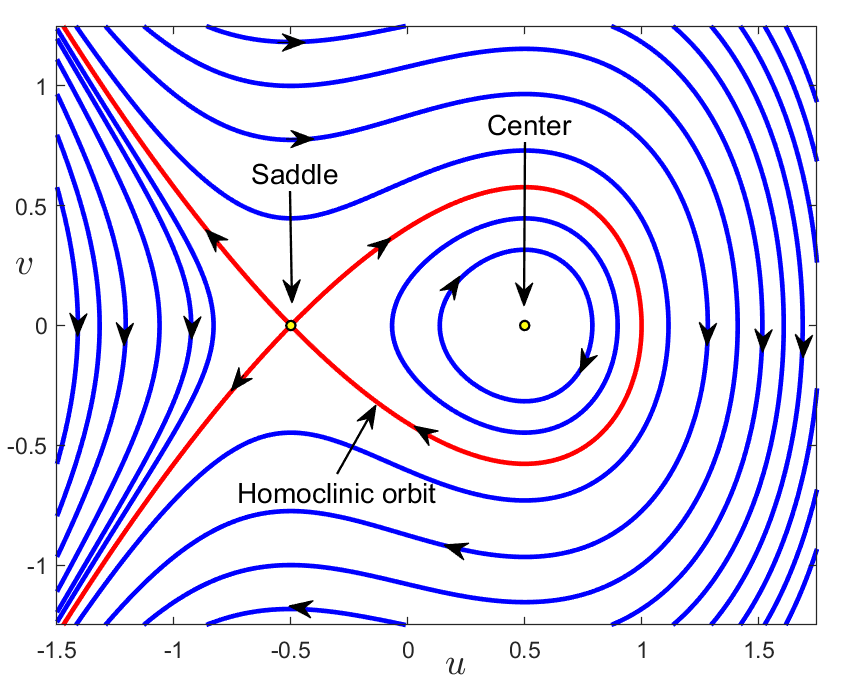
\includegraphics[scale=0.26]{fig2a.png}
		B)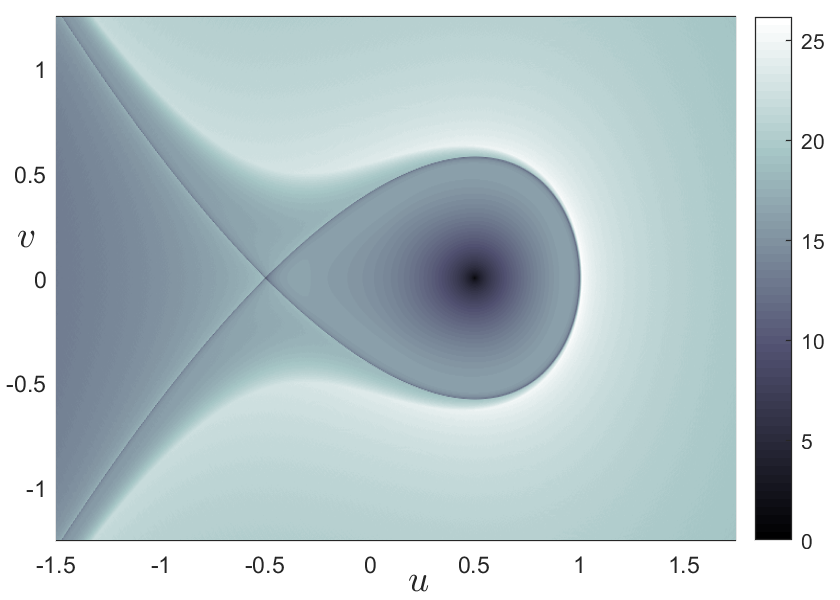
\includegraphics[scale=0.3]{fig2b.png}
		C)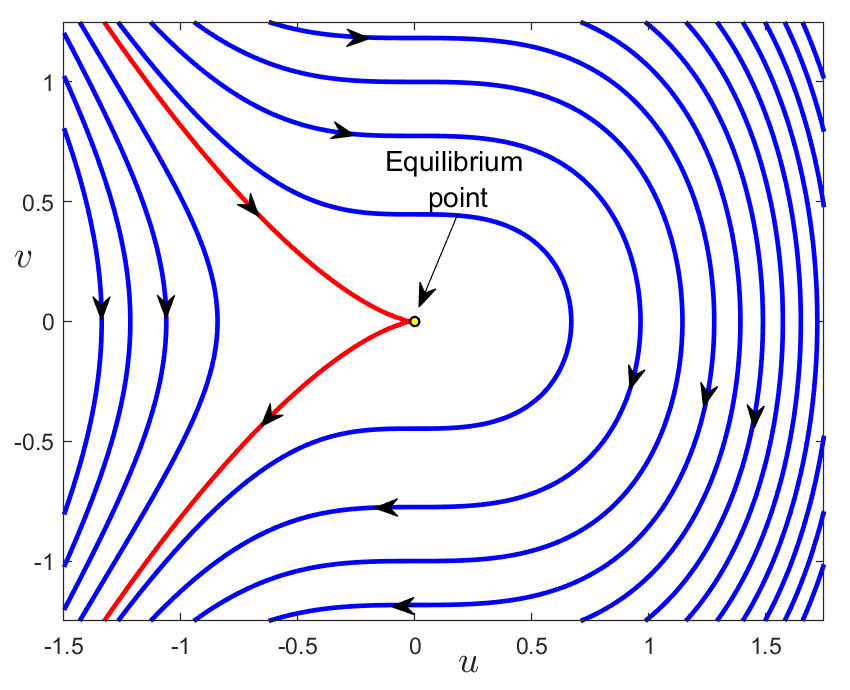
\includegraphics[scale=0.26]{fig2c.png}
		D)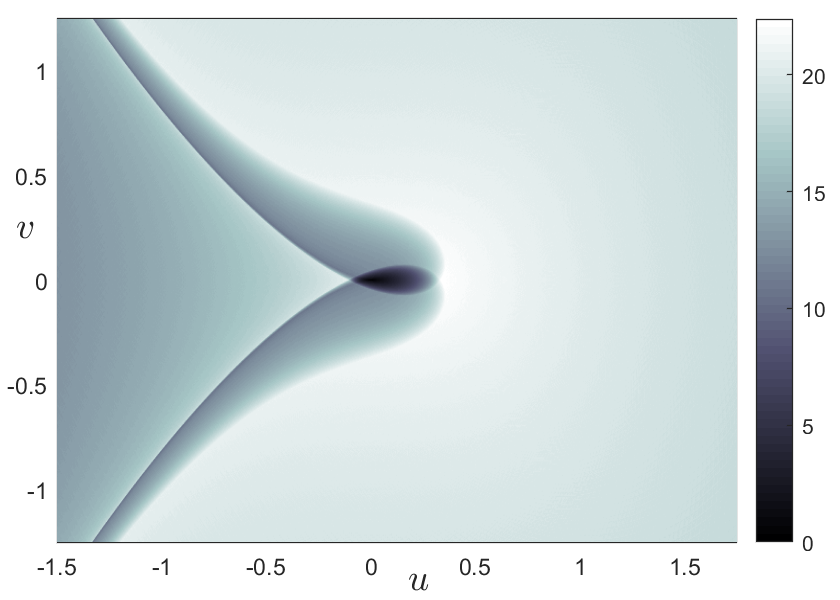
\includegraphics[scale=0.3]{fig2d.png}
		E)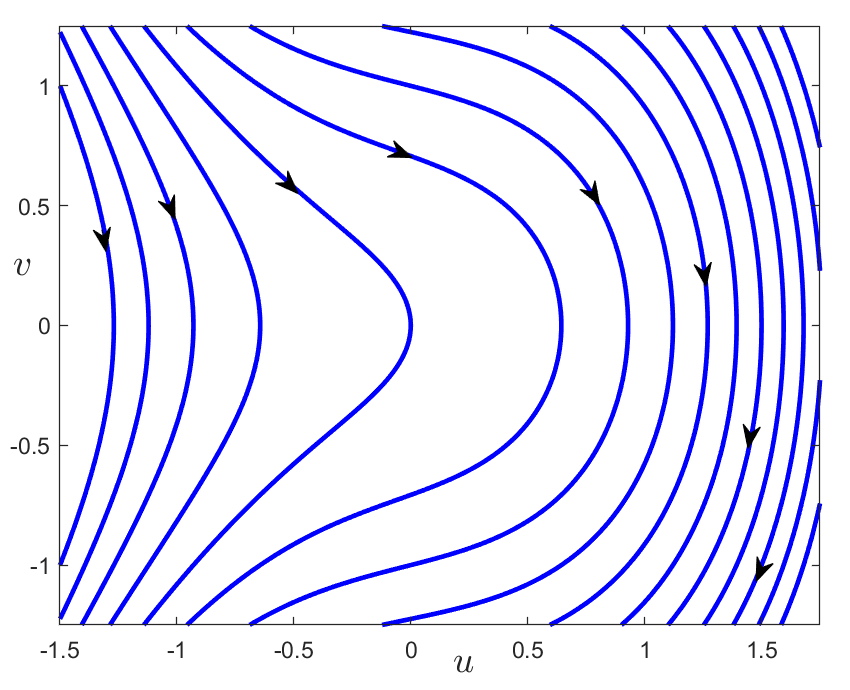
\includegraphics[scale=0.26]{fig2e.png}
		F)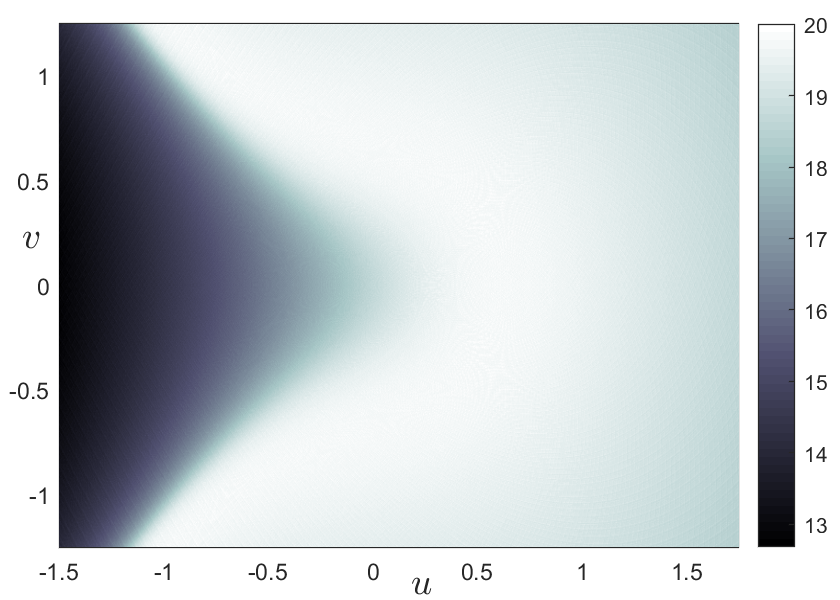
\includegraphics[scale=0.3]{fig2f.png}
	\end{center}
	\caption{Phase space portrait of the dynamical system in Eq. \eqref{eq:hameq1} (left column) and variable time LDs (right column). A) and B) correspond to $\mu = 0.25$; C) and D) $\mu = 0$; D) and E) $\mu = -0.25$. Trajectories are marked in blue, invariant manifolds in red, and equilibrium points as yellow dots.}
	\label{fig:ld_bif_sn}
\end{figure}

\smallskip

The next step that we take is to make the normal form Hamiltonian is Eq. \eqref{eq:ham_1dof} more general by fixing the saddle point at the origin. The purpose of this modification is to avoid that both equilibria move as the bifurcation parameter is varied, which will simplify considerably our later analysis of the implications of saddle-node bifurcations for chemical reaction dynamics. Let us consider the linear change of coordinates:
\begin{equation}
\begin{cases}
u = q - \sqrt{\mu} \\[.1cm]
v = p
\end{cases}
\; , \quad \mu \in \mathbb{R}^{+} \cup \lbrace0\rbrace .
\end{equation}
This transformation yields the dynamical system and associatd Hamiltonian in the new coordinates:
\begin{equation}
\begin{cases}
\dot{q} = p \\[.1cm]
\dot{p} = 2  \sqrt{\mu} \, q - q^2
\end{cases}
\quad \Leftrightarrow \quad H(q,p) = \frac{1}{2} \, p^2 - \sqrt{\mu} \, q^2 + \frac{1}{3} \, q^3
\label{eq:hameq2}
\end{equation}
where the saddle is now at the origin for all positive values of $\mu$, and the center is at $(2\sqrt{\mu},0)$. In Fig. \ref{fig:ld_bif_sn_transf} we show the variable integration time LD using $\tau = 8$ for the Hamiltonian system in Eq. \eqref{eq:hameq2} with $\mu = 0.25$. We demonstrate how the stable and unstable manifolds of the saddle equilibrium point are identified at points where the LD scalar field is non-differentiable. The singular features can be easily visualized by taking one dimensional slices of the LD contour map, and jump discontinuities mark the initial conditions on an invariant manifold.

\begin{figure}[htbp]
	\begin{center}
		A)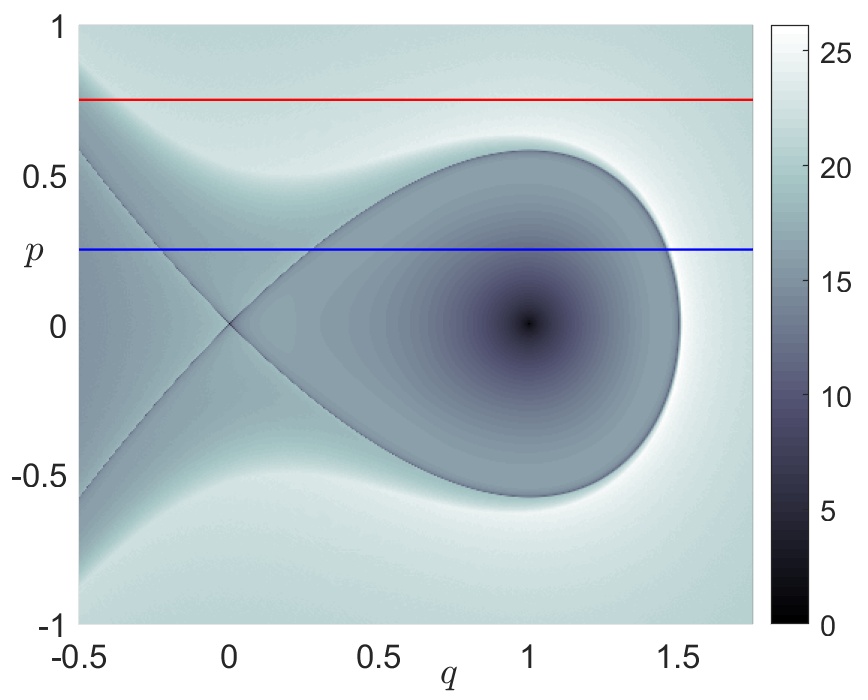
\includegraphics[scale=0.26]{fig3a.png}
		B)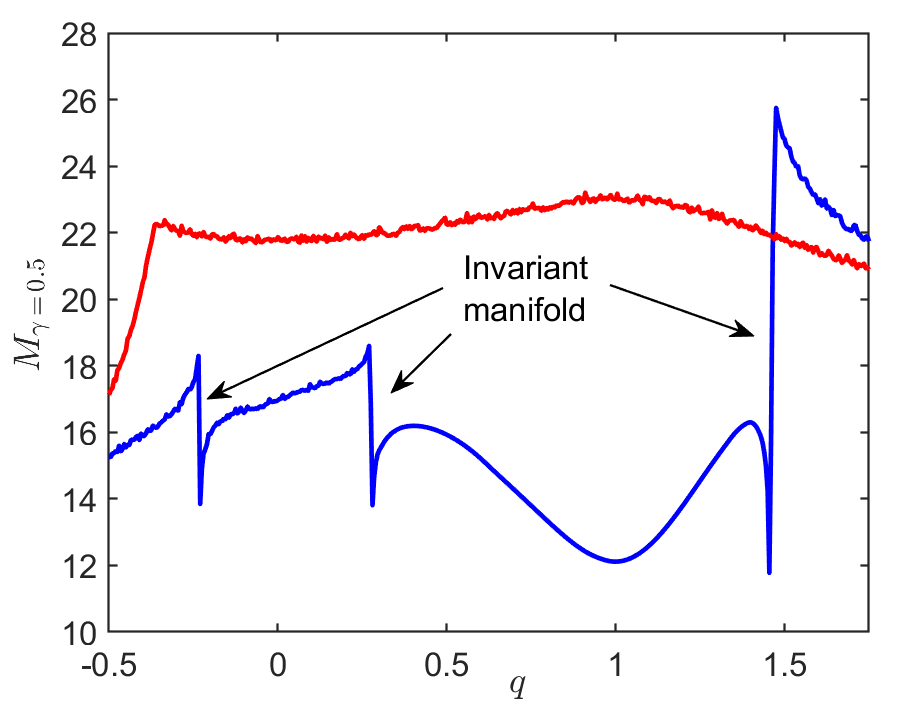
\includegraphics[scale=0.25]{fig3b.png}
	\end{center}
	\caption{A) Variable integration time LDs using $\tau = 8$ for the dynamical system in Eq. \eqref{eq:hameq2} for $\mu = 0.25$. B) Value of LDs along the lines of initial conditions $p = 0.25$ and $p = 0.75$ showing the location of manifolds at points where the LD scalar field in non-differentiable.}
	\label{fig:ld_bif_sn_transf}
\end{figure}

\smallskip

With the goal of controlling the potential well depth, we modify the cubic term that appears in the Hamiltonian of Eq. \eqref{eq:hameq2}. by introducing a parameter, $\alpha \in \mathbb{R}^{+}$, that allows us to vary the amplitude of this term, and consequently the strength of the nonlinearity. Thus, the Hamiltonian and Hamilton's equations become:
\begin{equation}
H(q,p) = \frac{1}{2} \, p^2 - \sqrt{\mu} \, q^2 + \frac{\alpha}{3} \, q^3 \quad \Leftrightarrow \quad \begin{cases}
\dot{q} = \dfrac{\partial H}{\partial p} = p \\[.4cm]
\dot{p} = -\dfrac{\partial H}{\partial q} = 2\sqrt{\mu} \, q - \alpha \, q^2
\end{cases} \;,
\label{eq:hameq_1dof_gen}
\end{equation}
where the potential energy function is:
\begin{equation}
V(q) =  - \sqrt{\mu} \, q^2 + \dfrac{\alpha}{3} \, q^3
\label{eq:pot_gen1D}
\end{equation} 
The dynamical system in Eq. \eqref{eq:hameq_1dof_gen} has a saddle equilibrum at the origin and a center at  $\left(2\sqrt{\mu}/ \alpha,0\right)$, and the Jacobian of the vector field is given by:
\begin{equation}
J(q,p) = 
\begin{pmatrix}
0 & 1 \\
2 \sqrt{\mu} -2 \alpha q & 0
\end{pmatrix}.
\end{equation}
The eigenvalues of the Jacobian at the equilibrium point $(0,0)$ are $\pm \sqrt[4]{4\mu}$ with corresponding eigenvectors $(1,\pm \sqrt[4]{4\mu})$, and the eigenvalues at the center equilibrium are $\pm \sqrt[4]{4\mu} \, i$ with eigenvectors $(1,\pm \sqrt[4]{4\mu} \, i)$. Observe that the eigenvalues and eigenvectors of the Jacobian evaluated at the equilibrium points do not depend on the well depth parameter $\alpha$. We determine well depth (or ``flatness'' $\mathcal{F}$) as the difference between the potential energy at the center (minimum of the well) and that of the saddle equilibrium:
\begin{equation}
\mathcal{F} = V\left(\frac{2\sqrt{\mu}}{\alpha}\right) - V(0)= \frac{4 \sqrt{\mu^3}}{3 \, \alpha^2} = \dfrac{\sqrt{\mu}}{3} \mathcal{D}^2 \; ,
\end{equation}
where $\mathcal{D} = 2\sqrt{\mu} / \alpha$ is the distance between the saddle and the center equilibrium point. Hence, for a fixed $\mu$, the well-depth increases as $\alpha$ gets smaller. Moreover, as $\alpha$ increases the well-depth approaches zero faster than the distance between the saddle and the center equlibrium points. In fact, the rate at which the well-depth changes with the distance between equilibria is given by:
\begin{equation}
\dfrac{d \mathcal{F}}{d \mathcal{D}} = \dfrac{2\sqrt{\mu}}{3} \mathcal{D} = \frac{1}{3} \lambda_0^2 \, \mathcal{D} \; .
\end{equation}
which is proportional to the product of the square of the eigefrequency (square of eigenvalues) associated to the saddle and the distance between equilibria. In Fig. \ref{fig:pes_1dof_alpha} A) we illustrate for a fixed value $\mu = 1$ how the well-depth and the distance between the saddle and the center equilibria change as the nonlinearity parameter $\alpha$ is varied.

\begin{figure}[htbp]
	\begin{center}
		A)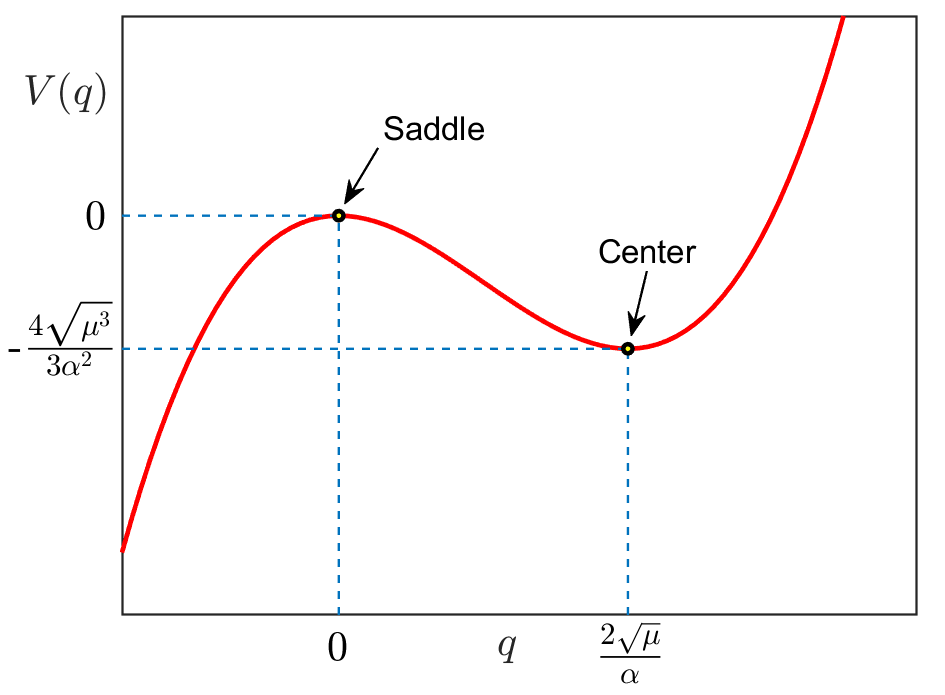
\includegraphics[scale=0.265]{fig4a}
		B)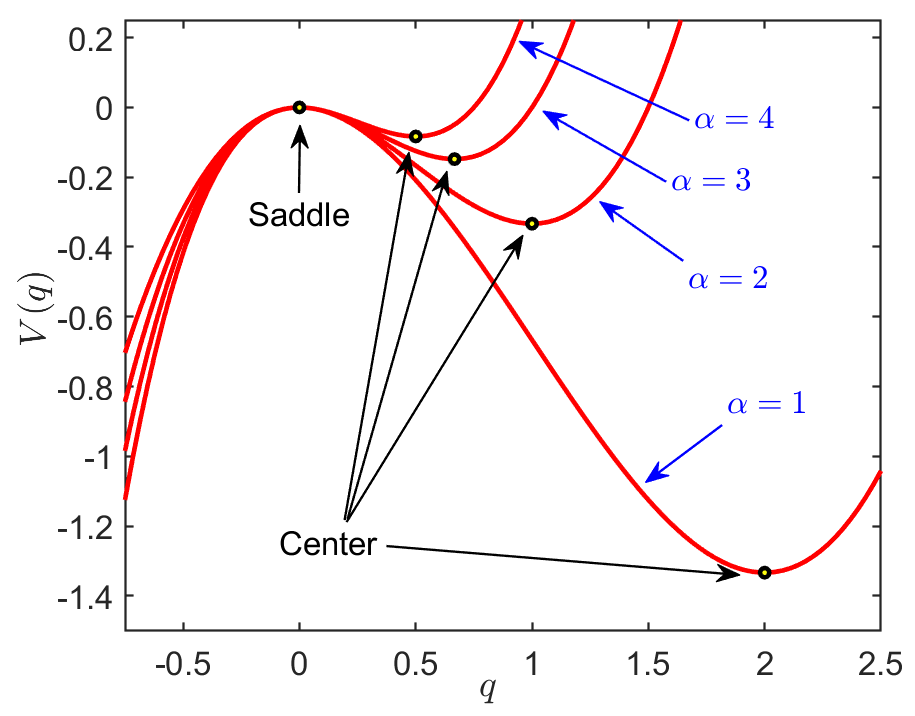
\includegraphics[scale=0.26]{fig4b} \\[.3cm]
		C)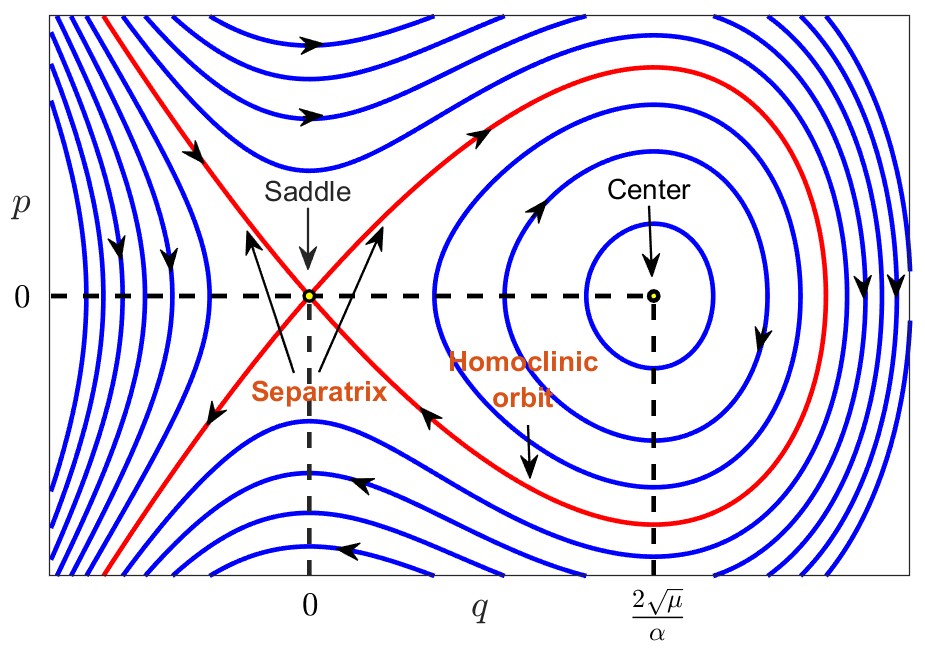
\includegraphics[scale=0.28]{fig4c}
	\end{center}
	\caption{A) Potential energy function described by Eq. \eqref{eq:hameq_1dof_gen} illustrating the depth parameter together with the horizontal distance from the saddle to the center equilibrium. B) Evolution of the potential energy function for a fixed value of $\mu = 1$ as $\alpha$ is varied. C) Phase portrait associated to the dynamical system in Eq. \eqref{eq:hameq_1dof_gen}.}
	\label{fig:pes_1dof_alpha}
\end{figure} 

We are now ready to discuss the phase space dynamics of the 1 DoF Hamiltonian in Eq. \eqref{eq:hameq_1dof_gen} and its implications for chemical reaction dynamics. First, we define what we mean by \textit{reaction} in this model. We say that reaction occurs when the configuration coordinate $q$ of a trajectory of the Hamiltonian system changes sign as it evolves in time. In particular, the trajectory crosses the energy barrier at the origin and escapes the potential energy well if $q$ goes from positive to negative. Recall that at the origin we have a saddle of the PES ad its energy is $H(0,0) = H_c = 0$, which we call the \textit{critical energy}. Moreover, the energy of the center equilibrium at the  bottom of the potential well is $H(2\sqrt{\mu}/\alpha,0) = H_w = - 4 \sqrt{\mu^3}/(3 \alpha^2)$. The phase space of the dynamical system in Eq. \eqref{eq:hameq_1dof_gen} is two-dimensional, and since total energy is conserved, trajectories evolve on the one-dimensional constant energy lines or isoenergetic contours of the Hamiltonian in the 2D phase space. Therefore, the system is completely integrable, and for a fixed energy $H_0$, trajectories evolve on the one-dimensional curve:
\begin{equation}
H_0 = \frac{1}{2} \, p^2 - \sqrt{\mu} \, q^2 + \frac{\alpha}{3} q^3
\end{equation}
We discuss the nature of the trajectories depending on the energy $H_0$ of the system:
\begin{itemize}
	\item \underline{\textbf{Energy Level $H_0 < H_w$:}} Consider an initial condition $\mathbf{x}_0 = (q_0,p_0)$ whose configuration coordinate satisfies $q_0 < q^{\ast}$, where $V(q^{\ast}) = H_0$, and the conjugate momentum is $p_0 \geq 0$. These points lie to the left of the potential energy barrier at the origin, and trajectories initially climb the potential energy landscape up to a point, where their velocity reverses direction and they roll down the potential hill escaping to infinity. Consequently, these trajectories cannot cross the barrier, since the saddle region is energetically forbidden, and we can classify them as nonreactive. We show them as blue curves in Fig. \ref{fig:dynbeh_1DoF}.
	
	\item \underline{\textbf{Energy Level $H_w \leq H_0 < H_c$:}} In this case, the equation $V(q) = 0$ has three roots, $q_1 < 0$ and $0 < q_2 < q_3$, and two types of trajectories are possible. For the initial conditions that satisfy $q_0 < q_1$, trajectories will behave similarly to the previous case. On the other hand, if initial conditions satisfy $q_2 < q_0 < q_3$, then the trajectory is forever confined to the potential well on the right of the potential barrier, since they are bounded by the homoclinic orbit. Threfore, they do not lead to reaction and are represented as green curves in Fig. \ref{fig:dynbeh_1DoF}. 
	
	\item \underline{\textbf{Energy Level $H_0 = H_c = 0$:}} When the total energy is equal to that of the barrier at the origin, the resulting trajectories approach the barrier asymptotically in forward and backward time. The initial conditions that start on the left of the potential barrier and asymptotically approach it in forward and backward time form pieces of the stable and unstable manifolds of the saddle equilibrium point. Furthermore, trajectories that start on the right of the potential barrier also approach the barrier as time goes to infinity, since they belong to the homoclinic orbit. All these trajectories are depicted as  black curves in Fig. \ref{fig:dynbeh_1DoF}.  
	
	\item \underline{\textbf{Energy Level $H_0 > H_c$:}} The energy of the system is above that of the barrier, and hence trajectories can escape from the well and lead to reaction. Therefore, the configuration space coordinate $q$ can change sign, and thus we define the dividing surface as $q = 0$. Trajectories must cross this surface   when escaping from the potential well and has the local non-recrossing property \cite{wiggins2016}. The isoenergetic dividing surface is given by: 
	\begin{equation}
	\mathcal{D} = \left\lbrace (q, p) \in \mathbb{R}^2 \; | \; q = 0 \;,\; \frac{p^2}{2}  = H_0 > 0  \right\rbrace = \left\lbrace \left(0, \pm \sqrt{2H_0}\right) \right\rbrace \;. \label{eq:snham_1dof_ds}
	\end{equation}
	We note that this dividing surface consists of two points and partitions the phase portrait into ``reactant'' and ```product'' regions. To characterize reaction dynamics, we note that the origin is a saddle equilibrium, and thus it is a NHIM, since dynamics is hyperbolic in directions normal to it \cite{wig2016}. Furthermore, recall that the linear stability of the saddle only depends on the $\mu$ parameter, due to the nature of the eigenvalues of the Jacobian. The eigenvectors are tangent to the stable and unstable manifolds at the origin, and can be used to numerically globalize the linear approximation. However, we can compute the stable and unstable manifolds of the saddle equilibrium analytically by noting that they lie on the zero level curve of the Hamiltonian:
	\begin{equation}
	\mathcal{W}^s(0,0) = \Gamma \cup \mathcal{W}^s_l(0,0) \;,\; \; \mathcal{W}^u(0,0) = \Gamma \cup \mathcal{W}^u_l(0,0) \;,
	\end{equation}
	where $\Gamma$ is the homoclinic orbit:
	\begin{equation}
	\Gamma = \left\lbrace  (q,p) \in \mathbb{R}^2 \; | \; q > 0 \;,\; H(q,p) = 0  \right\rbrace \;,
	\end{equation}
	and the left branches of the stable and unstable manifolds are:
	\begin{equation}
	\begin{split}
	\mathcal{W}^s_l(0,0) &= \left\lbrace  (q,p) \in \mathbb{R}^2 \; | \; q < 0 \:,\; p > 0 \;,\; H(q,p) = 0 \right\rbrace \\
	\mathcal{W}^u_l(0,0) &= \left\lbrace  (q,p) \in \mathbb{R}^2 \; | \; q < 0 \:,\; p < 0 \;,\; H(q,p) = 0 \right\rbrace
	\end{split} \;.
	\end{equation}
	We note here that the invariant manifolds are one-dimensional curves in $\mathbb{R}^2$, and form an impenetrable barrier between the reactive and nonreactive trajectories as shown in Fig. \ref{fig:dynbeh_1DoF}.
\end{itemize}



\begin{figure}[htbp]
	\begin{center}
		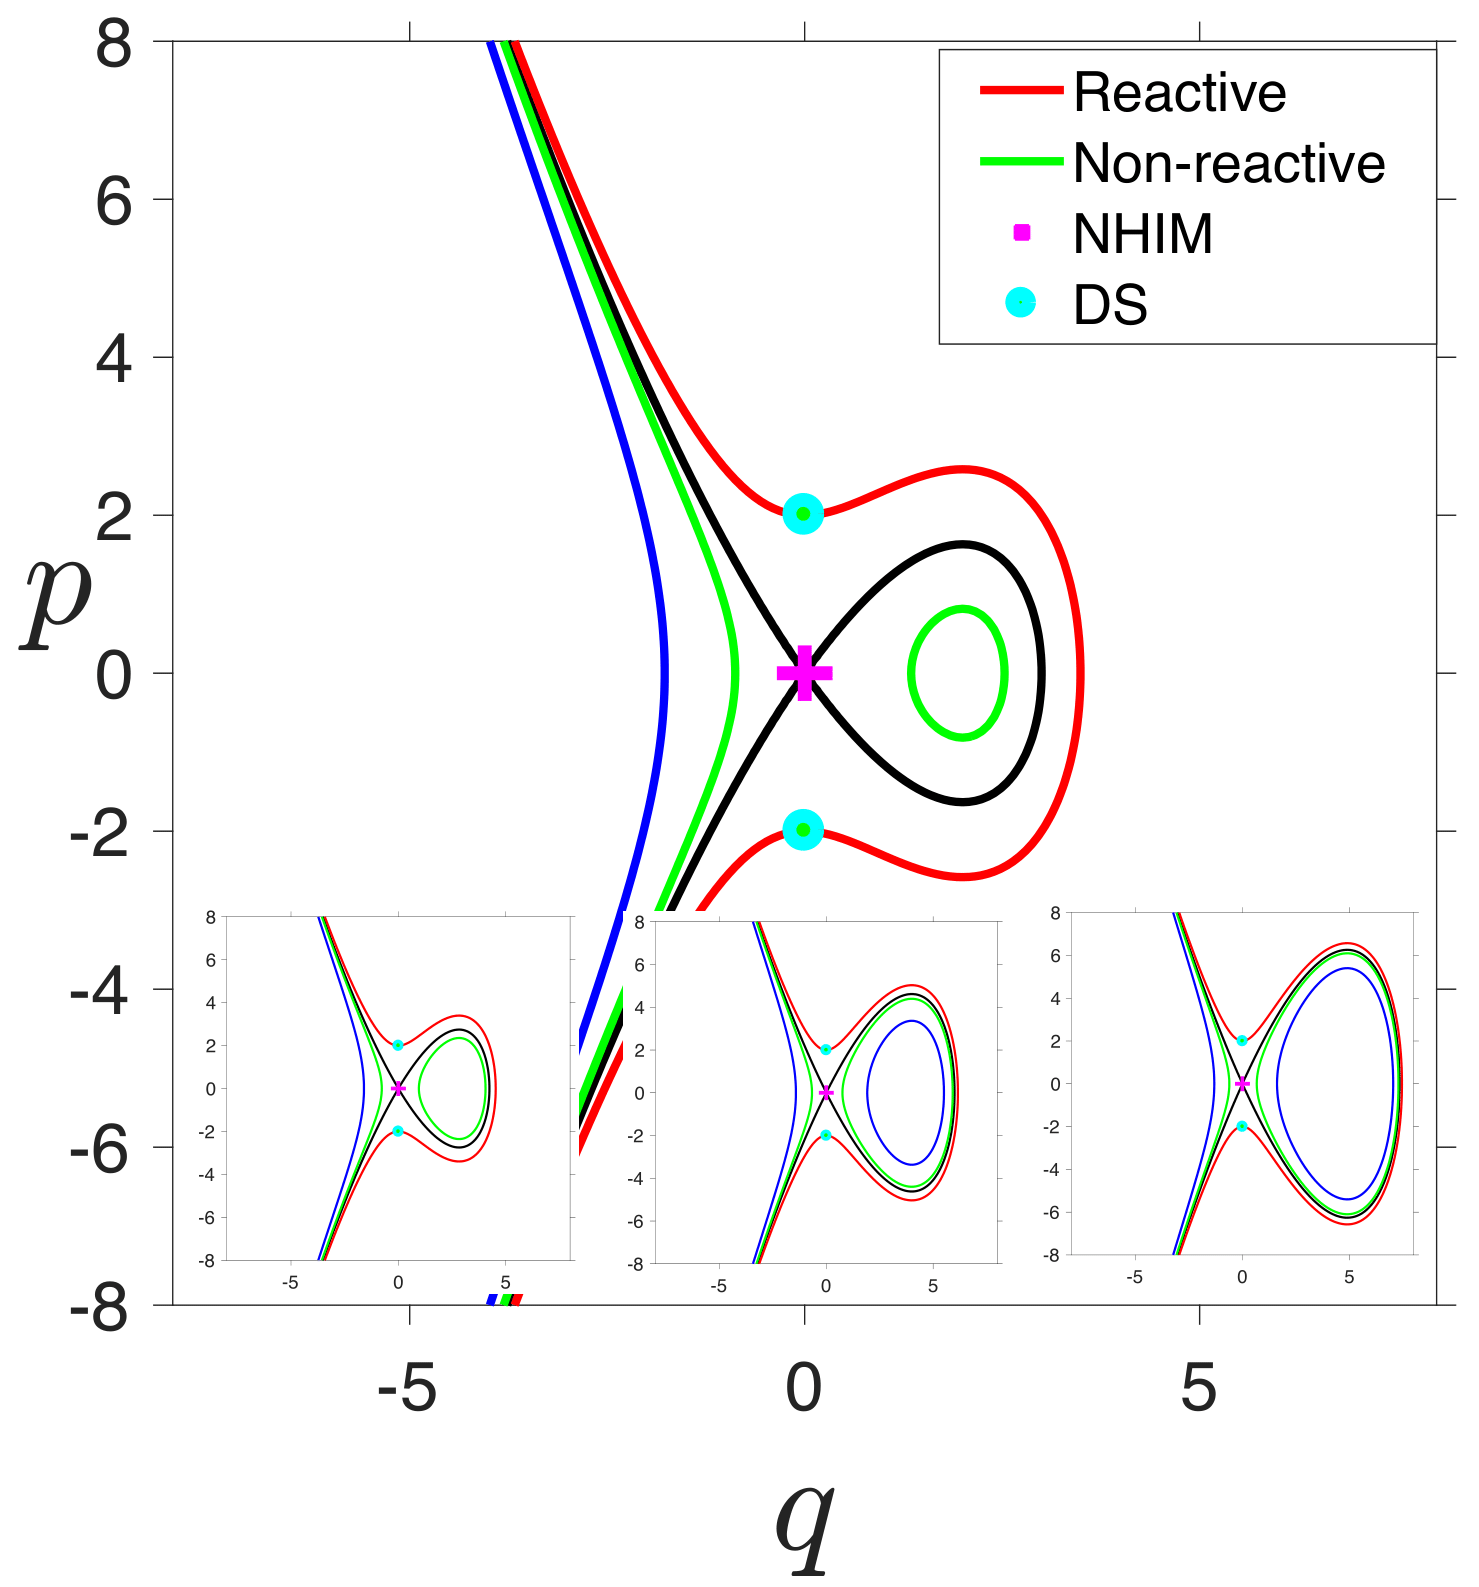
\includegraphics[scale=0.11]{fig5.png}
	\end{center}
	\caption{Trajectory behavior in the phase space of the Hamiltonian system in Eq. \eqref{eq:hameq_1dof_gen} for the model parameters $\mu = 1$ and $\alpha = 1$, with the insets $\mu = 2,\, 4, \, 6$. We show reactive (red) and nonreactive (blue) trajectories partitioned by the homoclinic orbit (black) formed by the unstable and stable manifolds of the NHIM at the origin (magenta cross). The reactive trajectory is at energy $H_0 = 2$, while the two nonreactive trajectories have energies $H_0 = -1, \, -5$. The dividing surface that the reactive trajectory must cross for reaction to occur is marked by cyan circles.}
	\label{fig:dynbeh_1DoF}
\end{figure}



%%%%%%%%%%%%%%%%%%%%%%%%%%%%%%%%%%%%%%%%%%%%%%%%%%%%%%%%%%%%%%%%%%%%%%%%%%%%%
%%%%%%%%%%%%%%%%%%%%%%%%%%%%%%%%%%%%%%%%%%%%%%%%%%%%%%%%%%%%%%%%%%%%%%%%%%%%%
%%%%%%%%%%%%%%%%%%%%%%%%%%%%%%%%%%%%%%%%%%%%%%%%%%%%%%%%%%%%%%%%%%%%%%%%%%%%%

%Our objective is to describe the change in a bond that signals the occurrence of a chemical reaction in terms of a unique characteristic of a trajectory of Hamilton's equations. This characteristic requires an understanding of the geometry of the phase space of the molecule in a way that enables us to divide an appropriate volume of phase space into a region corresponding to ``reactants'' and a region corresponding to ``products''. The passage from reactants to products, that is ``reaction'', occurs when a trajectory crosses the ``dividing surface'' (DS) between the reactants and products. In this framework for understanding chemical reactions, the flux through such a dividing surface would be related to the reaction rate, and therefore the construction of DS between such regions is of interest in reaction dynamics. The description of the regions of reactants and products can often be inferred from the nature of the development of the coordinates used in the mathematical model of the chemical reaction. Once the model is developed, the DS must be constructed in the context of this model. In relating the flux through the DS to a reaction rate it is desirable that trajectories crossing the DS from the reactant side proceed to the product side before possible recrossing the DS back to the reactant region. Thus, we require the DS to have the ``no-recrossing'' property\cite{MacKay90, waalkens2004direct}.  Hamiltonian dynamics conserves energy and therefore the trajectories evolve on a fixed energy surface of one less dimension (referred to as {\it codimension one}) than the phase space. The DS is required to be codimension one in the energy surface. Hence, we require a DS between reactants and products to be codimension one in the energy surface and to have the no-recrossing property. We note that Wigner had already described these properties for a DS in phase space much earlier\cite{Wigner38, Wigner39}, and a review of classical and quantum versions of DS constructed in phase space can be found in \cite{WaalkensSchubertWiggins08}. 
%
%Traditionally, the construction of DS was initially focused on critical points of the potential energy surface (PES), that is, in the configuration space describing the molecular system. Critical points on the PES do have significance in phase space; they are the equilibrium points for zero momentum. But they continue to have influence for nonzero momentum for a range of energies above the energy of the equilibrium point. The precise manner of this dynamical influence has only been understood recently and we will describe this shortly~\cite{Komatsuzaki97,Komatsuzaki00,waalkens2004direct}. The construction of a DS separating the phase space into two parts, reactants and products, has been a focus from the dynamical systems point of view in recent years. However, the lack of a firm theoretical basis for the construction of such surfaces for molecular systems with three and more degree-of-freedom (DoF) has until recently been a major obstacle in the development of the theory. In phase space, that is for nonzero momentum, the role of the {\em saddle point} is played by an {\em invariant manifold} of saddle stability type, the normally hyperbolic invariant manifold (NHIM) (see \S:~\ref{sec:HSN_2DOF})~\cite{Wiggins88,wiggins90,wiggins2013normally}. In order to fully appreciate the NHIM and its role in reaction rate theory, it is useful to begin with a precursor concept -- the \emph{periodic orbit dividing surface} or PODS. For systems with two DoF described by a natural Hamiltonian, kinetic plus potential energy, the problem of constructing the DS in phase space was solved during the 1970s by McLafferty, Pechukas and Pollak \cite{Pechukas73,Pechukas77,Pollak78,Pechukas79}. They demonstrated that the DS at a specific energy is related to an invariant phase space structure, an unstable periodic orbit (UPO). The UPO defines (it is the boundary of) the bottleneck in phase space through which the reaction occurs and the DS which intersects trajectories evolving from reactants to products can be shown to have the geometry of a hemisphere in phase space whose boundary is the unstable PO \cite{wiggins2001impenetrable,waalkens2004direct}. The same construction can be carried out for a DS intersecting trajectories crossing from products to reactants and these two hemispheres form a sphere for which the UPO is the equator. Generalisation of this construction of DS to high dimensional systems has been a central question in reaction dynamics and has only received a satisfactory answer in recent years \cite{wiggins2001impenetrable,uzer2002geometry}. The key difficulty concerns the high dimensional analogue of the unstable PO used in the two DoF system for the construction of the DS. This difficulty is resolved by considering the NHIM, which has the appropriate dimensionality for anchoring the dividing surface in phase space.
%
%Results from dynamical systems theory show that transport in phase space is controlled by high dimensional manifolds, NHIMs, which are the natural generalisation of the UPO of the two DoF case \cite{wiggins90}. Normal hyperbolicity of these invariant manifolds means that their stability, in a precise sense, is of saddle type in the transverse direction, which implies that they possess stable and unstable invariant manifolds that are impenetrable barriers and mediate transport in phase space. These invariant manifolds of the NHIM are structurally stable, that is, stable under perturbation \cite{wiggins2013normally}. For two DoF systems, the NHIM is an unstable PO, and for an $n > 2$ DoF system at a fixed energy, the NHIM has the topology of a $(2n-3)$-dimensional sphere and is the equator of a $(2n-2)$-dimensional sphere which constitutes the DS. The DS can be used to divide the $(2n-1)$-dimensional energy surface into two parts, reactants and products\cite{Gillilan91, Komatsuzaki96, Komatsuzaki97, Komatsuzaki00, Komatsuzaki02a}. An elementary description of the role of the NHIM in reaction dynamics is given in \cite{wiggins2016}. Fundamental theorems assure the existence of the phase space structures \textemdash NHIM and its invariant manifolds \textemdash for a range of energies above that of the saddle \cite{wiggins2013normally}. However, the precise extent of this range, as well as the nature and consequences of any bifurcations of the phase space structures that might occur as energy is increased, is not known and is a topic of continuing research\cite{Li09,Inarrea11, Allahem12, mauguiere2013bifurcations, mackay2014bifurcations, MacKay2015}.
%

%Results from dynamical systems theory show that transport in phase space is controlled by high dimensional manifolds, NHIMs, which are the natural generalisation of the UPO of the two DoF case \cite{wiggins90}. Normal hyperbolicity of these invariant manifolds means that their stability, in a precise sense, is of saddle type in the transverse direction, which implies that they possess stable and unstable invariant manifolds that are impenetrable barriers and mediate transport in phase space. These invariant manifolds of the NHIM are structurally stable, that is, stable under perturbation \cite{wiggins2013normally}. For two DoF systems, the NHIM is an unstable PO, and for an $n > 2$ DoF system at a fixed energy, the NHIM has the topology of a $(2n-3)$-dimensional sphere and is the equator of a $(2n-2)$-dimensional sphere which constitutes the DS. The DS can be used to divide the $(2n-1)$-dimensional energy surface into two parts, reactants and products\cite{Gillilan91, Komatsuzaki96, Komatsuzaki97, Komatsuzaki00, Komatsuzaki02a}. An elementary description of the role of the NHIM in reaction dynamics is given in \cite{wiggins2016}. Fundamental theorems assure the existence of the phase space structures \textemdash NHIM and its invariant manifolds \textemdash for a range of energies above that of the saddle \cite{wiggins2013normally}. However, the precise extent of this range, as well as the nature and consequences of any bifurcations of the phase space structures that might occur as energy is increased, is not known and is a topic of continuing research\cite{Li09,Inarrea11, Allahem12, mauguiere2013bifurcations, mackay2014bifurcations, MacKay2015}.

%%%%%%%%%%%%%%%%%%%%%%%%%%%%%%%%%%%%%%%%%%%%%%%%%%%%%%%%%%%%%%%%%%%%%%%%%%%%%%%%%%
%%%%%%%%%%%%%%%%%%%%%%%%%%%%%%%%%%%%%%%%%%%%%%%%%%%%%%%%%%%%%%%%%%%%%%%%%%%%%%%%%%
%%%%%%%%%%%%%%%%%%%%%%%%%%%%%%%%%%%%%%%%%%%%%%%%%%%%%%%%%%%%%%%%%%%%%%%%%%%%%%%%%%


\section{Hamiltonian Saddle-Node Bifurcation in 2-DoF Systems}

In this section we introduce the normal form Hamiltonian that determines saddle-node bifurcations for systems with two DoF. The natural extension of our previous one DoF model is to add another DoF called $x$, in the form of a harmonic oscillator with frequency $\omega > 0$ and mass $m = 1$. This extra DoF plays the role of a bath mode in the terminology of chemical reaction dynamics, and we suppose a quadratic coupling with the reactive DoF $q$. Under these assumptions, the Hamiltonian becomes:
\begin{equation}
H(q,x,p,p_x) = \dfrac{1}{2} \left(p^2 + p_x^2 \right) - \sqrt{\mu} \, q^2 + \frac{\alpha}{3} \,q^3 + \dfrac{\omega^2}{2} x^2 + \dfrac{\varepsilon}{2} \left(x-q\right)^2 \; ,
\label{eq:ham_2dof}
\end{equation}
where $\varepsilon \geqslant 0$ is the strength of the coupling between the reaction and the bath mode, and the kinetic $(T)$ and potential $(V)$ energies are given by:
\begin{equation}
T(p,p_x) = \frac{1}{2}\left(p^2 + p_x^2\right) \quad,\quad V(q,x) = - \sqrt{\mu} \, q^2 + \frac{\alpha}{3} \,q^3 + \dfrac{\omega^2}{2} x^2 + \dfrac{\varepsilon}{2} \left(x-q\right)^2
\label{eq:pes_2dof}
\end{equation}
For this Hamiltonian, the equations of motion have the form:
\begin{equation}
\begin{cases}
\dot{q} = \dfrac{\partial H}{\partial p} =  p \\[.4cm]
\dot{x} = \dfrac{\partial H}{\partial p_x} = p_x \\[.4cm]
\dot{p} = -\dfrac{\partial H}{\partial q} =  2\sqrt{\mu} \, q - \alpha \, q^2 + \varepsilon (x - q) \\[.4cm]
\dot{p}_x = -\dfrac{\partial H}{\partial x} = -\omega^2 x + \varepsilon (q-x) 
\end{cases}
\label{eq:hameq_2dof}
\end{equation}
The phase space for this dynamical system is four dimensional, and due to energy coservation, trajectories evolve on a three dimensional energy hypersurface. It is straightforward to check that the equilibrium points for this system are located at:
\begin{equation}
\mathbf{x}_1^e = (0,0,0,0) \quad,\quad \mathbf{x}_2^e = 
\frac{2\sqrt{\mu} \, \omega^2 + \left(2\sqrt{\mu}-\omega^2\right)\varepsilon}{\alpha \, (\omega^2 + \varepsilon)}
\left(1,\frac{\varepsilon}{\omega^2 + \varepsilon},0,0\right)
\label{eq:cfSp_eqCoords}
\end{equation}
Notice that there exists a critical value for the ecoupling strength:
\begin{equation}
\varepsilon_c = \dfrac{2\sqrt{\mu} \, \omega^2}{\omega^2 - 2\sqrt{\mu}} \;,
\label{eq:crit_epsi}
\end{equation}
for which the Hamiltonian in Eq. \eqref{eq:hameq_2dof} has only one equilibrium point at the origin, and interestingly, a saddle-node bifurcation takes place in phase space when $\varepsilon = \varepsilon_c$. We will analyze later the influence of the perturbation strength $\varepsilon$ on the geometry of the phase space structures. Observe that this critical value is independent of the nonlinearity strength parameter $\alpha$ and requires $\omega^2 > 2\sqrt{\mu}$ to be satisfied, since the coupling strength $\varepsilon$ is a non-negative parameter. Moreover, the critical coupling is characterized by a functional relationship between the squares of the eigenfrequencies of the reactive and bath DoF of the uncoupled system ($\varepsilon = 0$). Physically, the interpretation of this condition is that the bath mode has more influence on the dynamics of the system than that of the reactive DoF, which describes the behavior in the vicinity of the barrier. In the limiting case where $\omega^2 = 2\sqrt{\mu}$, the configuration space coordinates of the equilibrium point $\mathbf{x}_2^e$ corresponding to the potential well are:
\begin{equation}
q_e = \frac{4\mu}{\alpha(2\sqrt{\mu} + \varepsilon)} \quad,\quad x_e =  \frac{4\mu \, \varepsilon}{\alpha(2\sqrt{\mu} + \varepsilon)^2}
\end{equation}
showing that this point approaches the origin as $\varepsilon \to \infty$, and therefore no bifurcation occurs in this situation. Finally, for the case $\omega^2 < 2\sqrt{\mu}$ we have seen that there is no bifurcation as $\varepsilon$ is varied. In fact, if  $\varepsilon \to \infty$ the potential well will approach the limit point in configuration space:
\begin{equation}
q_e = x_e = \frac{2\sqrt{\mu} - \omega^2}{\alpha} > 0    
\end{equation}
For the Hamiltonian system that we are analyzing, we would like to point out that there exists a simple and interesting mathematical connection between the coupling parameter, the eigenfrequencies at the barrier which determine the local dynamics in the phase space bottleneck region and the geometry of the PES, described by means of the Gaussian curvature. For a given surface $V(x,y)$, the Gaussian curvature can be calculated from the following formula \cite{spivak}:
\begin{equation}
\mathcal{K} = \dfrac{\det \left(\mathcal{H}_V\right)}{\left(1 + \| \nabla V \|^2\right)^2}
\end{equation}
where $\mathcal{H}_V$ denotes the Hessian matrix associated to the PES. It is straightforward to show then that the coupling strength linearly determines the Gaussian curvature at the minimum of the well and the barrier of the PES:
\begin{equation}
\mathcal{K}_{\text{well}} = \left(\omega^2 - 2\sqrt{\mu}\right) \left(\varepsilon_c - \varepsilon\right) \quad , \quad \mathcal{K}_{\text{barrier}} = -\mathcal{K}_{\text{well}}
\end{equation}
and that the proportionality constant depends only on the difference of the squares of the eigenfrequencies of the uncoupled system at the barrier region. This means that the local geometry of the bottleneck can be controlled by these parameters.

\smallskip

We illustrate in Fig. \ref{fig:figpes_2dof} how the geometry of the PES changes as the coupling strength $\varepsilon$ is varied. For this visualization, we have used the following values of the model parameters $\mu = 0.25$, $\alpha = 2$, and $\omega = 1.25$. The reason for doing so is that they satisfy the condition $\omega^2 > 2\sqrt{\mu}$ and consequently a critical value of the perturbation parameter exists, given by $\varepsilon_c = 25/9$, at which the two equilibrium points `collide' at the origin resulting in a \textbf{saddle-node bifurcation}. The dynamics after this collision is beyond the scope of this study and therefore we will only focus on the description of the system dynamics for different values of the coupling strength $\varepsilon < \varepsilon_c$. Observe in Fig. \ref{fig:figpes_2dof} A) and B) that the location of the well  lies on the $q$-axis when the DoF are uncoupled $(\varepsilon = 0)$. As $\varepsilon$ is increased, Fig. \ref{fig:figpes_2dof} C) and D) show that its effect is to \textit{tilt} the PES with respect to the configuration space plane, and the position of the center equilibrium point moves off the $q$-axis towards the origin. Finally, the situation for which the coupling strength reaches the critical value $\varepsilon_c$ is shown in Fig. \ref{fig:figpes_2dof} E) and F) for which the collision has happened and there is only one equilibrium point at the origin.

\begin{figure}[htbp]
	\begin{center}
		A)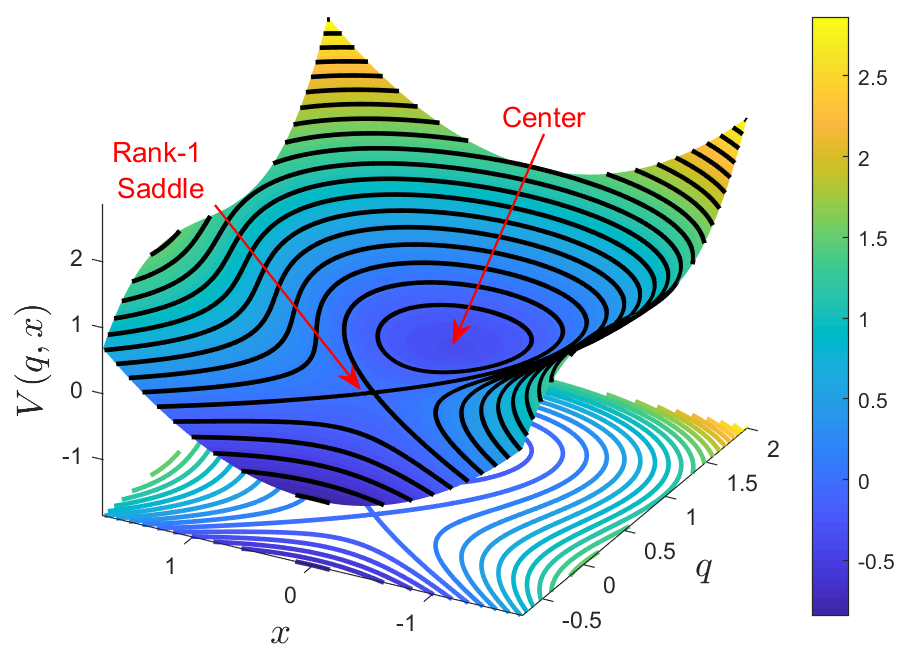
\includegraphics[scale=0.25]{fig6a.png}
		B)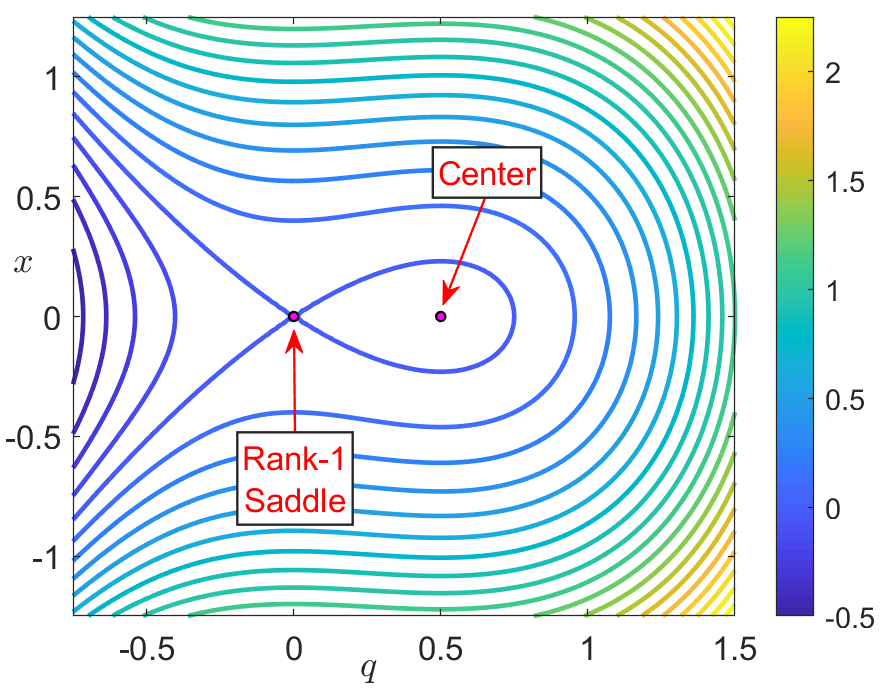
\includegraphics[scale=0.23]{fig6b.png}
		C)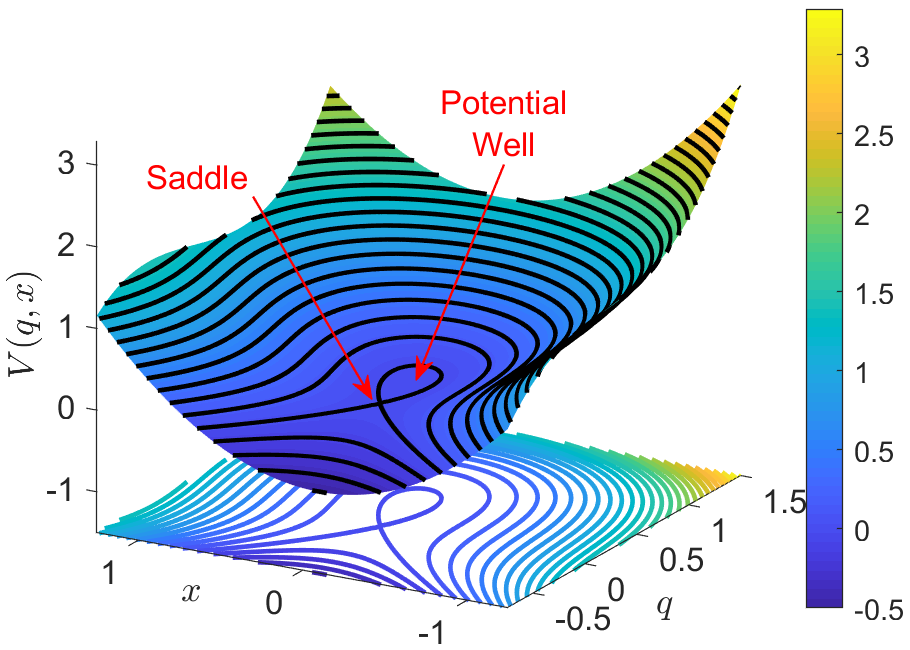
\includegraphics[scale=0.25]{fig6c.png}
		D)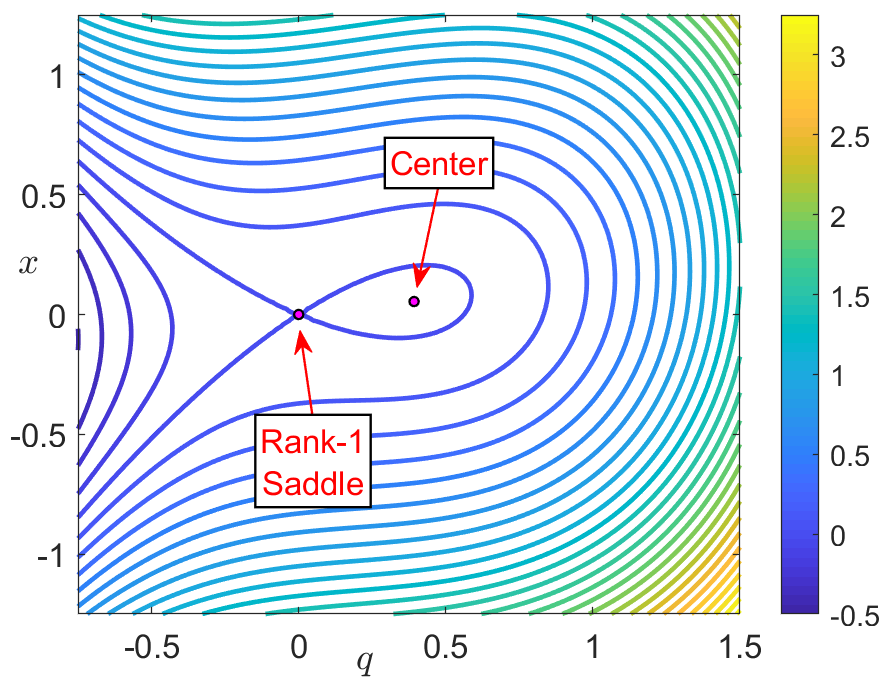
\includegraphics[scale=0.23]{fig6d.png}
		E)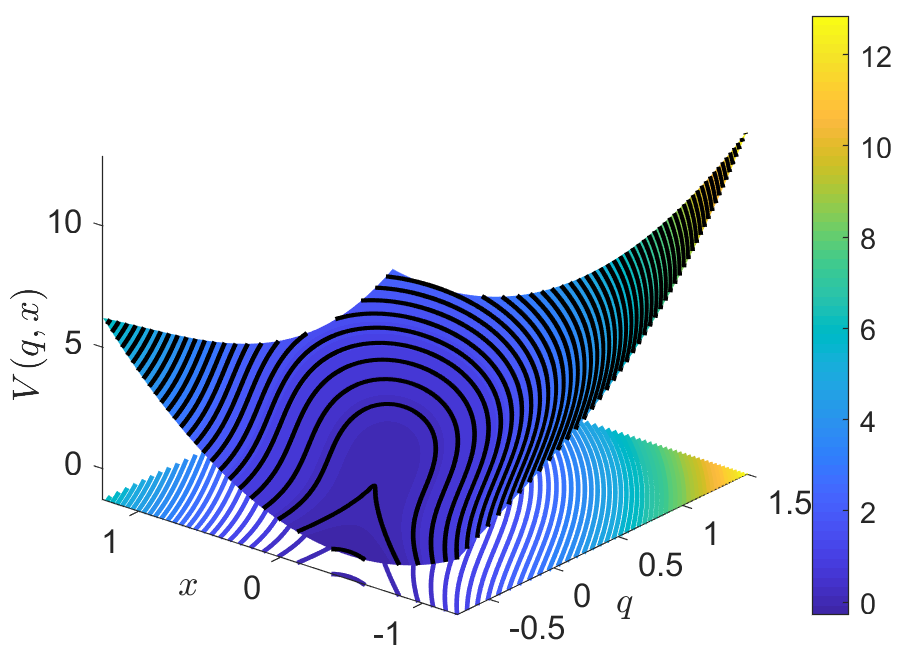
\includegraphics[scale=0.25]{fig6e.png}
		F)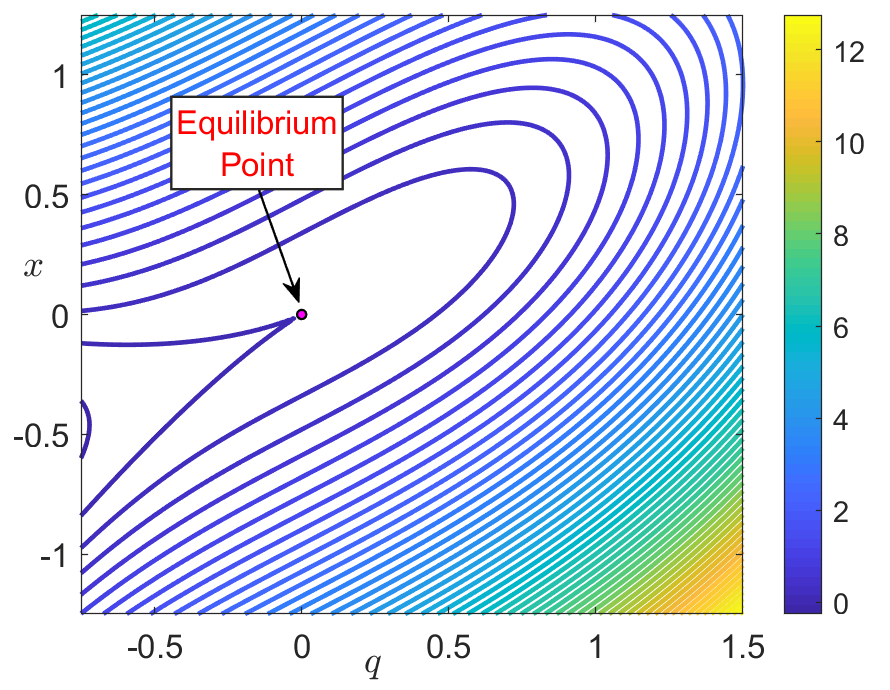
\includegraphics[scale=0.23]{fig6f.png}
	\end{center}
	
	\caption{Geometry of the PES (left-column) and equipotentials in configuration space  (right column) for the model parameters $\mu = 0.25$, $\alpha = 2$ and $\omega = 1.25$. A) and B) correspond to $\varepsilon = 0$; C) and D) represent the case $\varepsilon = 0.25$; E) and F) are for the critical coupling strength $\varepsilon = 25/9$.}
	\label{fig:figpes_2dof}
\end{figure} 

At this point, we carry out a linear stability analysis to show that the equilibrium point at the origin is an index-1 saddle of the PES. This analysis will be useful for computing the unstable periodic orbit (UPO), or normally hyperbolic invariant manifold (NHIM), associated to the index-1 saddle. Also, it will allow us to determine the NHIM's invariant stable and unstable manifolds that act as codimension one impenetrable barriers on the constant energy hypersurface. The global geometry of these invariant manifolds is paramount for quantifying the reaction rate across the phase space bottleneck in the neighborhood of the index-1 saddle. The Jacobian matrix for the Hamiltonian system in Eq. \eqref{eq:hameq_2dof} is given by:
\begin{equation}
J(q,x,p,p_x) = 
\begin{pmatrix}
0 & 0 & 1 & 0 \\[.1cm]
0 & 0 & 0 & 1 \\[.1cm]
2\sqrt{\mu} - 2\alpha q - \varepsilon & \varepsilon & 0 & 0 \\[.1cm]
\varepsilon & -\omega^2 - \varepsilon & 0 & 0
\end{pmatrix}
\end{equation}
The stability of $\mathbf{x}_1^e = (0,0,0,0) $ is given by the eigenvalues of the Jacobian:
\begin{equation}
J(\mathbf{x}_1^e) = 
\begin{pmatrix}
0 & 0 & 1 & 0 \\[.1cm]
0 & 0 & 0 & 1 \\[.1cm]
2\sqrt{\mu} - \varepsilon & \varepsilon & 0 & 0 \\[.1cm]
\varepsilon & -\omega^2 - \varepsilon & 0 & 0
\end{pmatrix}
\label{eq:jacobian_2dof}
\end{equation}
If the system is decoupled, i.e. $\varepsilon = 0$, the eigenvalues are given by $\pm \lambda_0$ and $\pm \omega_0 \, i$, where 
\begin{equation}
\lambda_0 = \sqrt[4]{4\mu} \;,\quad \omega_0 = \omega
\end{equation}
Therefore, the origin is an index-1 saddle equilibrium point, since the linearized system has exactly one pair of real eigenvalues $ \pm \lambda_0$ and the saddle plane is spanned by their eigenvectors. We know from the Moser's generalization of the Lyapunov Subcenter Theorem \cite{wiggins2013normally,wiggins2003applied} that when the energy of the system is above that of the index-1 saddle, there is a two dimensional plane spanned by the eigenvectors of $\pm \omega_0 \, i$, known as the center invariant manifold. This invariant manifold with normal hyperbolicity is known as a NHIM and in the context of Hamiltonian systems with 2 DoF is an UPO and has the topology of a circle $S^1$. As the energy of the system is increased above the energy of the index-1 saddle at the origin, a bottleneck structure opens in phase space connecting dynamically different regions and allowing trajectories to move between them. This phenomenon results in a phase space transport mechanism. This framework of understanding chemical reactions is realized by computing the stable and unstable manifolds associated with the unstable periodic orbit. These invariant manifolds have cylindrical geometry, that is $\mathbb{R} \times S^1$, and their global behavior is referred to as \textit{tube dynamics}. The cylindrical manifolds are codimension one on the constant three-dimensional energy hypersurface and therefore, act as impenetrable barriers separating reactive and non-reactive trajectories in the phase space. Thus, they determine the initial conditions that will pass through the bottleneck in some future time (or had passed through it in the past) during their evolution~\cite{wiggins_impenetrable_2001}. The UPO provides us with the scaffolding to construct the dividing surface that separates the trapped motion in the well region of the PES and the escape to infinity of particle trajectories through the phase space bottleneck.

\smallskip

We look now at the linear stability of the coupled system, that is $\varepsilon \neq 0$. In this case, the reaction and bath DoF are coupled and we expect  chaotic trajectories to appear, having a significant influence on the reaction rate. However, the geometry of the NHIM and its invariant manifolds still governs this reaction mechanism. A simple analysis reveals that the square of the eigenvalues of the Jacobian matrix at the origin are given by:
\begin{equation}
\xi =\dfrac{\lambda_0^2 - \omega_0^2}{2} - \varepsilon \pm \sqrt{\left(\dfrac{\lambda_0^2 + \omega_0^2}{2}\right)^2 + \varepsilon^2} \;\;.
\label{eq:eig_ham_2dof}
\end{equation}
as a function of the coupling strength $\varepsilon$ and the squares of the eigenvalues of the uncoupled system $\lambda_0^2$ and $\omega_0^2$. Notice that when the condition $\omega_0^2 \leq \lambda_0^2$ holds, the two possible values of $\xi$ have opposite signs for all $\varepsilon > 0$. Moreover, under the assumption $\omega_0^2 > \lambda_0^2$, the two values of $\xi$ have opposite sign whenever $0 < \varepsilon < \varepsilon_c$ is satisfied, where the critical coupling strength $\varepsilon_c$ is given by Eq. \eqref{eq:crit_epsi}. If we denote $\xi_{1,\varepsilon}$ and $\xi_{2,\varepsilon}$ as the positive and negative roots respectively in Eq. \eqref{eq:eig_ham_2dof}, then the eigenvalues of the Jacobian matrix are $\pm \lambda_\varepsilon$ and $\pm \omega_\varepsilon i$ where
\begin{equation}
\lambda_\varepsilon = \sqrt{\xi_{1,\varepsilon}} \quad,\quad \omega_\varepsilon = \sqrt{|\xi_{2,\varepsilon}|} \;.
\label{eq:eigenvalues_2dof}
\end{equation}
This argument shows that the equilibrium point at the origin is still an index-1 saddle for the coupled system under the conditions discussed above. In particular, when the coupling between the reaction and the bath DoF is weak, that is $\varepsilon \ll 1$, we have 
\begin{equation}
\lambda_\varepsilon \approx \sqrt{\lambda_0^2 - \varepsilon} \quad,\quad \omega_\varepsilon \approx \sqrt{\omega_0^2 + \varepsilon} \;,
\end{equation}
which confirms that the index-1 saddle structure of the equilibrium point at the origin persists under small perturbations. To finish the linear stability analysis of the equilibrium point at the origin, we compute the eigenvectors. Those associated with the real eigenvalues $\beta = \pm \lambda_{\varepsilon}$ correspond to the tangent directions of the unstable and stable manifolds, respectively, of the NHIM at the index-1 saddle, are given by:
\begin{equation}
\mathbf{u}_{\pm} = \left(1,\frac{\varepsilon}{\varepsilon + \left(\lambda^2_\varepsilon + \omega^2_0\right)},\pm\lambda_{\varepsilon},\pm\frac{\lambda_{\varepsilon} \, \varepsilon}{\varepsilon + \left(\lambda^2_\varepsilon + \omega^2_0\right)}\right) \;.
\label{eq:saddle_eigenv}
\end{equation}
The eigenvectors associated with the complex eigenvalues $\beta = \pm \omega_\varepsilon i$ span the center subspace of the NHIM at the index-1 saddle have the form:
\begin{equation}
\mathbf{w}_{\pm} = \left(\frac{\varepsilon}{\varepsilon - \left(\lambda^2_0 + \omega^2_\varepsilon\right)},1,\pm\frac{\omega_{\varepsilon} \, \varepsilon}{\varepsilon - \left(\lambda^2_0 + \omega^2_\varepsilon\right)}\, i,\pm\omega_{\varepsilon}\, i\right) \;.
\label{eq:center_eigenv}
\end{equation}
Therefore, we can write the solution to the linearized system at the index-1 saddle as:
\begin{equation}
\mathbf{x}(t) = C_1 e^{\lambda_\varepsilon t} \mathbf{u}_{+} + C_2 e^{-\lambda_\varepsilon t} \mathbf{u}_{-} + 2 Re\left(\eta e^{i\omega_\varepsilon t} \mathbf{w}_{+}\right)
\label{eq:geneq_lin_ham}
\end{equation}
where $C_1,C_2 \in \mathbb{R}$ and $\eta = \eta_1 + \eta_2 \, i \in \mathbb{C}$ are constants to be determined from an initial condition. This general solution to the linear system can be used in order to select an initial guess to search for the NHIM and construct its stable and unstable manifolds by using the differential correction and numerical continuation method \cite{Koon2011,naik2017geometry,naik2019b,GG2019}. 

\smallskip

Once we have established the framework to discuss Hamiltonian saddle-node bifurcations in two DoF systems, we move on to study the changes in the geometry of the relevant phase space invariant manifolds that govern reaction dynamics in terms of the coupling strength. We do so by applyng the method of Lagrangian descriptors (LDs), see e.g. \cite{mancho2013lagrangian,lopesino2017}, and in particular we use its variable integration time version \cite{junginger2017chemical,naik2019b,GG2019} since trajectories can escape to infinity in finite time for the dynamical system we are considering. We also take advantage of the differential correction method to compute UPOs and numerical continuation and globalization for the construction of their invariant stable and unstable manifolds. For a detailed description of these nonlinear techniques, the interested reader can refer to \cite{Koon2011,naik2017geometry,naik2019b,GG2019}.

\smallskip

We start by fixing a total energy $H_0$ of the system. Since the model has two DoF, we know that dynamics takes place on a three-dimensional energy hypersurface embedded in the four-dimensinal phase space. This energy hypersurface is described by the set:
\begin{equation}
\begin{split}
\mathcal{S}(H_0) &= \left\lbrace (q,x,p,p_x) \in \mathbb{R}^4 \; \big|\; \dfrac{1}{2} \left(p^2 + p_x^2 \right) - \sqrt{\mu} \, q^2 + \frac{\alpha}{3} \,q^3 + \dfrac{\omega^2}{2} x^2 + \dfrac{\varepsilon}{2} \left(x-q\right)^2 = H_0 \right\rbrace
\end{split}
\end{equation}
The projection of the energy surface onto configuration space is:
\begin{equation}
\begin{split}
\mathcal{C}(H_0) &= \left\lbrace (q,x) \in \mathbb{R}^2 \; \big|\; V(q,x) \leqslant H_0 \right\rbrace \\ 
&= \left\lbrace (q,x) \in \mathbb{R}^2 \; \big|\; - \sqrt{\mu} \, q^2 + \frac{\alpha}{3} \,q^3 + \dfrac{\omega^2}{2} x^2 + \dfrac{\varepsilon}{2} \left(x-q\right)^2 \leqslant H_0 \right\rbrace
\end{split} \;,
\label{eq:hillsreg}
\end{equation}
which denotes configurations with positive kinetic energy, and is known in Celestial Mechanics as the \textit{Hill's region}. The boundary of $\mathcal{C}(H_0)$ is defined as the locus of points in the $(q,x)$ plane where the kinetic energy is zero, that is $H_0 = V(q,x)$, and is called the \textit{zero velocity curve}. The configuration space coordinates of the trajectories can only evolve inside the Hill's region, shown as white regions in Fig. \ref{fig:EnergySurf_Hills}. In order to identify the invariant manifolds, we take two dimensional slices of the energy surface and determine the intersection of the invariant manifolds with these low-dimensional slices. In particular, we calculate LDs and compare with qualitative understandings from Poincar\'e surfaces of section (SOSs). The isoenergetic SOSs chosen are:
\begin{align}
\mathcal{U}_{qp}^{+} &= \left\lbrace (q,x,p,p_x) \in \mathbb{R}^4 \; \big| \; x = 0 \; ,\; p_x(q,x,p;H_0) \geq 0 \right\rbrace \label{eq:sos_qp} \\[.1cm]
\mathcal{U}_{xp_x}^{+} &= \left\lbrace (q,x,p,p_x) \in \mathbb{R}^4 \; \big| \; q = q_e \; , \; p(q,x,p_x;H_0) \geq 0 \right\rbrace 
\label{eq:sos_xpx}
\end{align}
where $q_e$ is the first configuration space coordinate of the center equilibrium $\mathbf{x}_2^e$ in Eq. \eqref{eq:cfSp_eqCoords}.

\begin{figure}[!ht]
	\begin{center}		
		A)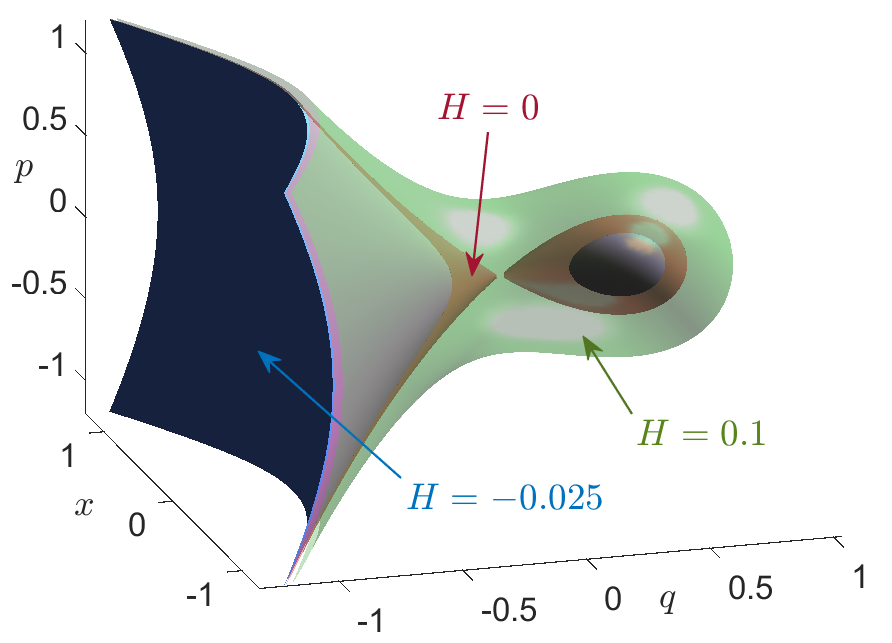
\includegraphics[scale=0.26]{fig7a}
		B)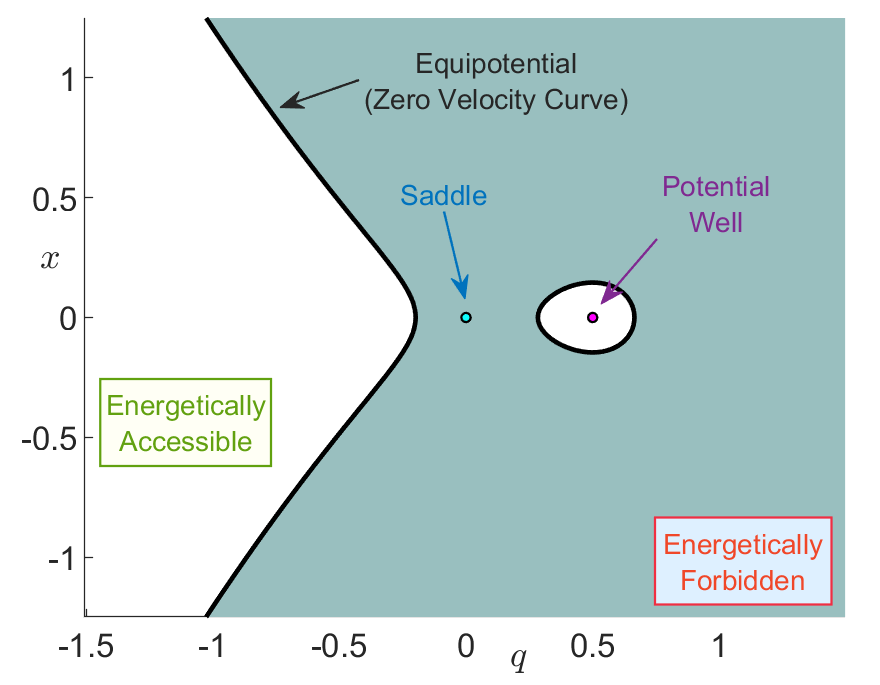
\includegraphics[scale=0.26]{fig7b}
		C)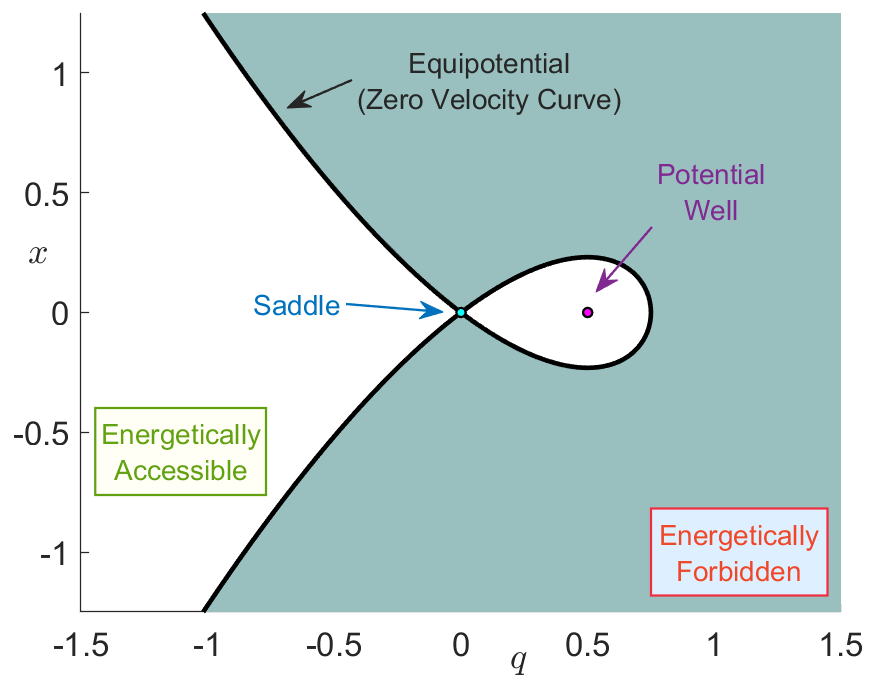
\includegraphics[scale=0.26]{fig7c}
		D)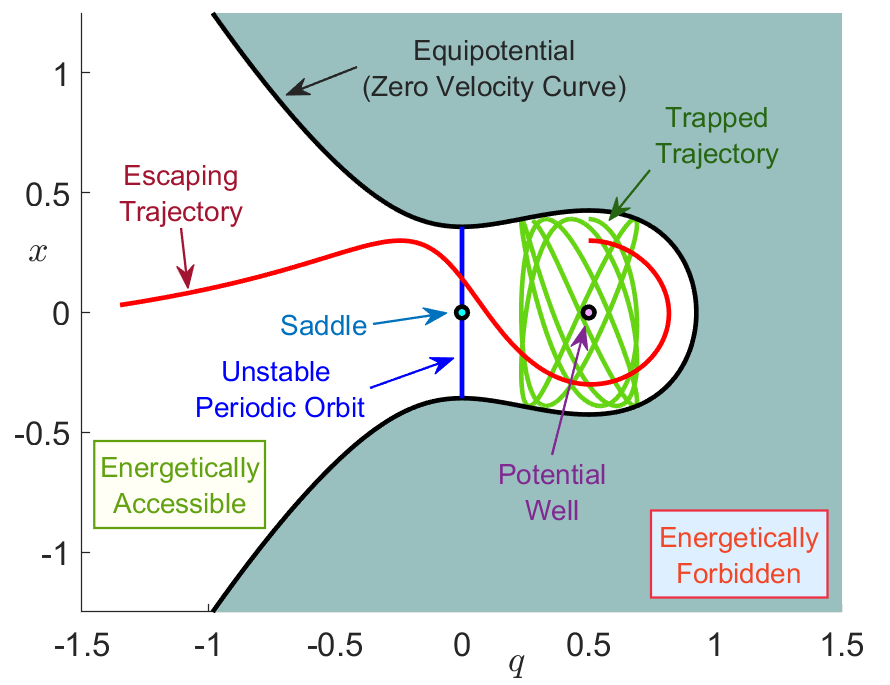
\includegraphics[scale=0.26]{fig7d}
	\end{center}
	
	\caption{A) Phase space energy surface inside which motion takes place for three different values of the energy; B) Configuration space projection for an energy $H = -0.025$ below the barrier energy; C) for the index-1 saddle energy $H = 0$; D) for the energy $H = 0.1$, above the barrier energy. The parameter values chosen are $\mu = 0.25$, $\alpha = 2$, $\omega = 1.25$ and $\varepsilon = 0$. We have marked the energy accessible regions in white and the forbidden regions in dark grey. The equipotential in black marks the zero velocity curve for which the kinetic energy of the system is zero.}
	\label{fig:EnergySurf_Hills}
\end{figure}

We focus first on describing the dynamics for the uncoupled system ($\varepsilon = 0$). In this case the ``reaction'' and ``bath'' DoF are uncoupled, and therefore, the system is integrable and the trajectories are regular. The total energy can be partitioned among each DoF separately:
\begin{equation}
H(q,x,p,p_x) = \underbrace{\frac{1}{2} p^2 - \sqrt{\mu} \, q^2 + \frac{\alpha}{3} q^3}_{H_r(q,p)} + \underbrace{\frac{1}{2} \, p_x^2 + \frac{\omega^2}{2} x^2}_{H_b(x,p_x)} \;,
\end{equation}
where $H_r$ and $H_b$ are the Hamiltonians for the reaction and bath DoF respectively. Given a fixed total energy of the system $H_0$, the \textit{necessary condition} in order for reaction to take place is that the total energy is above that of the barrier of the PES located at the origin, which is zero. For $H_0 \leq 0$ the energy surface divides phase space into two disconnected regions as illustrated in Fig. \ref{fig:EnergySurf_Hills}, so that we have bounded motion in the potential well region. In Fig. \ref{fig:LD_PS_uncoupled}, we compare the bounded trajectories (regular dynamics) of the system for $H_0 = 0$ by computing LDs and Poincar\'e section on the SOS $\mathcal{U}_{qp}^{+}$ in Eq. \eqref{eq:sos_qp}. Both methods clearly recover, the trajectories on tori, as known for integrable Hamiltonian systems \cite{Meyer2009}, that foliate the energy surface. We observe that the high values (white regions in Fig. \ref{fig:LD_PS_uncoupled} in the LD contour map recover the quasiperiodic trajectories, which is a consequence of the relationship between the convergence of time averages of LDs with the Ergodic Partition Theorem as explained in \cite{lopesino2017}. 

\begin{figure}[!ht]
	\begin{center}
		A)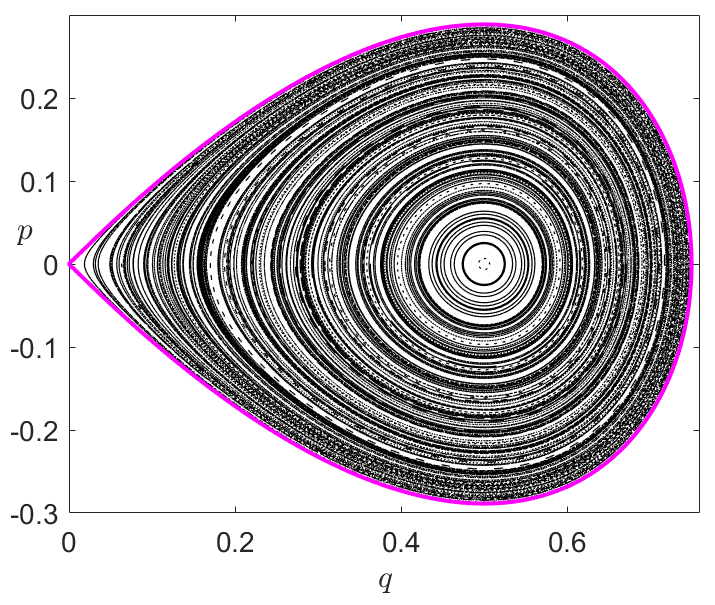
\includegraphics[scale=0.32]{fig8a}
		B)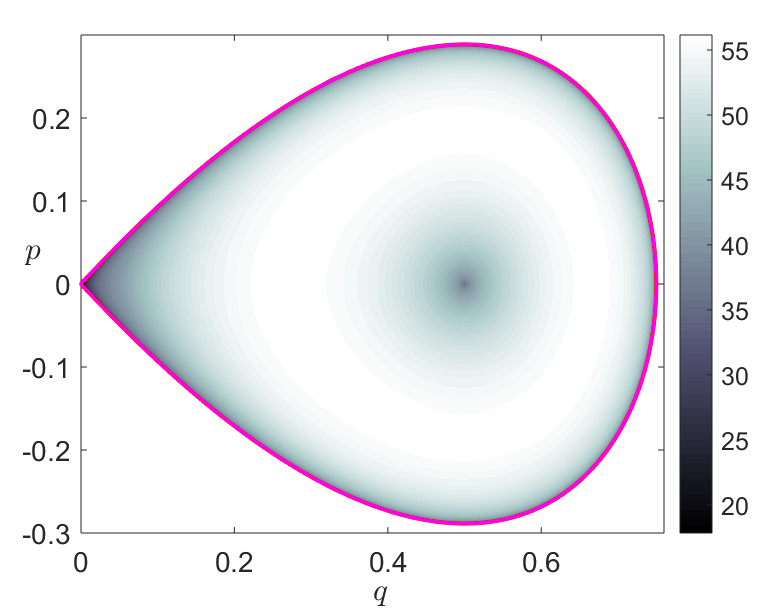
\includegraphics[scale=0.33]{fig8b}
	\end{center}
	
	\caption{Quasiperiodic trajectories describing regular motion in the potential well region of the PES for the uncoupled ($\varepsilon = 0$) Hamiltonian system with energy $H_0 = 0$. The model parameters chosen for this calculation are $\mu = 0.25$, $\alpha = 2$ and $\omega = 1.25$; A) Poincar\'e map; B) LDs obtained for an integration time $\tau = 20$. The curve in magenta depicts the energy boundary.}
	\label{fig:LD_PS_uncoupled}
\end{figure}

When the energy of the system is above the barrier, that is $H_0 > 0$, the topology of the energy surface changes and a phase space bottleneck opens up in the barrier region allowing the escape from the well as shown in Fig.~\ref{fig:EnergySurf_Hills} D). Thus, reaction can take place when trajectories cross the bottleneck, and we can define reaction when the $q$ configuration coordinae changes sign, passing from $q > 0$ to $q < 0$ or vice-versa.	Therefore, $q=0$ is a natural choice for defining in phase space a dividing surface (DS) separating reactants (bounded motion in the potential well region) from products (escape to infinity). Hence, the isoenergetic DS is given by:
\begin{equation}
\mathcal{D}(H_0) = \left\{ (q,x,p,p_x) \in \mathbb{R}^4 \; | \; q = 0 \;,\; 2H_0 = p^2 + p_x^2 + \omega^2 x^2 \right\} \;,
\end{equation}
which has the geometry of a 2-sphere, that is $S^2$ in the three-dimensional energy hypersurface. To be precise, it is an ellipsoid with semi-major axis $\sqrt{2H_0}$ in the $p$, $p_x$ axis, and $\sqrt{2H_0}/\omega$ in the $x$ axis. This ellipsoid has two hemispheres, known as the forward and backward DS with the form:
\begin{equation}
\begin{split}
\mathcal{D}_f(H_0) &= \left\{ (q,x,p,p_x) \in \mathbb{R}^4 \; | \; q = 0 \;,\; p =- \sqrt{2H_0 -  p_x^2 - \omega^2 x^2} \right\} \\[.1cm]
\mathcal{D}_b(H_0) &= \left\{ (q,x,p,p_x) \in \mathbb{R}^4 \; | \; q = 0 \;,\; p = +\sqrt{2H_0 -  p_x^2 - \omega^2 x^2} \right\} 
\end{split}
\;.
\end{equation}
Forward reaction occurs when trajectories cross $\mathcal{D}_f$ and escape from the potential well, and backward reaction when trajectories cross $\mathcal{D}_b$ and enter the well region. The forward and backward DS meet at the equator along the NHIM given by:
\begin{equation}
\mathcal{N}(H_0) = \left\{ (q,x,p,p_x) \in \mathbb{R}^4 \; | \; q = p = 0 \;,\; 2H_0 = p_x^2 + \omega^2 x^2 \right\} \;,
\end{equation}
which has the topology of $S^1$. To be precise, it is an ellipse with semiaxis $\sqrt{2H_0}$ in the $p_x$ direction and $\sqrt{2H_0}/\omega$ in the $x$ direction. As discussed earlier, for a 2 DoF Hamiltonian the NHIM is an unstable periodic orbit which extends the influence of the index-1 saddle equilibrium point of the PES, a configuration space concept, into phase space. We note that for $H_0 > 0$ the NHIM is the correct phase space structure that anchors the barriers to the reaction and carries the effect of the index-1 saddle equilibrium point to a range of energies as given by Moser's generalization of Lyapunov Subcenter Manifold Theorem \cite{wiggins2003applied}. The stable and unstable manifolds of the UPO are: 
\begin{equation}
\mathcal{W}^s = \Gamma \cup \mathcal{W}^s_l \quad , \quad \mathcal{W}^u = \Gamma \cup \mathcal{W}^u_l \;,
\end{equation}
where $\Gamma$ is the homoclinic orbit:
\begin{equation}
\Gamma = \left\{  (q,x,p,p_x) \in \mathbb{R}^4 \; | \; q > 0 \;,\; H_r(q,p) = 0 \;,\; H_b(x,p_x) = H_0 \right\} \;,
\end{equation}
and the left branches are:
\begin{equation}
\begin{split}
\mathcal{W}^s_l &= \left\{ (q,x,p,p_x) \in \mathbb{R}^4 \; | \; q < 0 \:,\; p > 0 \;,\; H_r(q,p) = 0 \;,\; H_b(x,p_x) = H_0 \right\} \\[.2cm]
\mathcal{W}^u_l &= \left\{ (q,x,p,p_x) \in \mathbb{R}^4 \; | \; q < 0 \:,\; p < 0 \;,\; H_r(q,p) = 0 \;,\; H_b(x,p_x) = H_0 \right\}
\end{split}
\;.
\end{equation}
Notice that the stable and unstable manifolds have the structure of a cartesian product of a curve in the $(q,p)$ saddle space and an ellipse in the $(x,p_x)$ center space, and thus become cylindrical (or \textit{tube}) manifolds. We show the energy surface for the uncoupled case ($\varepsilon = 0$) in Fig. \ref{fig:EnergySurf_Hills} A) for three energy values, where the bottleneck only opens for $H_0 > 0$. The NHIM computed using differential correction and continuation, and its invariant manifolds computed using globalization are shown in Fig. \ref{fig:set2_manifolds_upo_energysurf}A) for $H_0 = 0.05$ and $\varepsilon = 0$. 

\begin{figure}[!ht]
	\begin{center}
		A)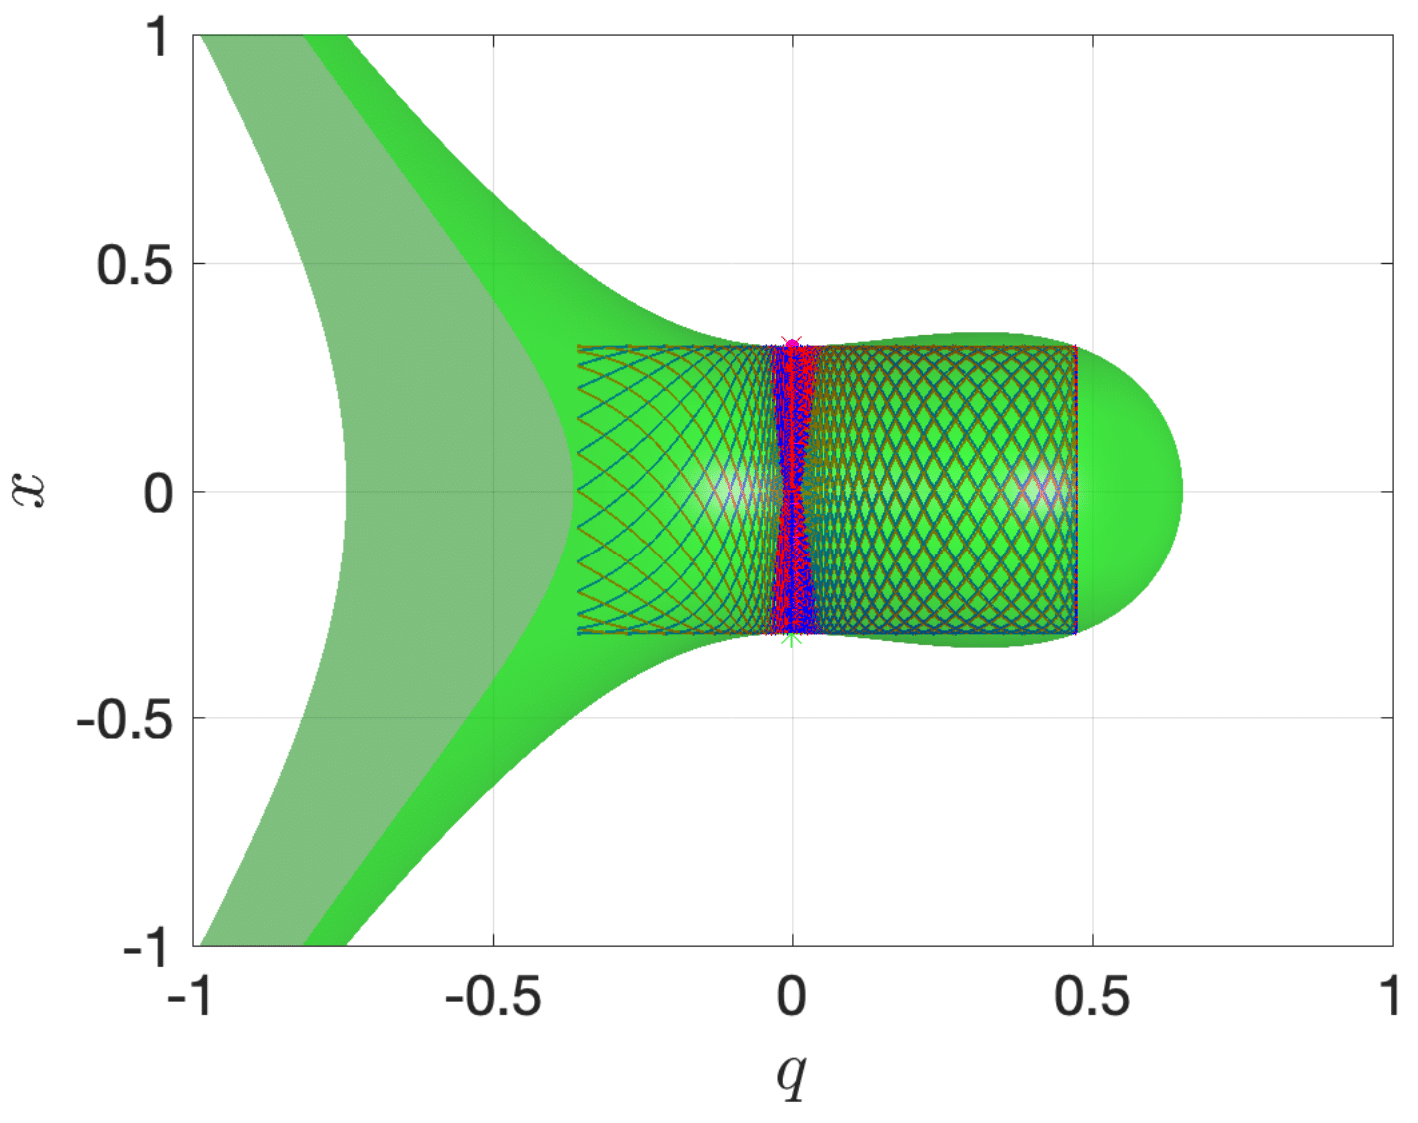
\includegraphics[width=0.35\linewidth]{fig9a.png}
		B)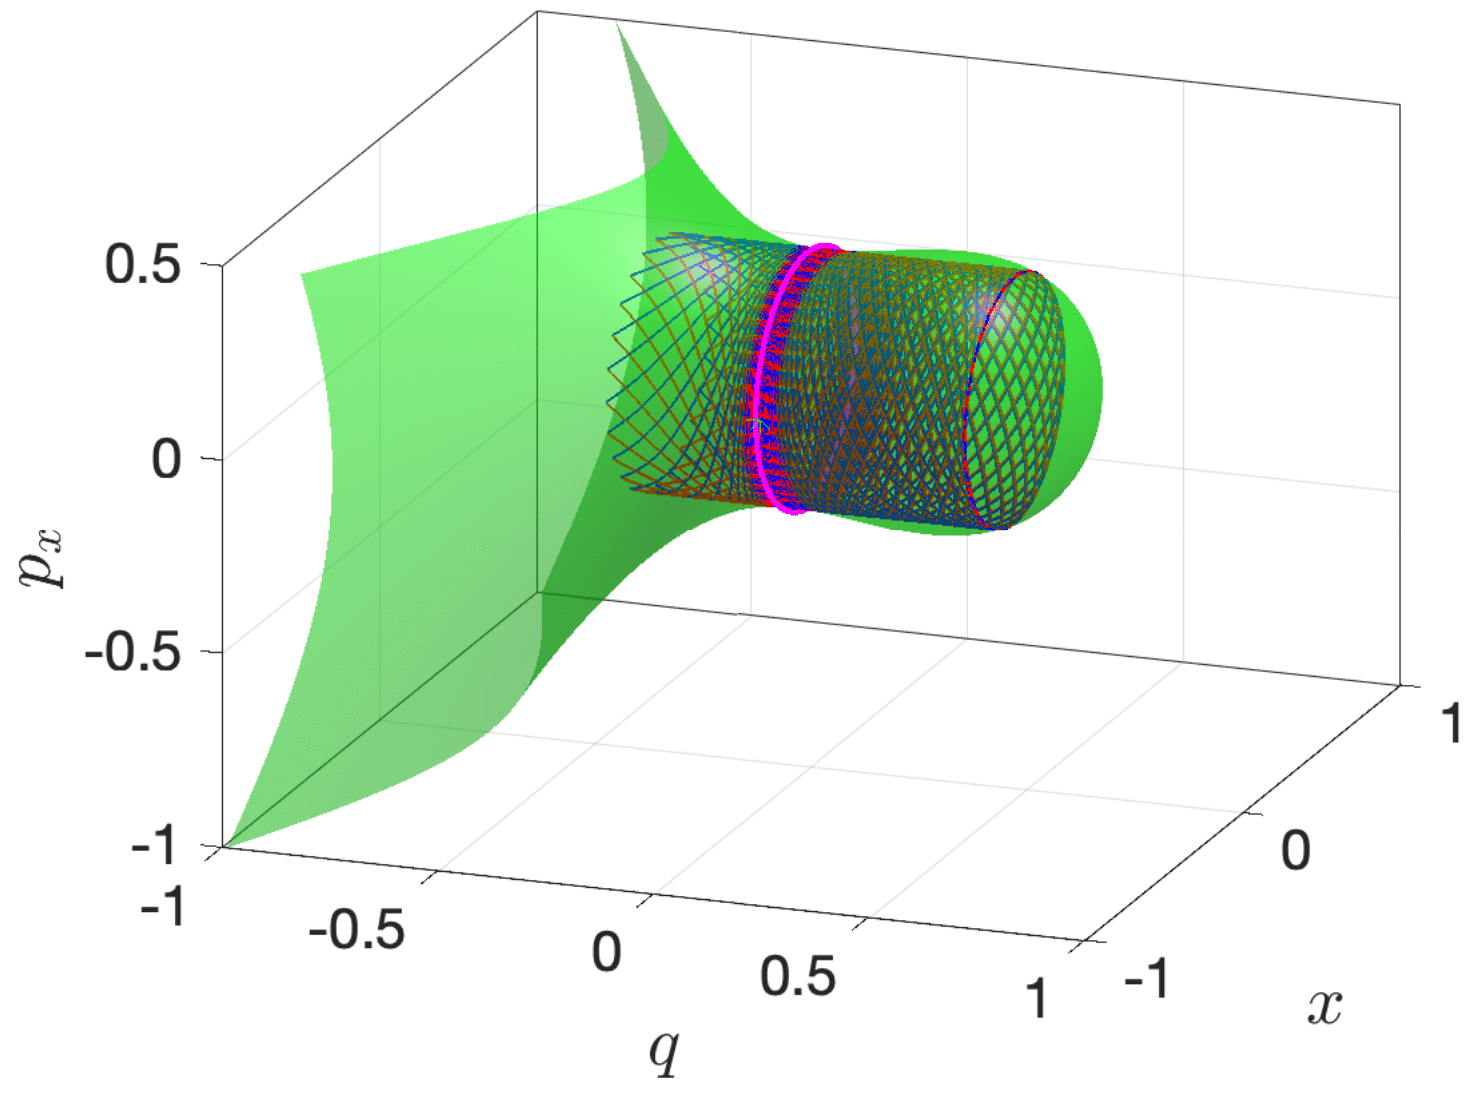
\includegraphics[width=0.4\linewidth]{fig9b.png}
		C)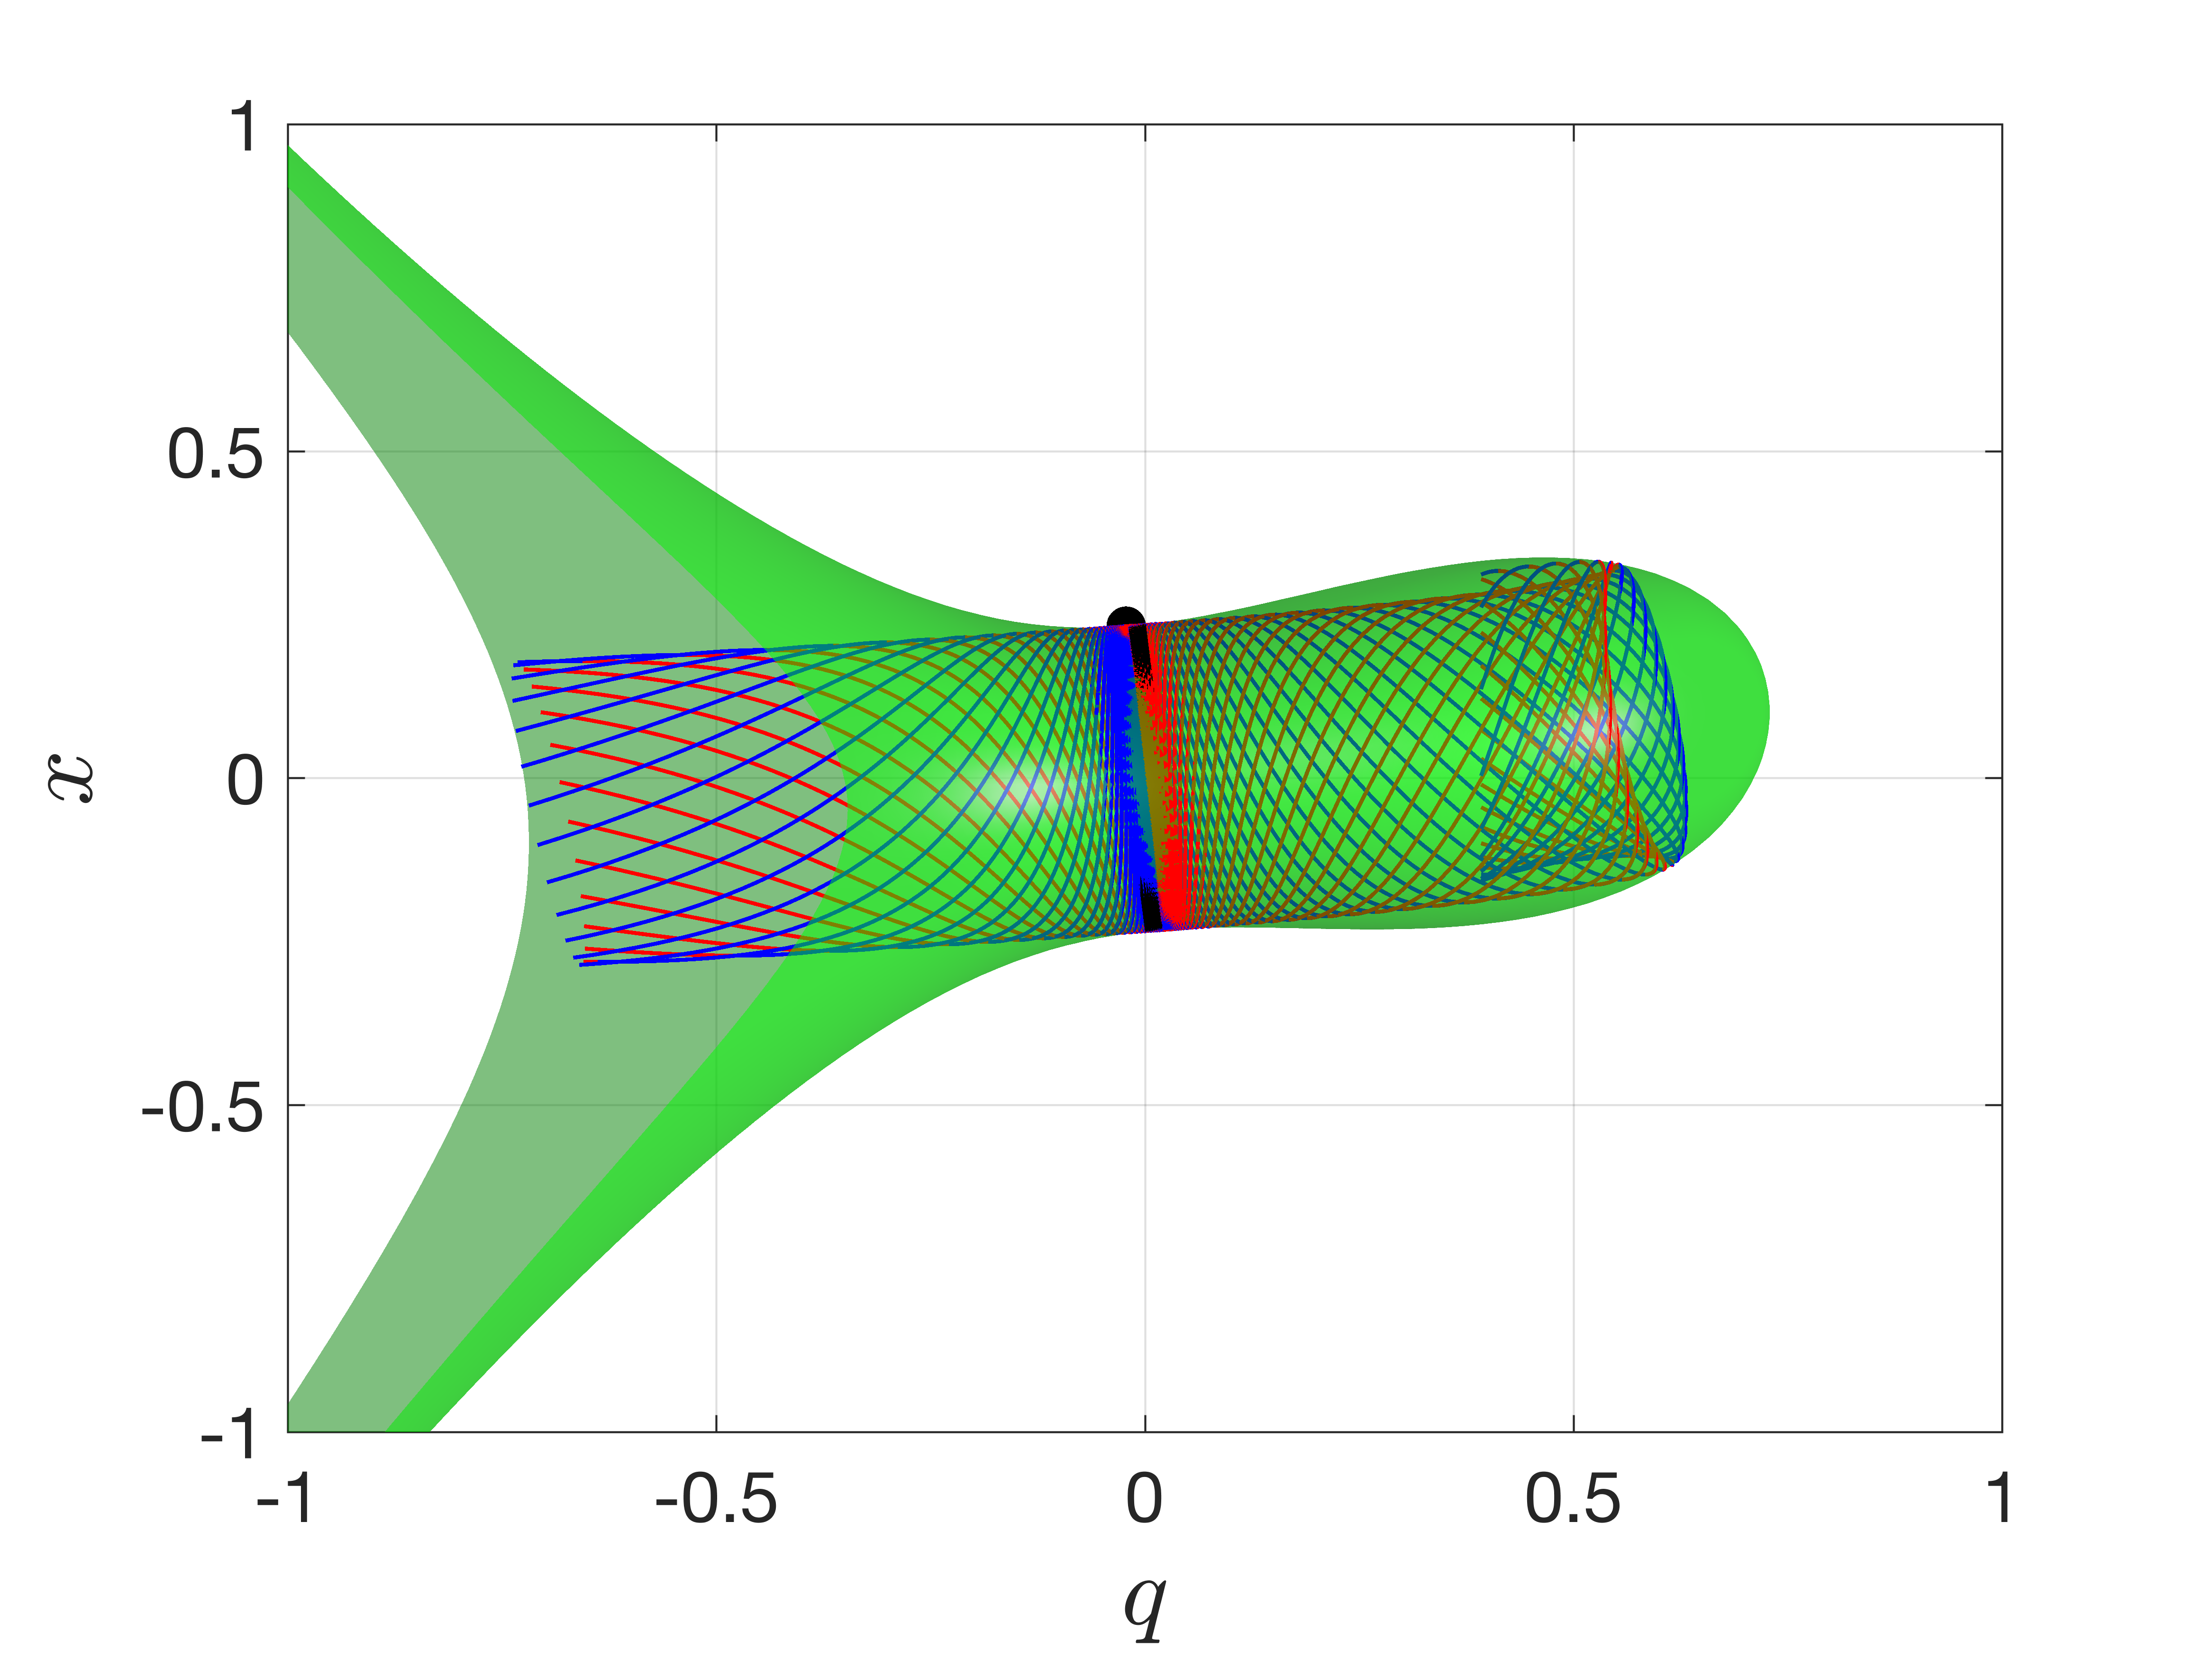
\includegraphics[width=0.39\linewidth]{fig9c.png}
		D)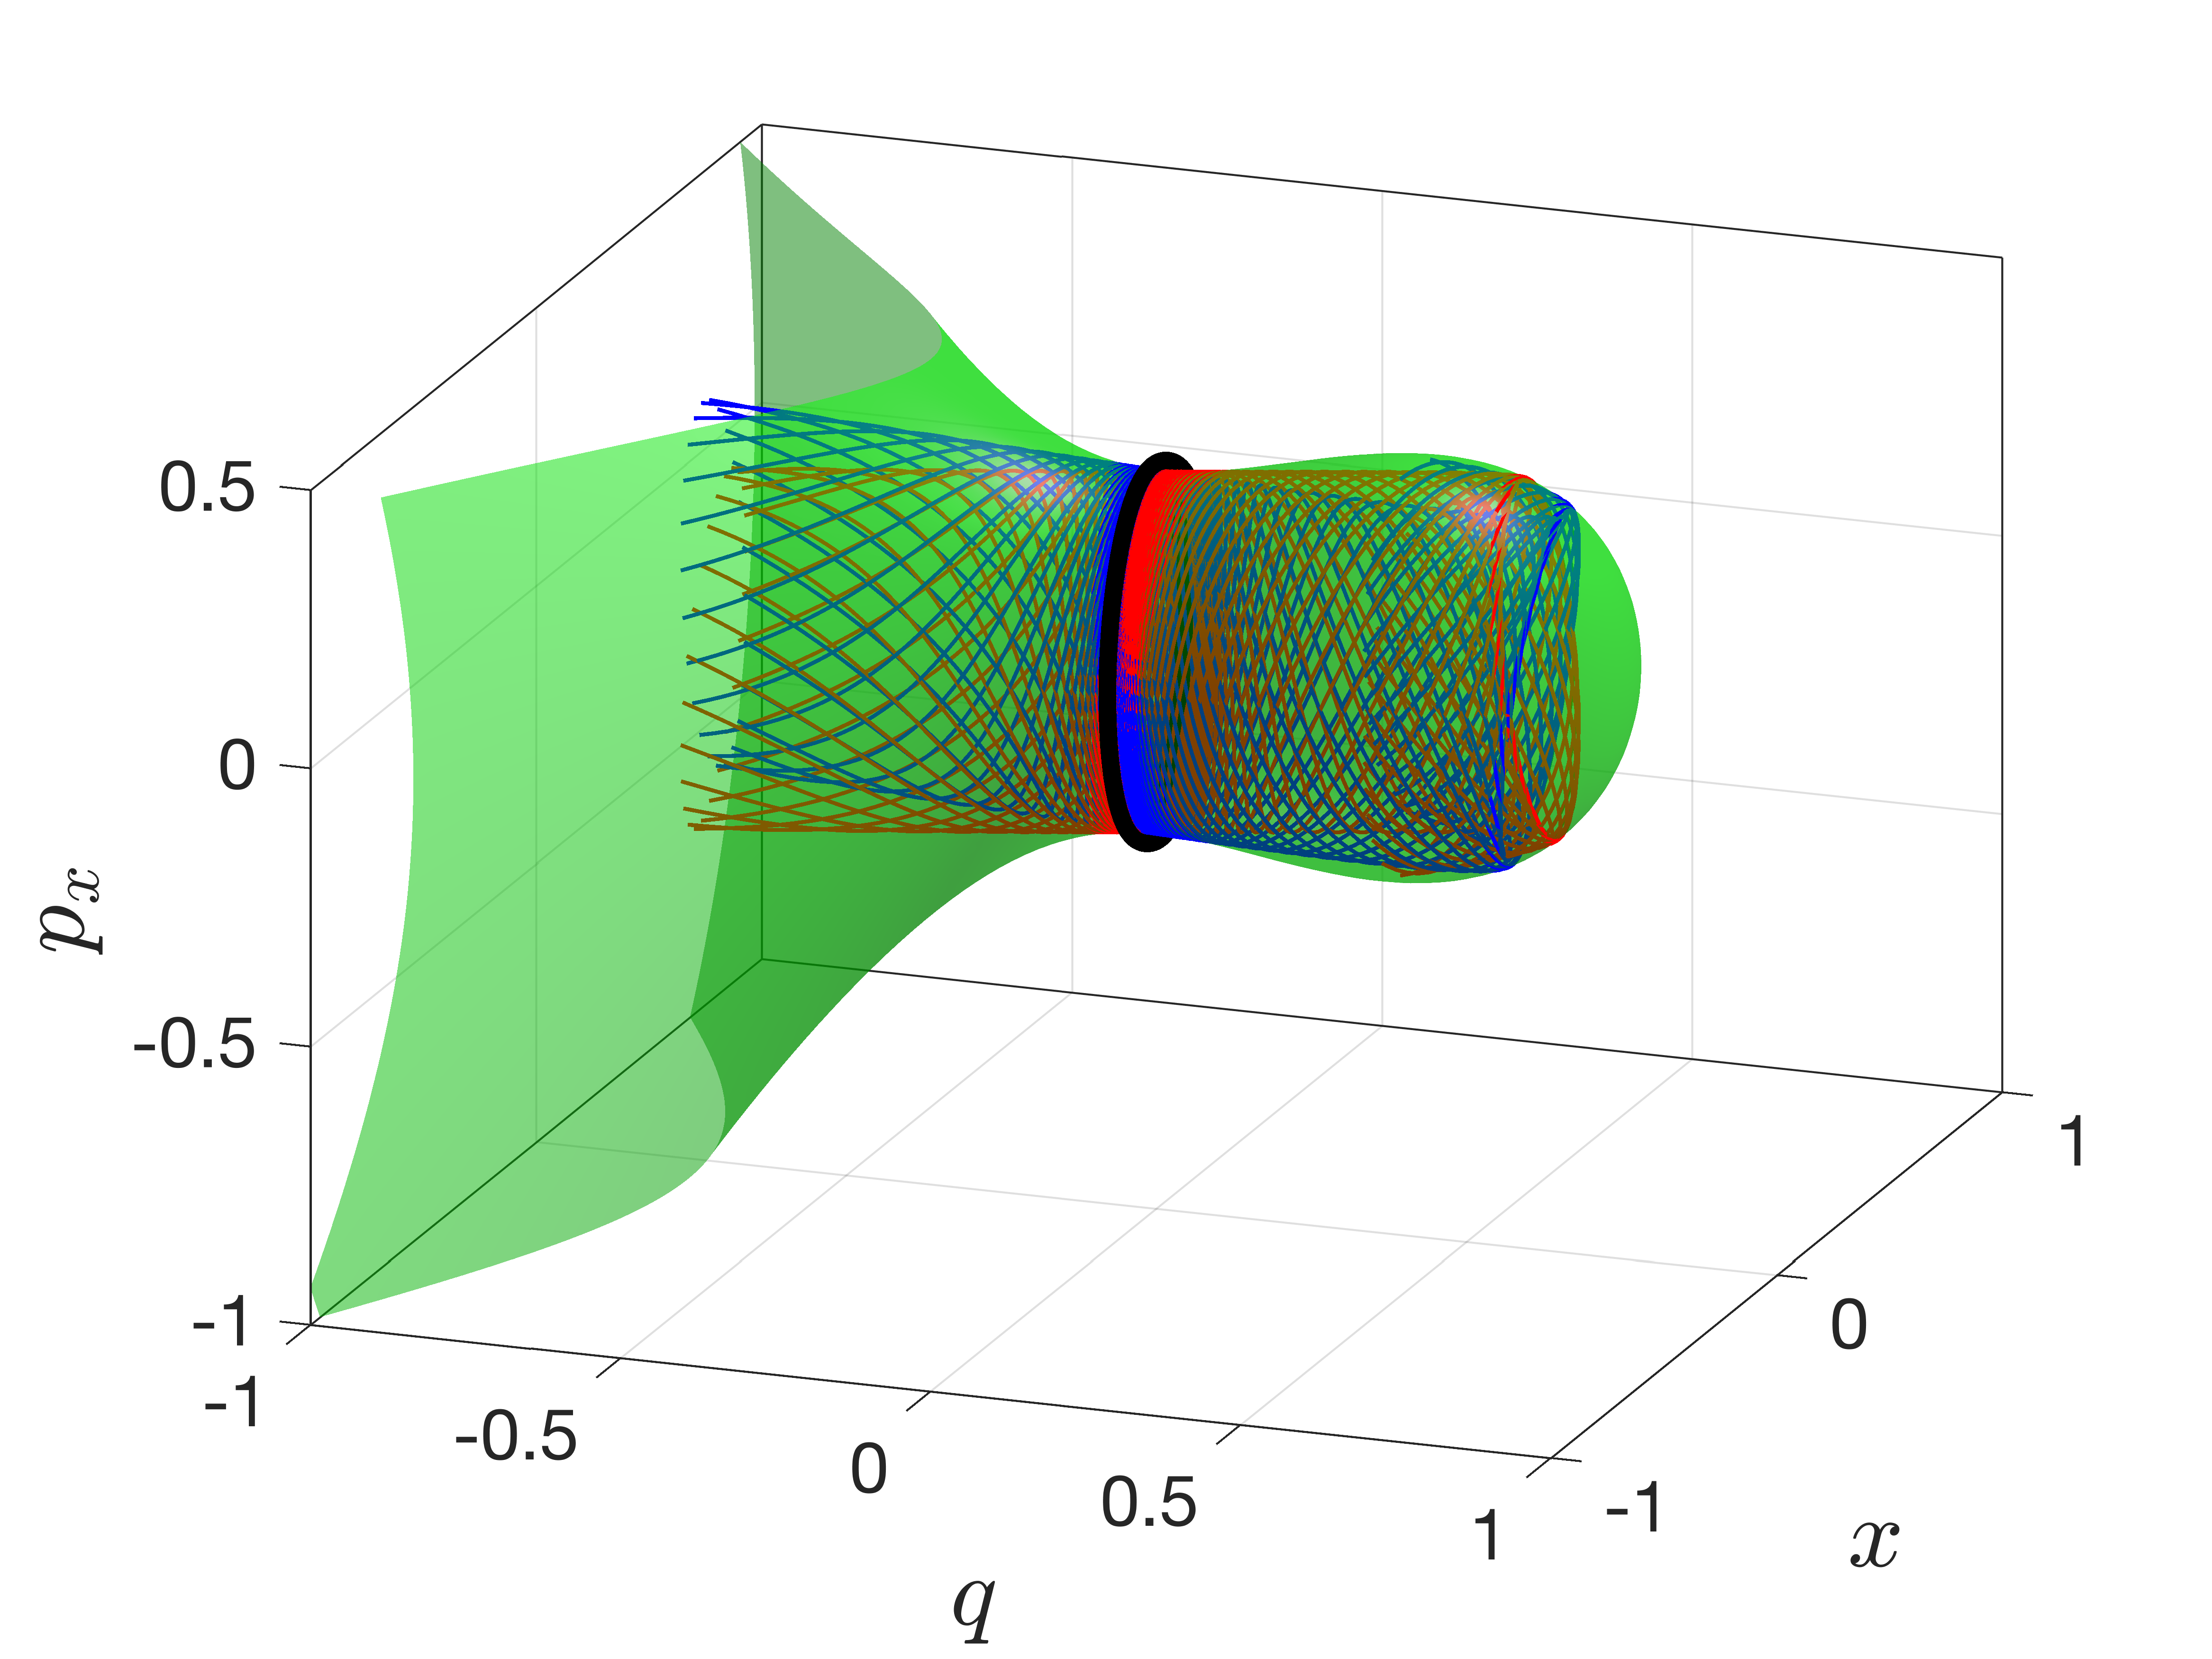
\includegraphics[width=0.4\linewidth]{fig9d.png}
	\end{center}
	
	\caption{Configuration and phase space view of the energy surface and the cylindrical manifolds of the UPO associated with the index-1 saddle in the bottleneck. Blue and red denote the stable and unstable manifolds respectively, and the green surface is the isosurface of total energy $H_0 = 0.05$. The magenta curve represents the UPO. A) and B) use $\epsilon = 0$; C) and D) $\epsilon = 0.25$.}
	\label{fig:set2_manifolds_upo_energysurf}
\end{figure}


We discuss next the dynamics of the system when the reactive and bath DoF are coupled, i.e. $\varepsilon \neq 0$, and we do so for $\varepsilon$ small. We can thus think about the resulting dynamics as a perturbation of the uncoupled case. Given an energy of the system below that of the barrier, that is $H_0 \leq 0$, the phase space bottleneck is closed and trajectories are trapped in the potential well region. However, due to the perturbation, the regular motion that existed on the tori in the uncoupled system is destroyed as given by the KAM theorem, and  therefore chaotic motion arises in some regions of the phase space. We illustrate the system's behavior for the energy $H_0 = 0$ (energy of the index-1 saddle) in Fig. \ref{fig:ps_vs_ld_1} using LDs and Poincar\'e maps on the SOSs described in Eqs. \eqref{eq:sos_qp} and \eqref{eq:sos_xpx}. We observe that there is a distinct correlation between the qualitative dynamics revealed by the Lagrangian descriptor (LD) contour maps and Poincar\'e sections. That is, chaotic regions of phase space which appear as a sea of points in the Poincar\'e section and hide the underlying structures of stable and unstable manifolds are completely resolved by LD contour maps where the tangled geometry of the manifolds is revealed by the points where the function is non-differentiable and attains a local minimum as has been shown in \cite{lopesino2017,naik2019b,GG2019}. The capability of LDs to identify the phase space structures relevant in chemical reaction dynamics can also be found in recent literature \cite{craven2016deconstructing,demian2017,Naik2019a,revuelta2019unveiling}. In addition, the generation of Poincar\'e sections relies on tracking the crossing of a 2D surface which can not be guaranteed in high dimensional phase space, while LDs just accumulate a positive scalar quantity along the trajectory and thus have potential to reveal high dimensional phase space structures.

\begin{figure}[!ht]
	\begin{center}		
		A)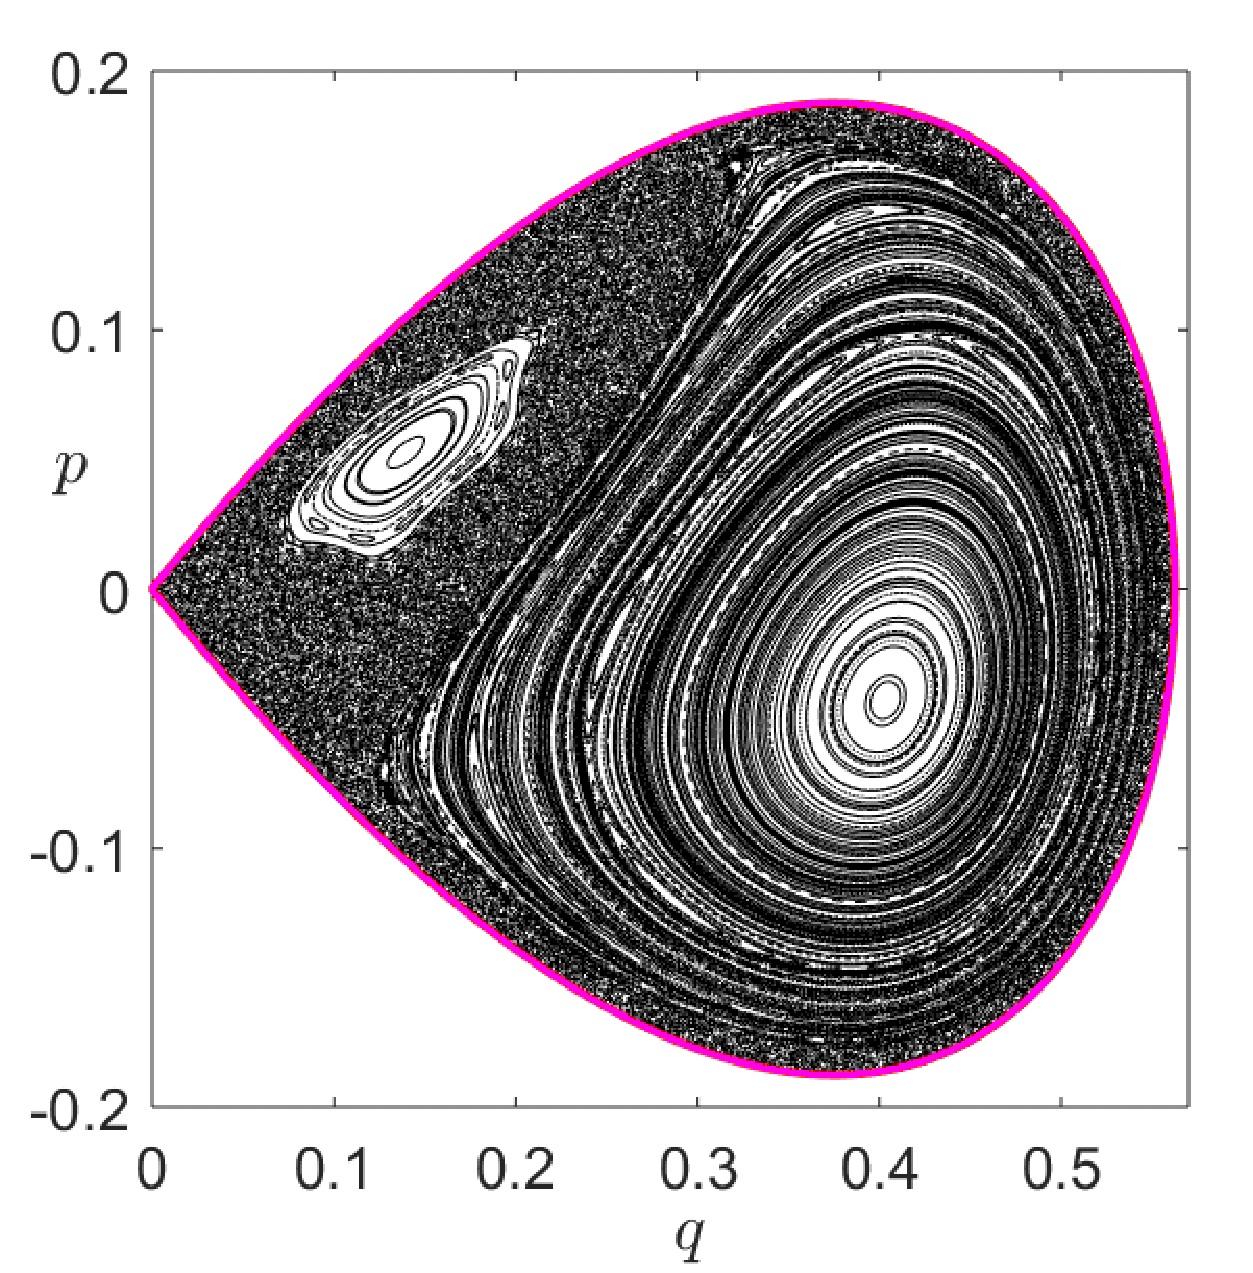
\includegraphics[scale=0.13]{fig10a.png}	
		B)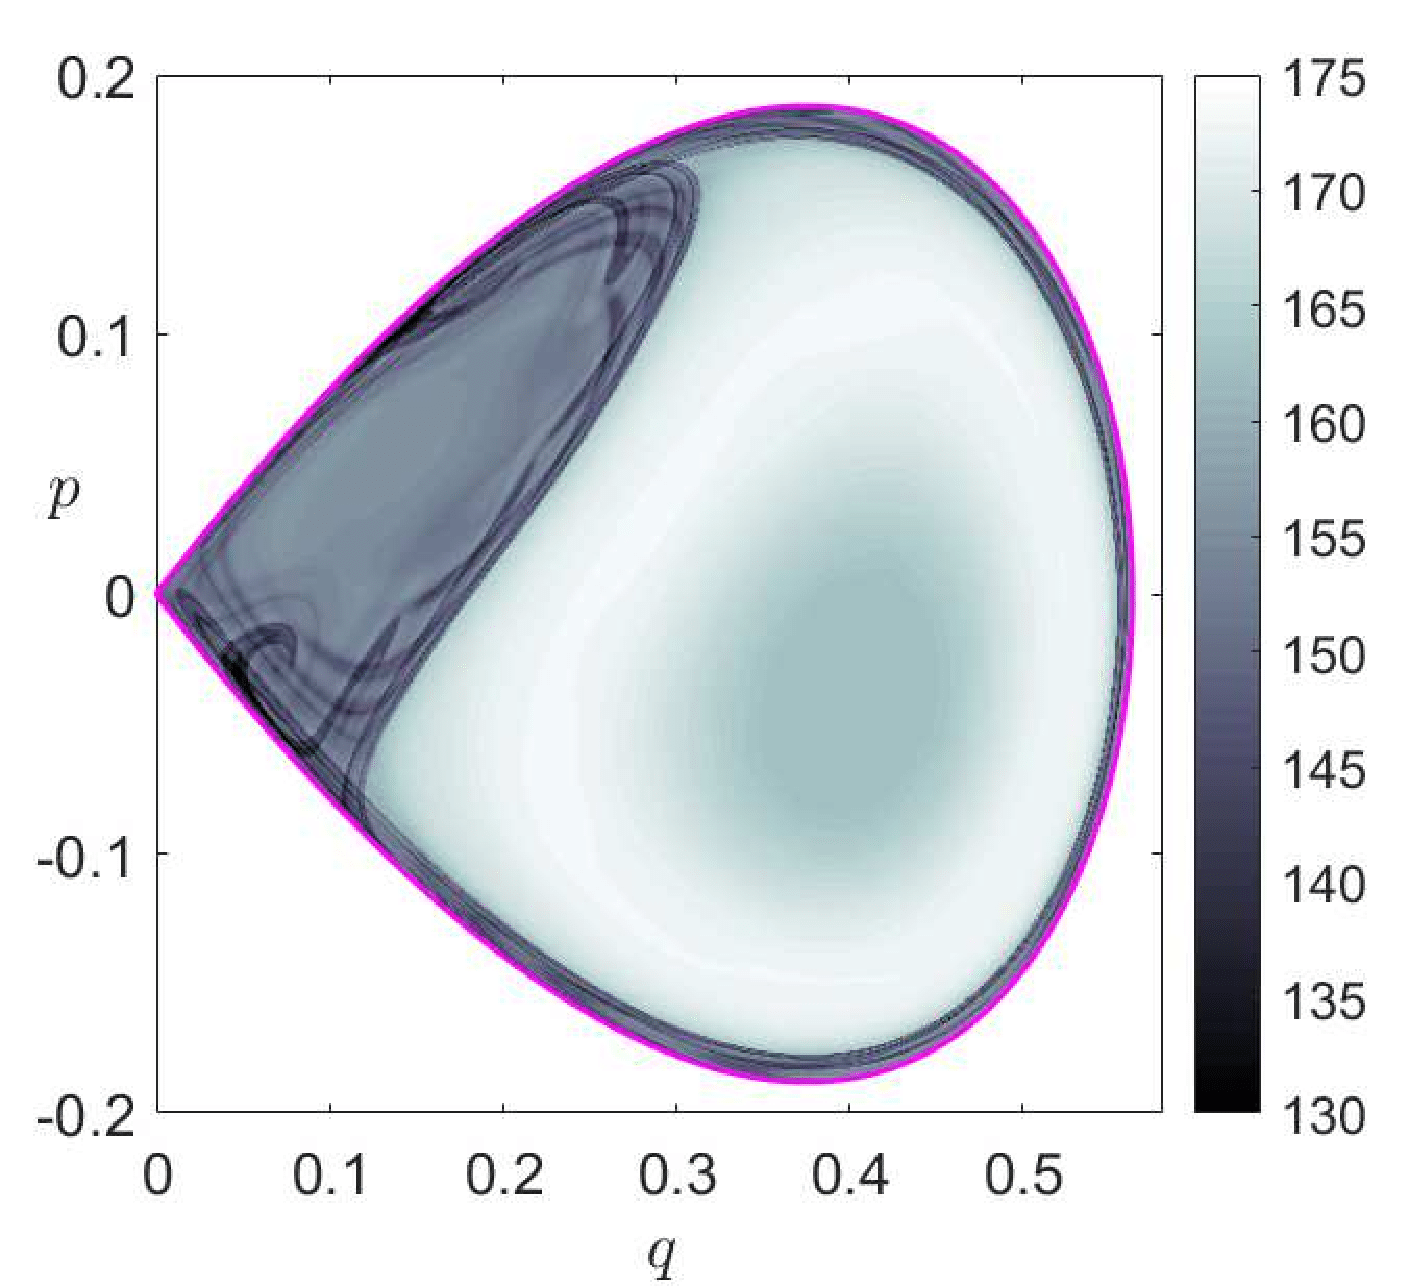
\includegraphics[scale=0.13]{fig10b.png}
		C)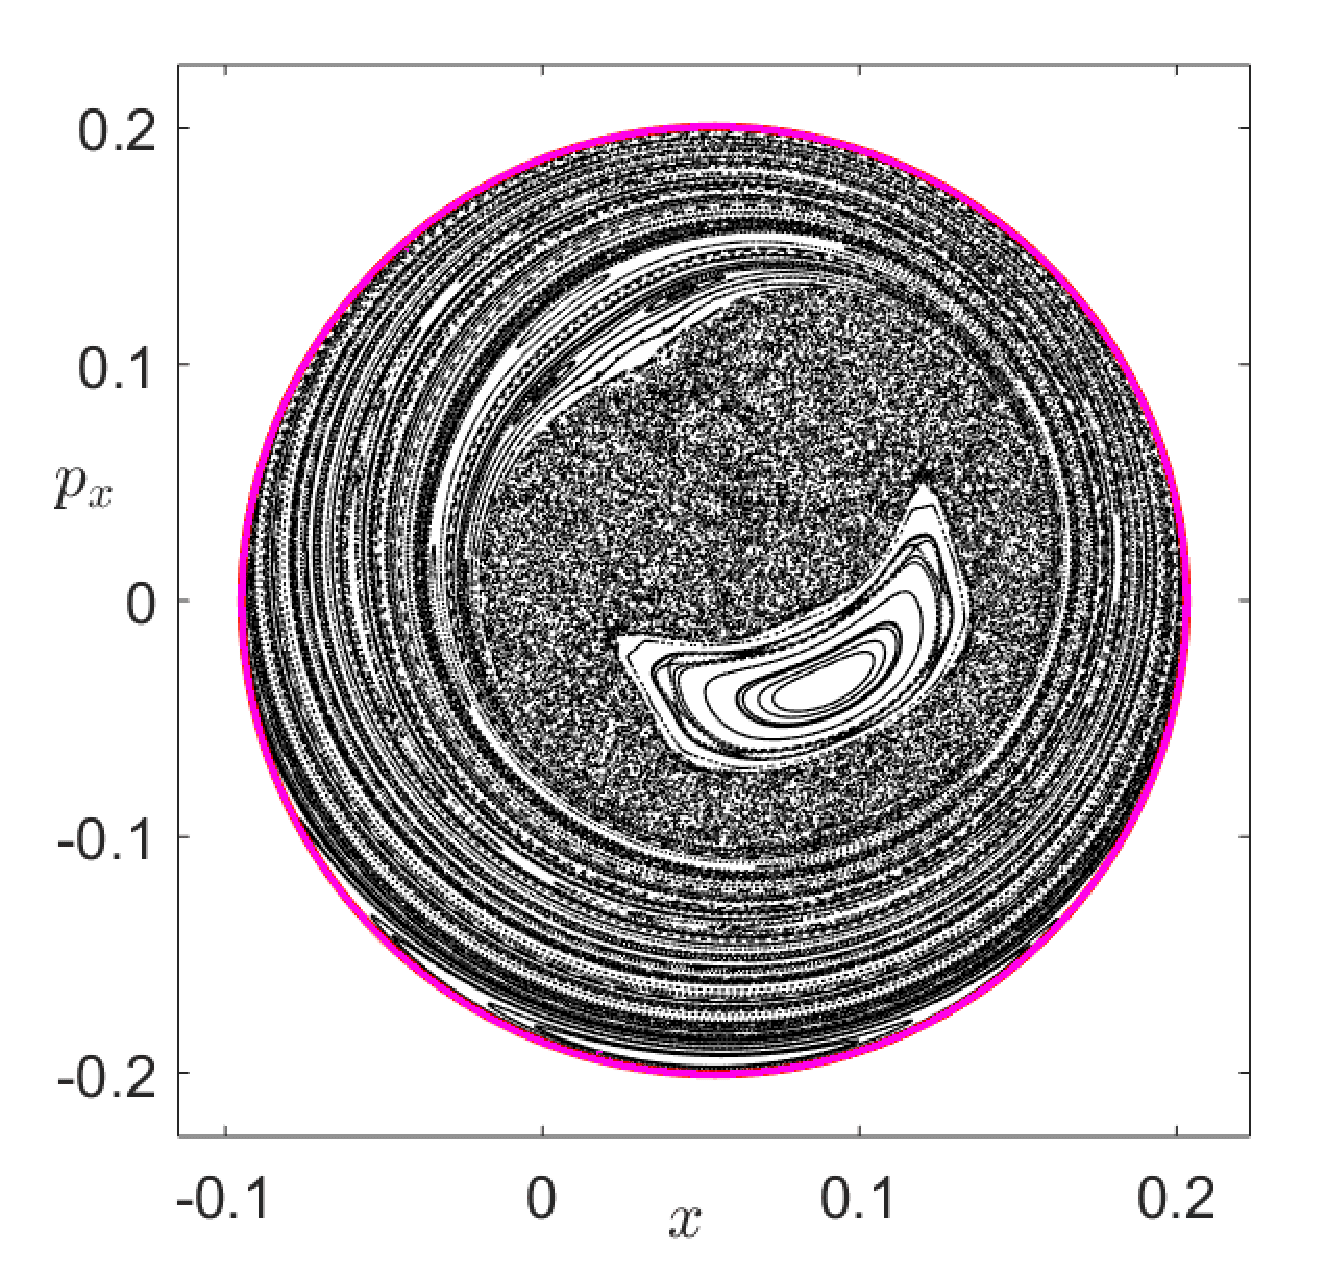
\includegraphics[scale=0.12]{fig10c.png}
		D)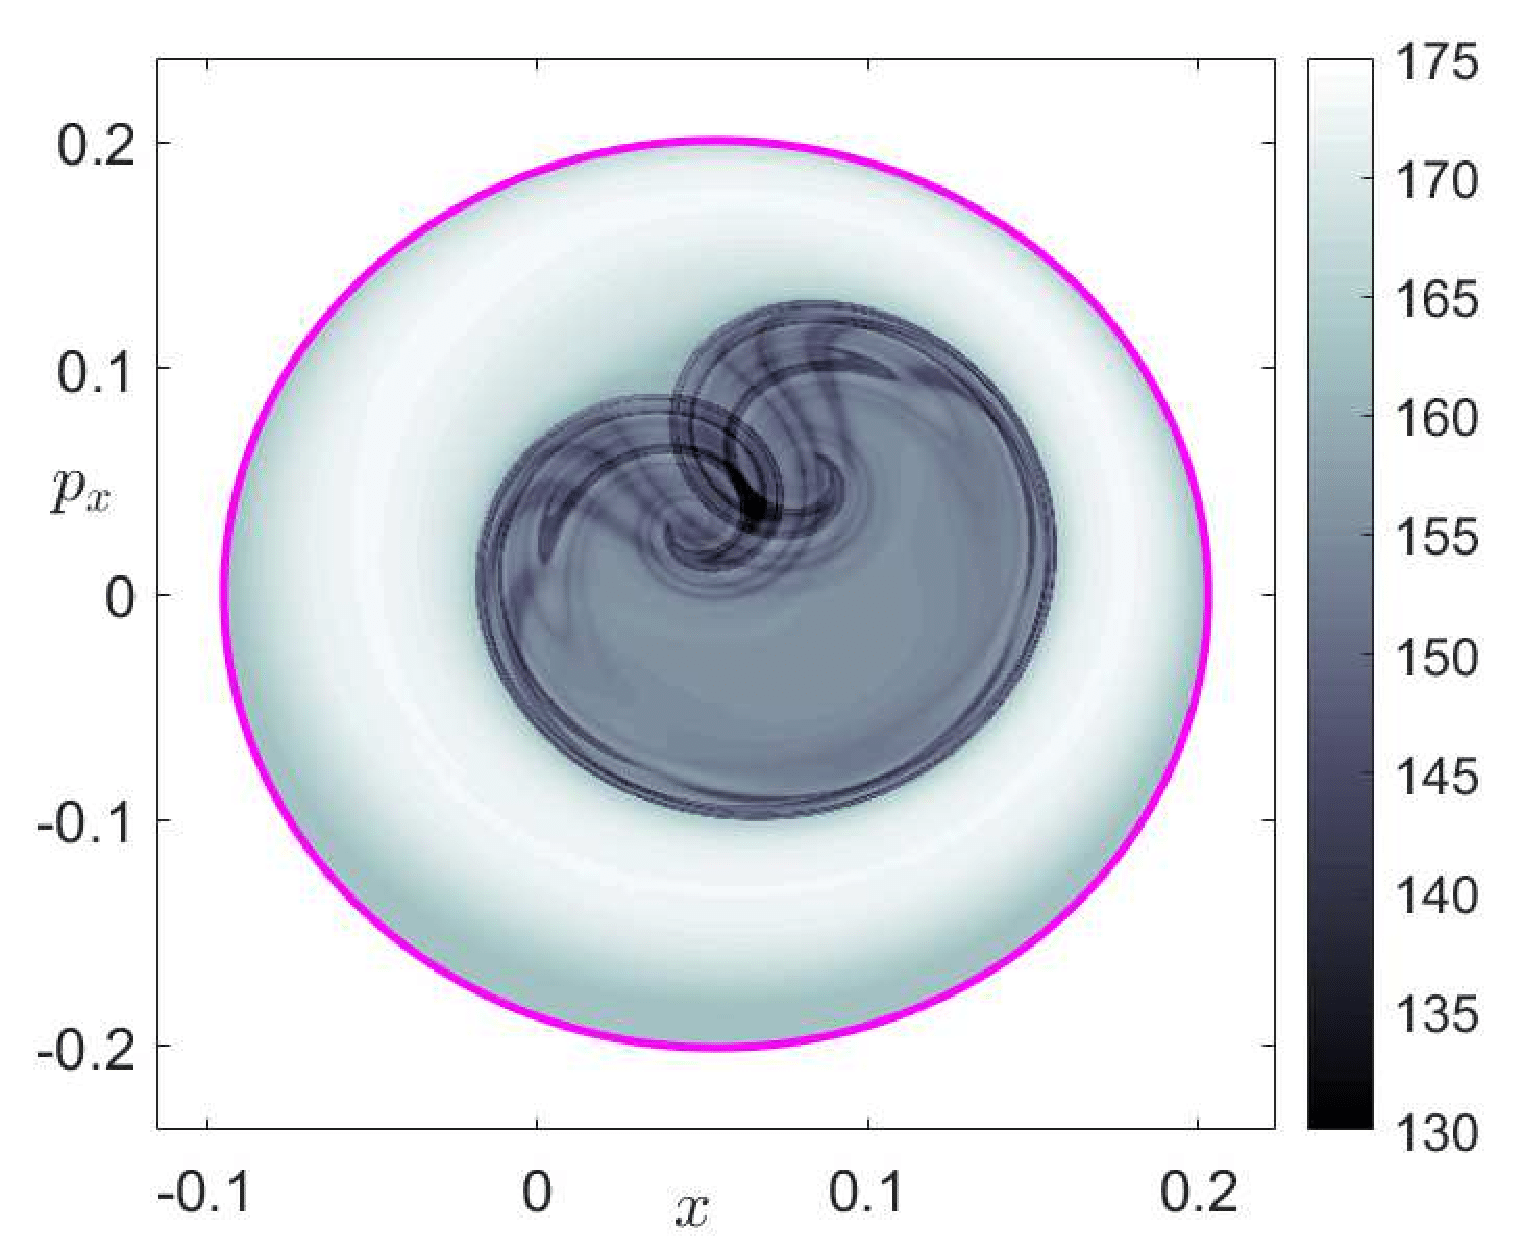
\includegraphics[scale=0.12]{fig10d.png}
	\end{center}
	\caption{Phase space structures of the coupled Hamiltonian with model parameters $\mu = 0.25$, $\alpha = 2$, $\omega = 1.25$ and $\varepsilon = 0.25$. The total energy of the system is $H_0 = 0$ (barrier energy). A) Poincar\'e map on the surface of section $\mathcal{U}^{+}_{qp}$; B) LDs calculated for $\tau = 75$ on the surface of section $\mathcal{U}^{+}_{qp}$; C) Poincar\'e map on the surface of section $\mathcal{U}^{+}_{xp_x}$; D) LDs calculated for $\tau = 75$ on the surface of section $\mathcal{U}^{+}_{xp_x}$. We have marked the energy boundary with a magenta curve.}
	\label{fig:ps_vs_ld_1}
\end{figure}

To finish the analysis, we consider the dynamics when the total energy is above that of the index-1 saddle, that is $H_0 > 0$, and in particular we will set $H_0 = 0.05$ in our computations. In this situation, a phase space bottleneck opens up in the barrier region, as shown in Fig. \ref{fig:EnergySurf_Hills}. In order to describe the structures that mediate reaction dynamics, that is the NHIM (or unstable periodic orbit) and its stable and unstable manifolds, we use differential correction and continuation along with globalization as described in \cite{Koon2011,naik2017geometry,naik2019b,GG2019}. In Fig. \ref{fig:set2_manifolds_upo_energysurf} panels C) and D), we show the cylindrical manifolds along with the energy surface and the unstable periodic orbit. In order to recover the homoclinic tangle geometry of the invariant manifolds, we calculate LDs on the surfaces of section $\mathcal{U}^{+}_{qp}$ and $\mathcal{U}^{+}_{xp_x}$, and compare with the direct numerical construction of these invariant manifolds. This LD based diagnostic is similar to performing a ``phase space tomography'' of the high dimensional phase space structures using a low dimensional slice. In Fig. \ref{fig:LD_NHIM_detect} we show the computation of variable time LDs for an integration time $\tau = 10$ on the slice $\mathcal{U}^{+}_{qp}$. We observe that Lagrangian descriptors clearly identify the location of the stable and unstable manifolds and the NHIM at the intersection of the invariant manifolds. Since we are using a small integration time of $\tau = 10$ to compute LDs, the complete geometry of the homoclinic tangle is not fully revealed. Therefore, in order to recover a more complete and intricate dynamical picture of the homoclinic tangle, the integration time to compute LDs has to be increased. This is shown in Fig. \ref{fig:ps_vs_ld_2}B), where $\tau = 30$ and we observe that the regular motion obtained in the middle of the Poincar\'e section displayed in Fig. \ref{fig:ps_vs_ld_2}A) corresponds to trajectories that remain trapped in the potential well region and never escape. The trapped dynamics on the tori are also captured by the LD contour map shown in Fig. \ref{fig:ps_vs_ld_2}B) which also reveals the homoclinic tangle of the stable and unstable manifolds and the resulting lobe dynamics \cite{beigie1992}. We note that in all these computations we are using the variable time definition of LDs, since the open potential surface causes trajectories to escape to infinity through the bottleneck in finite time, resulting in NaN values in the LD contour map and would hide the important underlying phase space structures making the interpretation of results difficult. In addition, when we analyze the dynamics using Poincar\'e sections, we cannot ensure that trajectories return to the surface of section when the dynamical behavior of escaping to infinity is possible in the system. This will result in blank regions in the Poincar\'e sections as shown in Fig. \ref{fig:ps_vs_ld_2}A) and C). However, we note that trapped trajectories in the potential well corresponding to regular (motion on the tori) and chaotic motion are highlighted as expected in the Poincar\'e sections. These trajectories are non-reactive and will remain so until they satisfy the \textit{sufficient} condition for reaction which is entering the cylindrical manifolds. 

\begin{figure}[!ht]
	\begin{center}		
	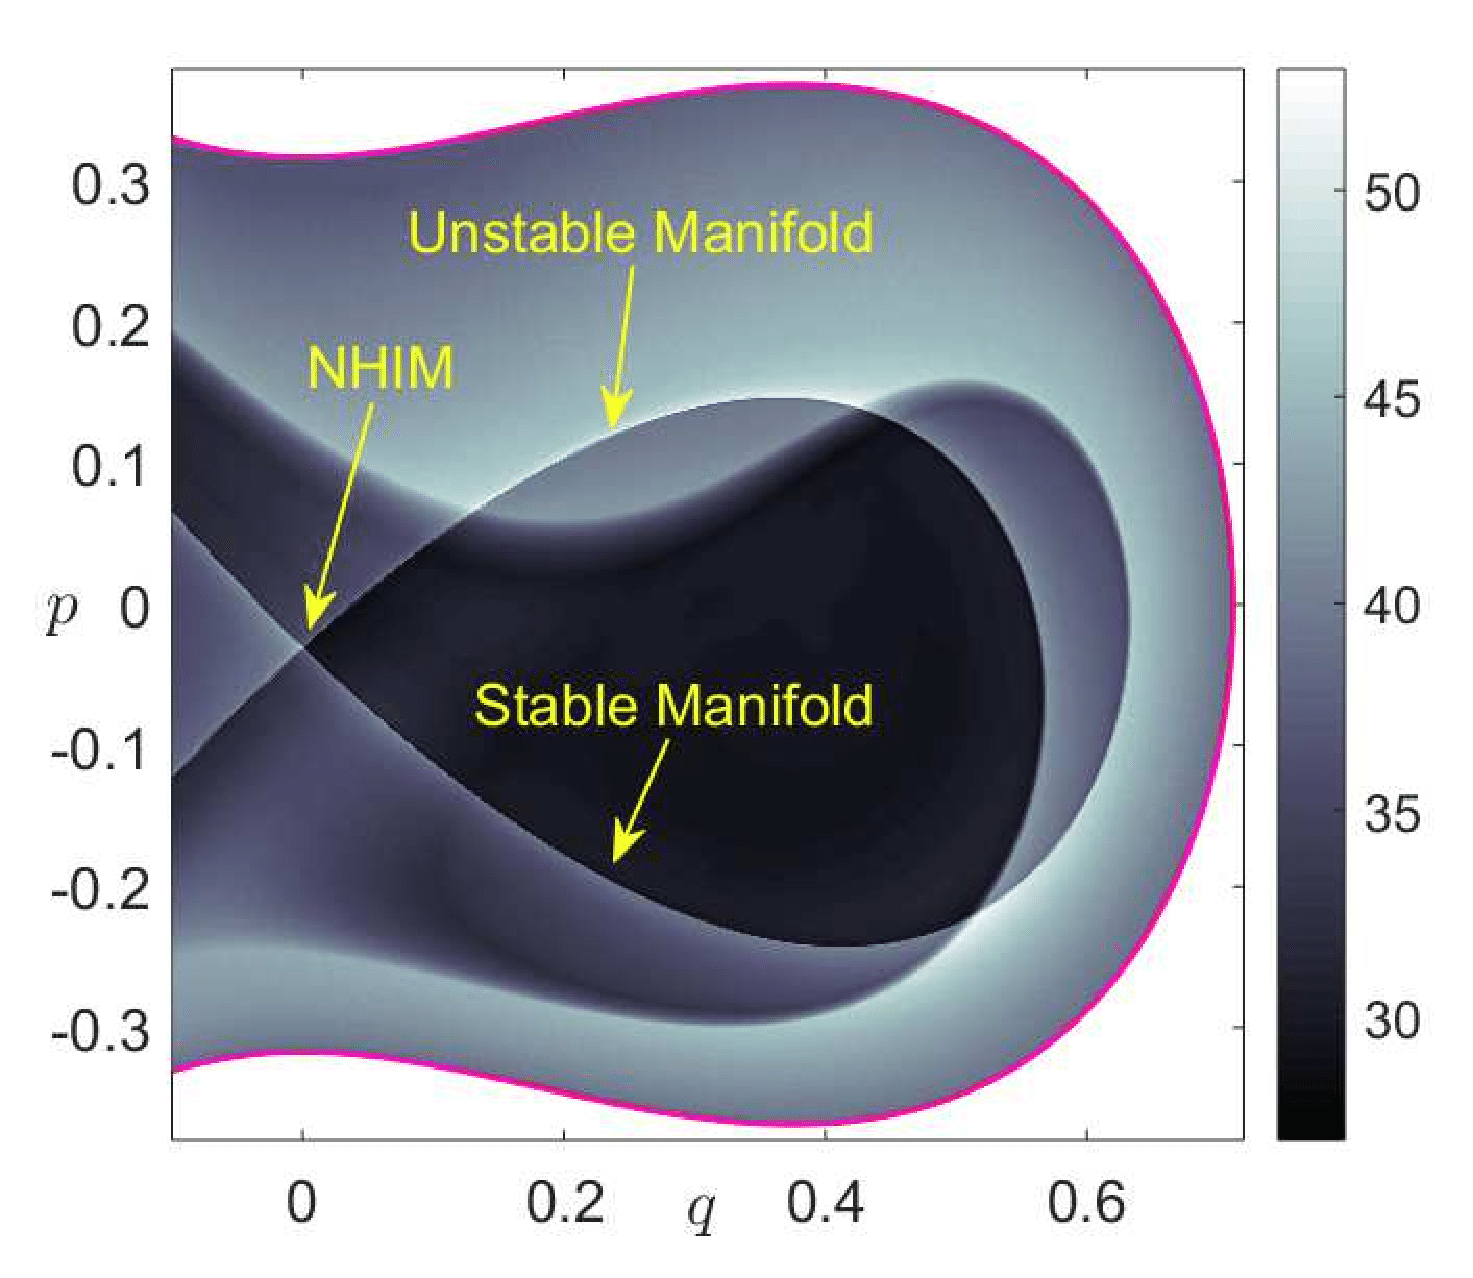
\includegraphics[scale=0.14]{fig11.png}
	\end{center}
	\caption{Variable time LDs calculated on the surface of section $\mathcal{U}^{+}_{qp}$ for $\tau = 10$. The NHIM and its stable and unstable manifolds are revealed as points where the LD field in non-differentiable and attains a local minimum. We have marked the energy boundary with a magenta curve.}
	\label{fig:LD_NHIM_detect}
\end{figure}

Identifying the regions inside the cylindrical (tube) stable and unstable manifolds can be done using globalization or using the LD contour map on appropriate isoenergetic surfaces. We compute LD contour maps to recover the intersections of these tube manifolds with the surface of section in Eq. \eqref{eq:sos_xpx}. The intersection of the invariant manifolds with the isoenergetic surface of section yields topological ellipses, known in the chemical reactions literature as \textit{reactive islands} \cite{deleon1991a,deleon1991b,deleon1992,patra2018detecting} which are of paramount importance for the computation of reaction rates/fraction. In order to illustrate the capability of LDs to recover the reactive island structure, we have compared the LD contour map and manifold intersection with the surface of section $\mathcal{U}^{+}_{xp_x}$ obtained using globalization in Fig. \ref{fig:LD_Manifolds}. We have shown the first intersection of the stable and unstable manifolds with the surface of section as a blue/red curve superimposed on the LD contour map. We observe that the points at which the LDs scalar field is non-differentiable and the manifolds intersections are in agreement, thus verifying the LD based identification of reactive islands. We also observe that successive folds and resulting intersections of the tube manifolds with the surface of section are also revealed by LDs. We note here that the first intersection of the manifolds encloses a large phase space volume in the potential well which indicates that a large portion of the potential well escapes to infinity through the bottleneck. This is despite the fact that we have chosen a very small value for the energy of the system, $H_0 = 0.05$, compared to the energy of the barrier. This is a consequence of using a high coupling strength, $\varepsilon = 0.25$, which makes the vase-like shaped potential well region small and narrow, since the center equilibrium point at the bottom of the potential well approaches the index-1 saddle equilibrium point at the origin as $\varepsilon$ is increased. Movies illustrating the change in both the shape of the energy surface and the equipotentials in configurations space as we vary the coupling strength can be found at the links https://youtu.be/kYklCrSwtls and https://youtu.be/0FNChWVM6nU respectively. We can see that the effect of increasing the coupling strength from zero is to \textit{tilt and squeeze} the vase-like shape of the energy surface that qualitatively increases the number of reactive trajectories. This action of tilting and squeezing of the vase-like container (boundary defined by the total energy surface) is to pour out its contents (the reactive trajectories) and hence the increase in reaction fraction. A quantitative investigation of this phenomenon is current work in progress and beyond the scope of this chapter.

\begin{figure}[!ht]
	\begin{center}		
		A)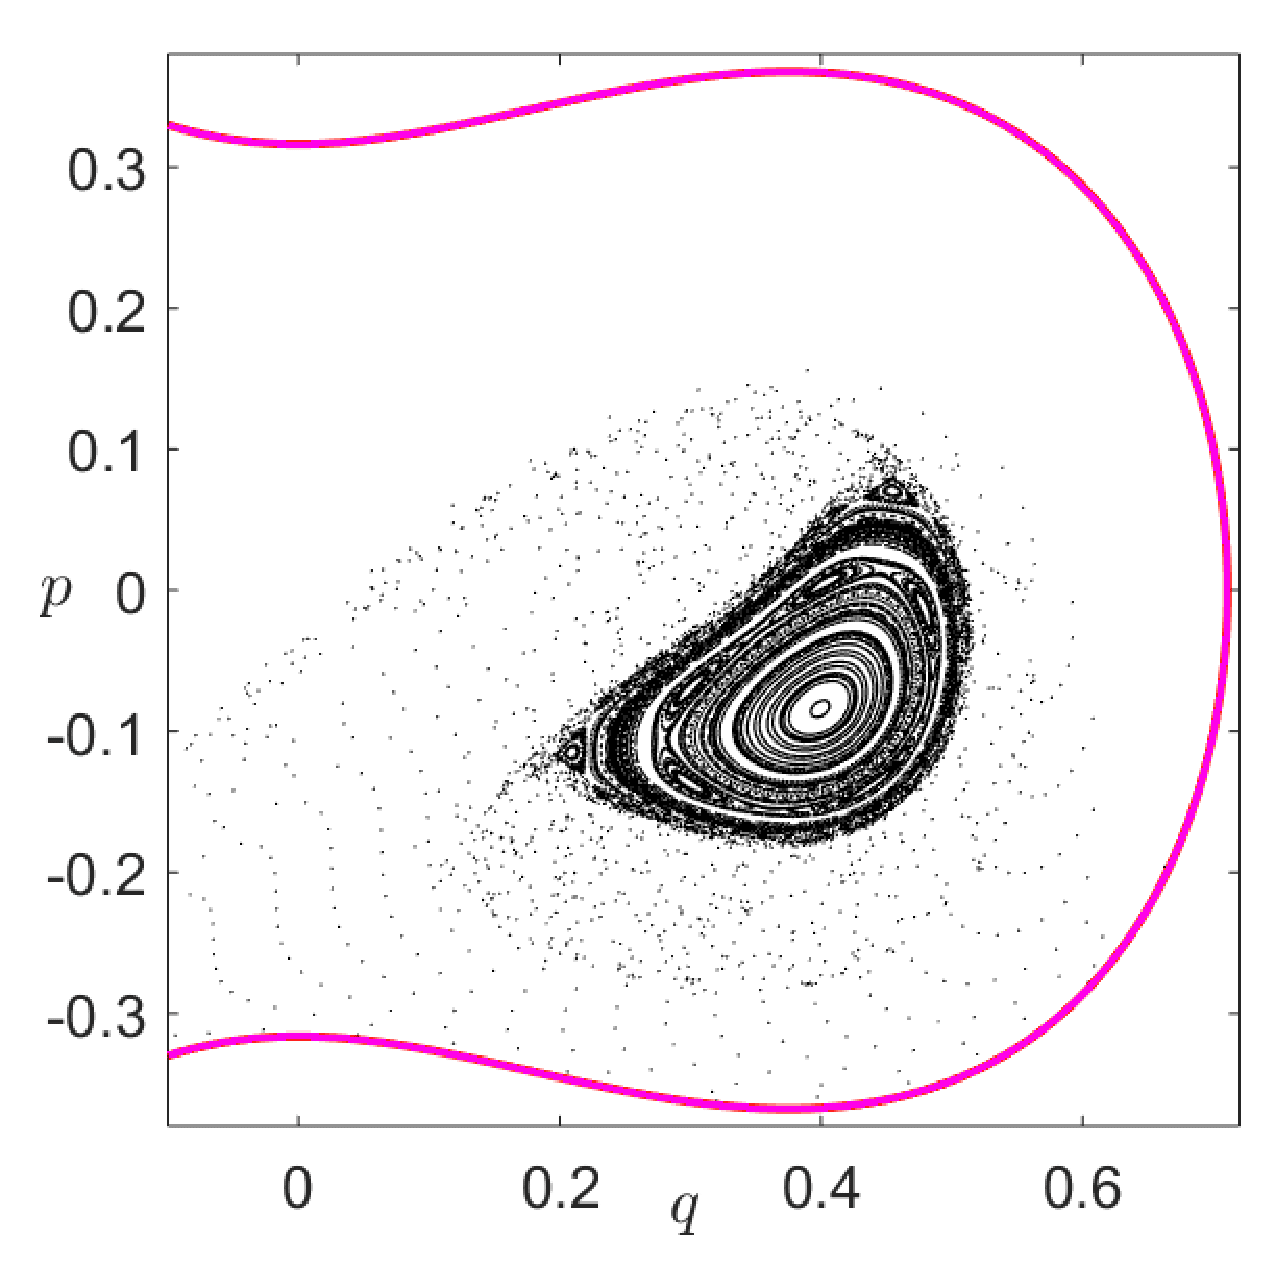
\includegraphics[scale=0.12]{fig12a.png}
		B)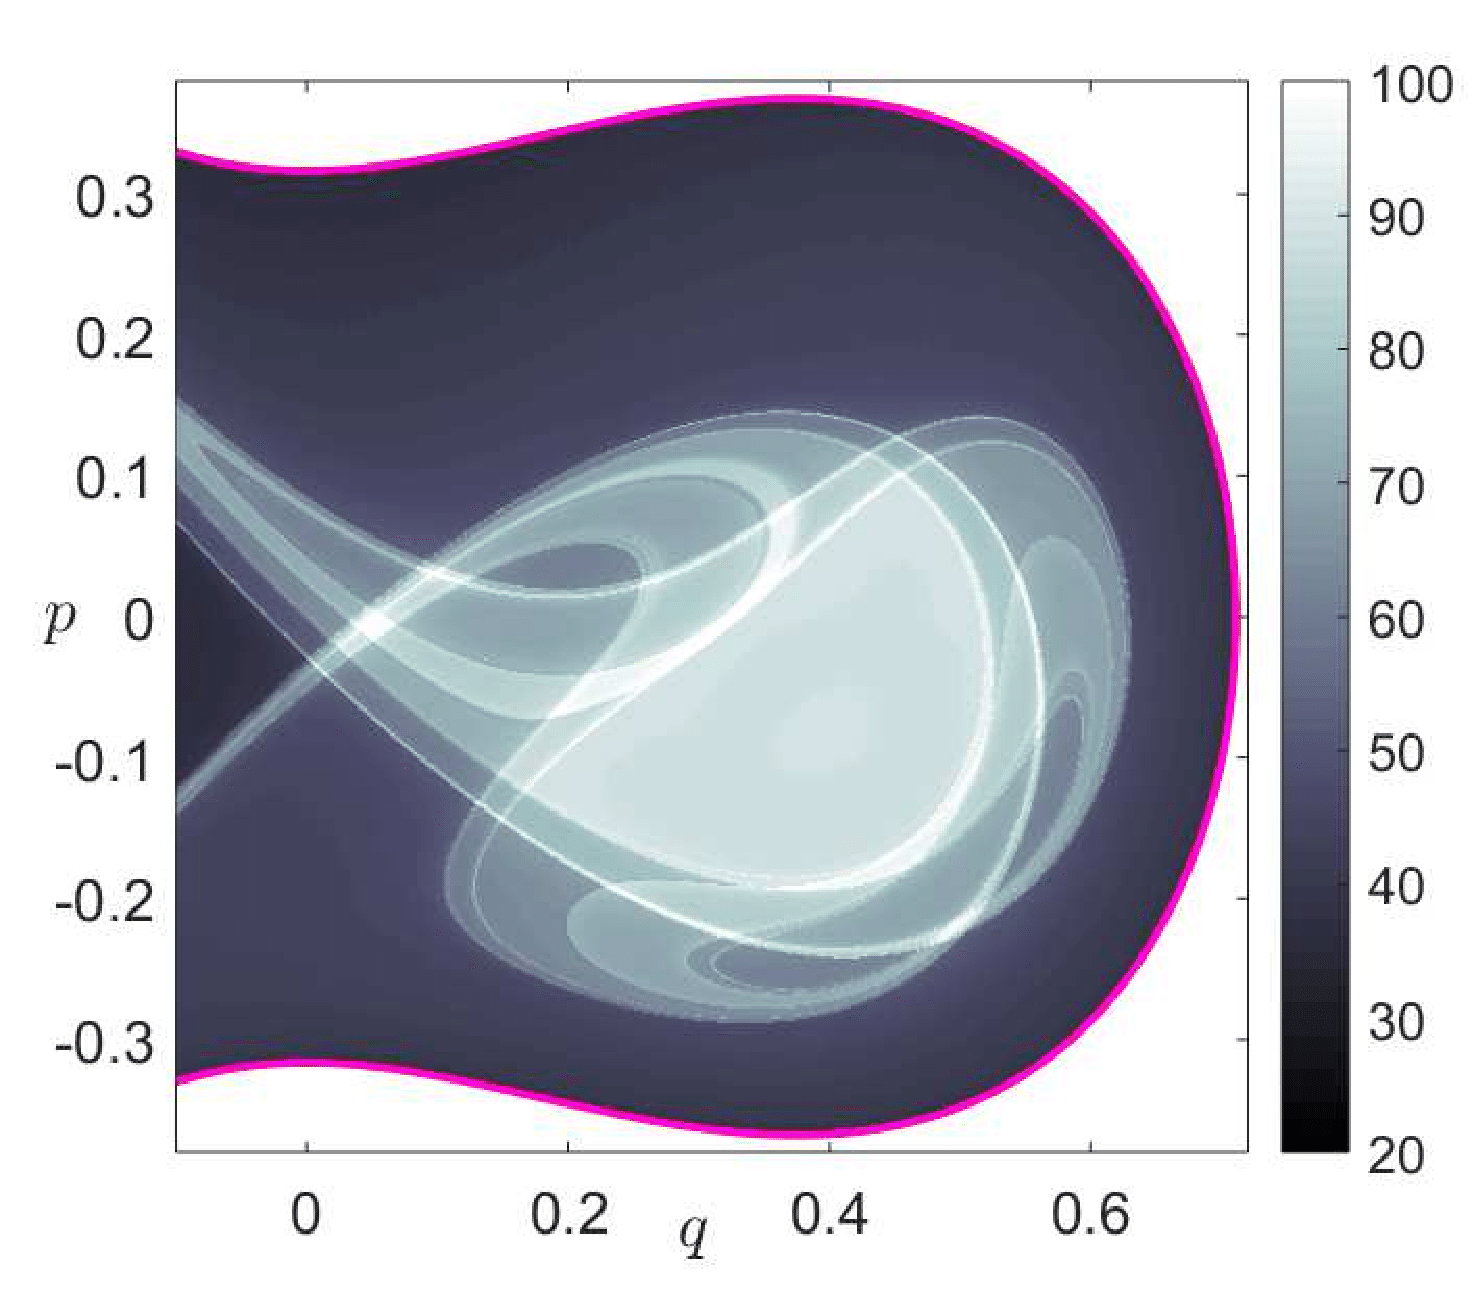
\includegraphics[scale=0.12]{fig12b.png}
		C)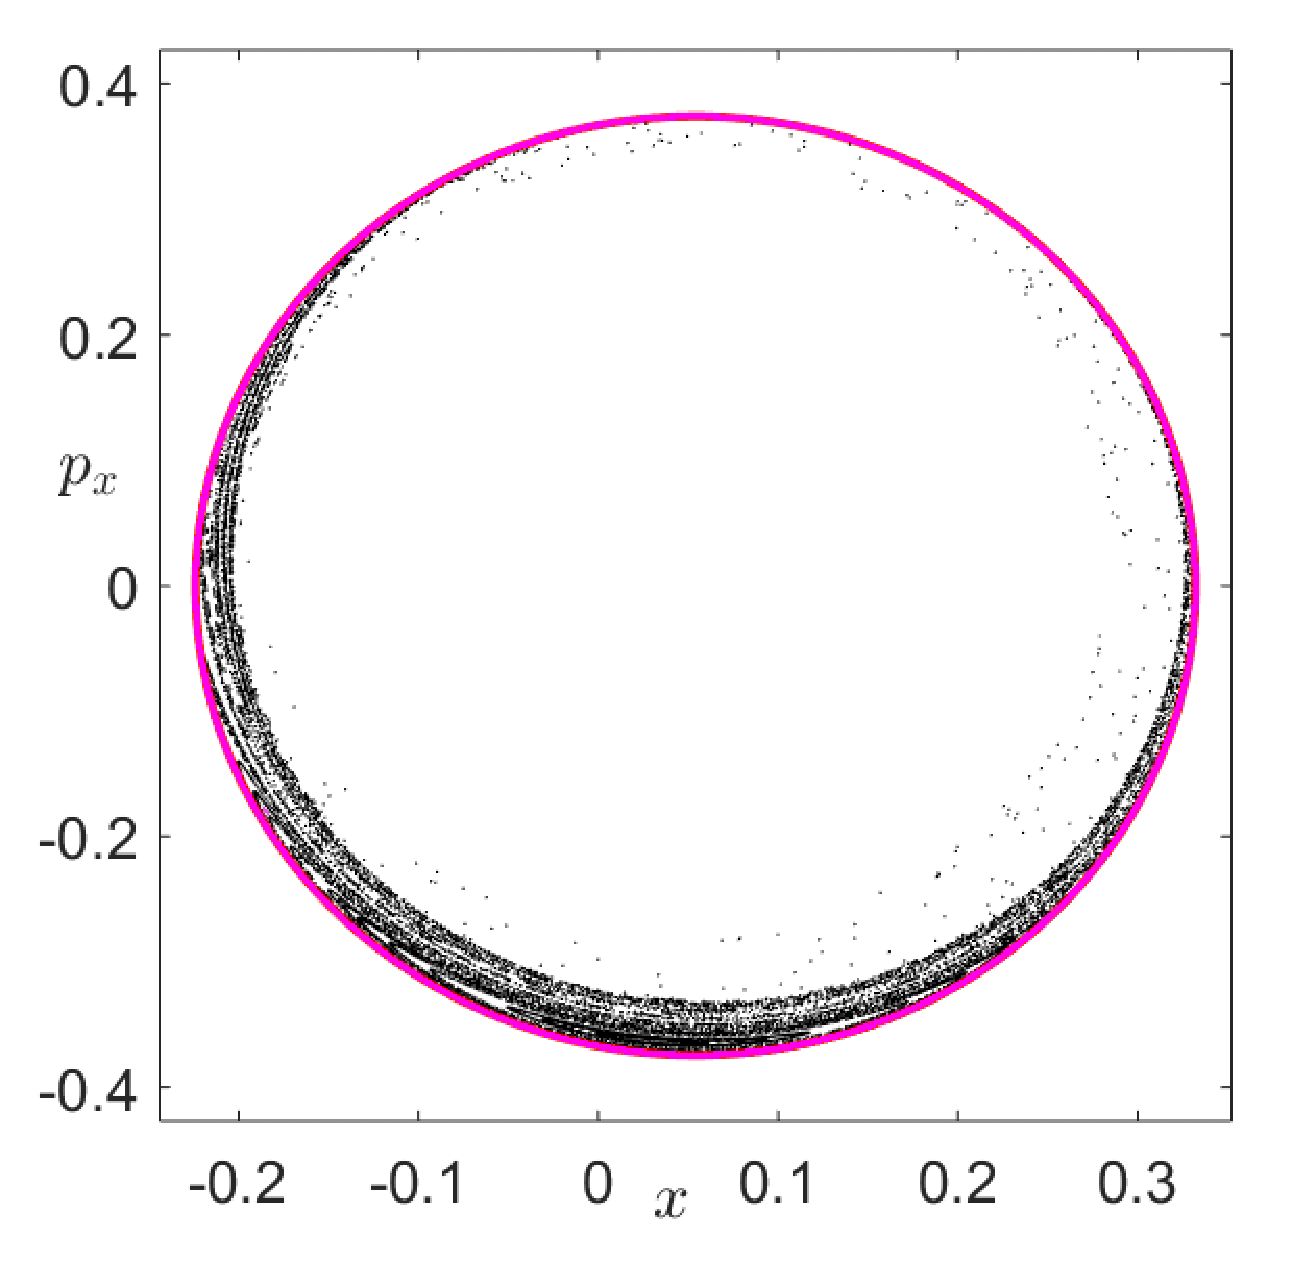
\includegraphics[scale=0.12]{fig12c.png}
		D)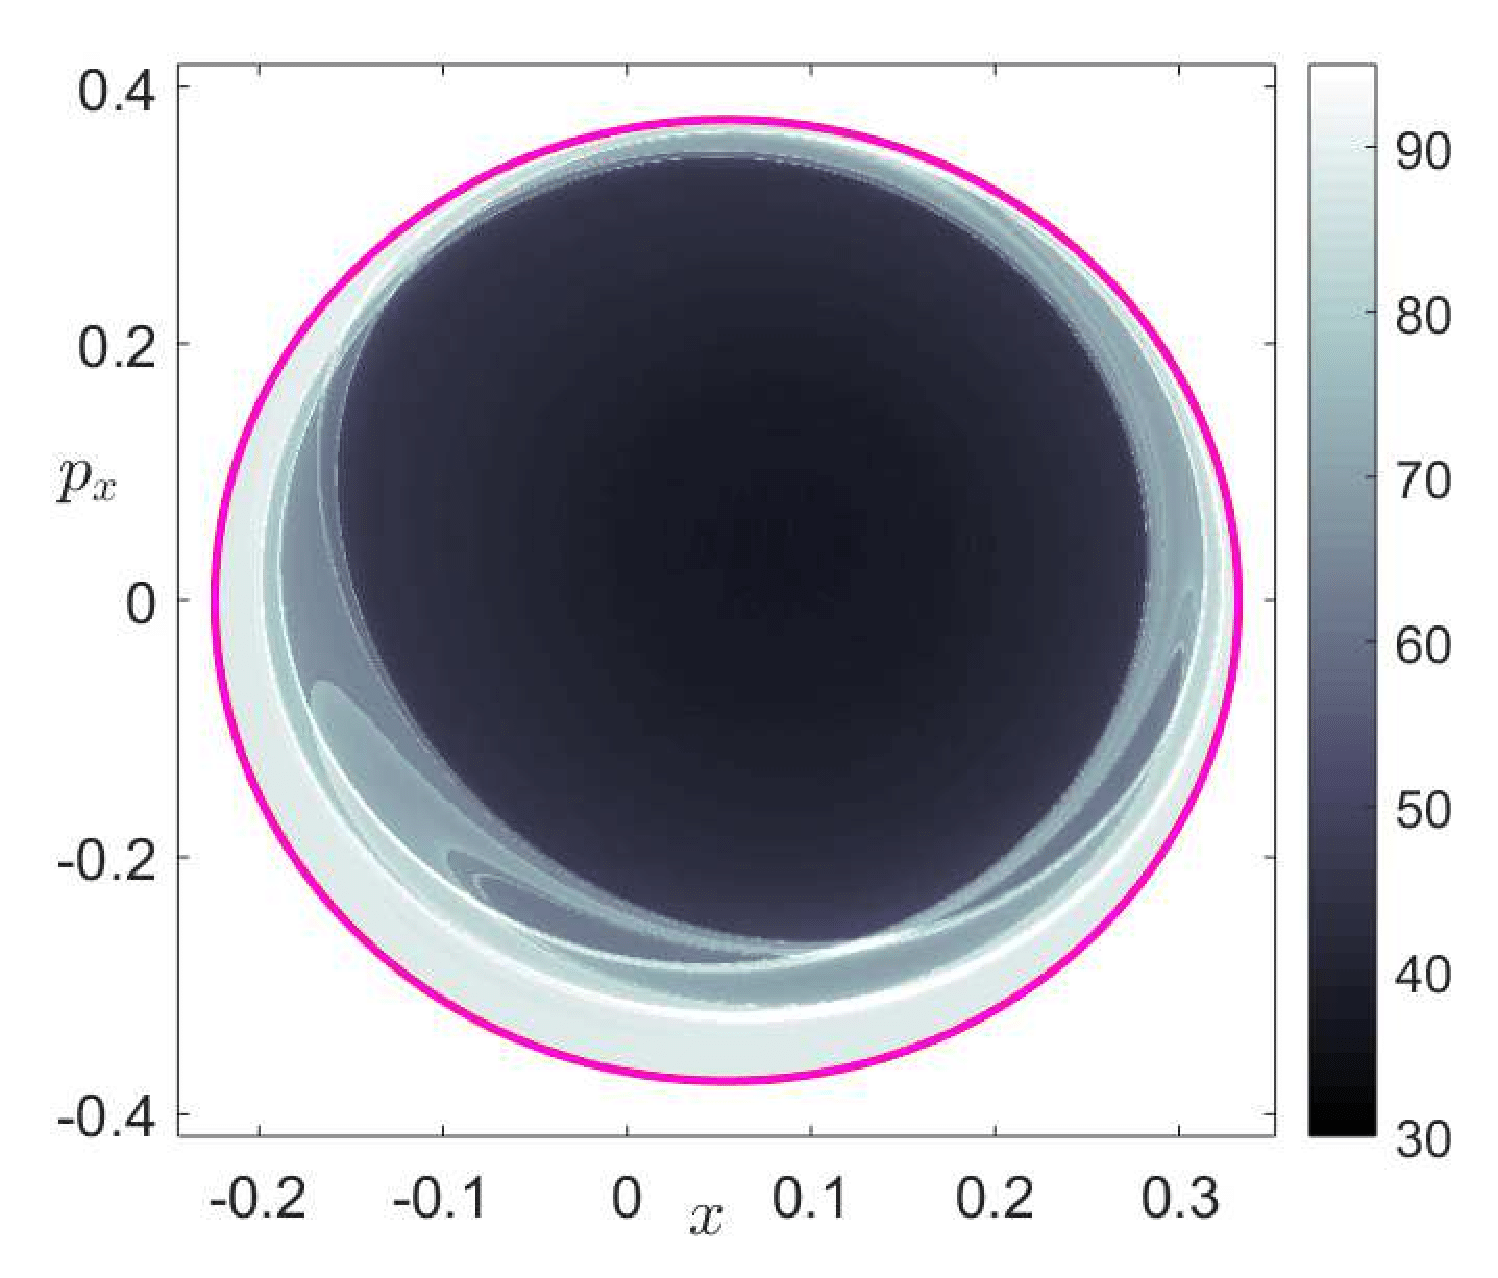
\includegraphics[scale=0.12]{fig12d.png}
	\end{center}	
	\caption{Phase space structures of the coupled Hamiltonian with model parameters $\mu = 0.25$, $\alpha = 2$, $\omega = 1.25$ and $\varepsilon = 0.25$. The total energy of the system is $H_0 = 0.05$,	which is above the barrier energy. A) Poincar\'e map on the surface of section $\mathcal{U}^{+}_{qp}$; B) LDs calculated for $\tau = 30$ on the surface of section $\mathcal{U}^{+}_{qp}$; C) Poincar\'e map on the surface of section $\mathcal{U}^{+}_{xp_x}$; D) LDs calculated for $\tau = 30$ on the surface of section $\mathcal{U}^{+}_{xp_x}$. We have marked with a magenta curve the energy boundary.}
	\label{fig:ps_vs_ld_2}
\end{figure}

\begin{figure}[htbp]
	\begin{center}		
		A)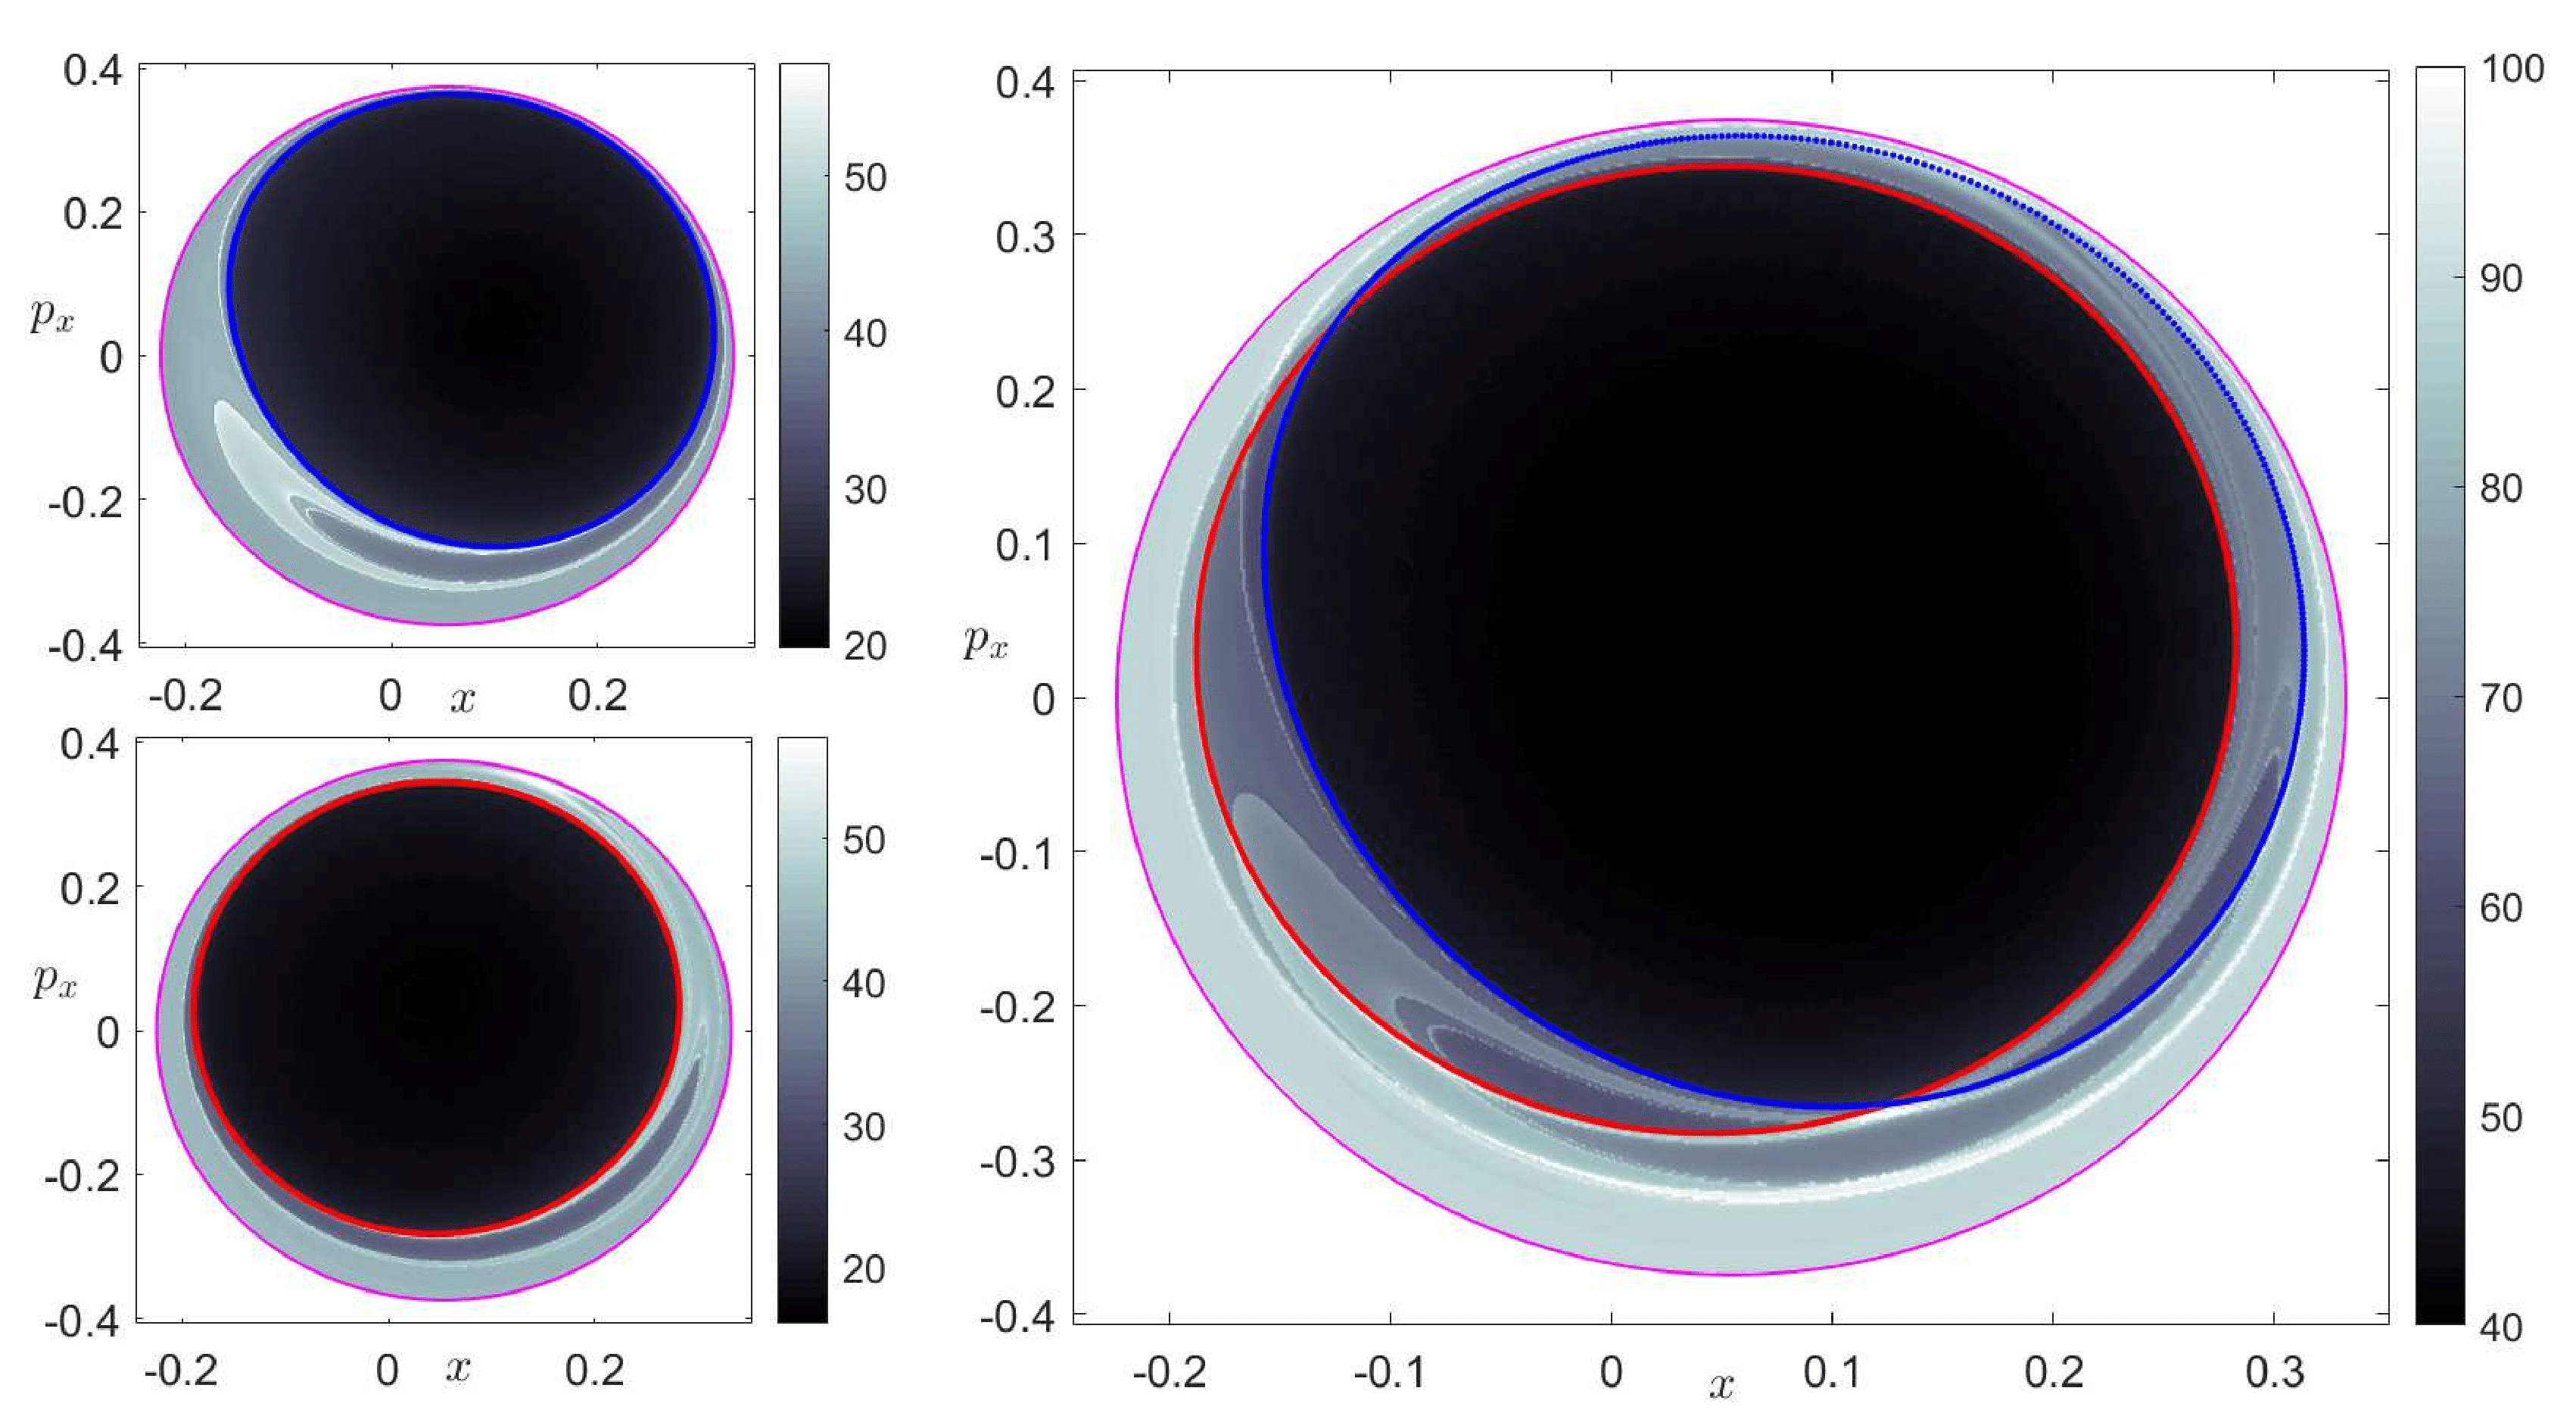
\includegraphics[scale=0.102]{fig13a.png}
		B)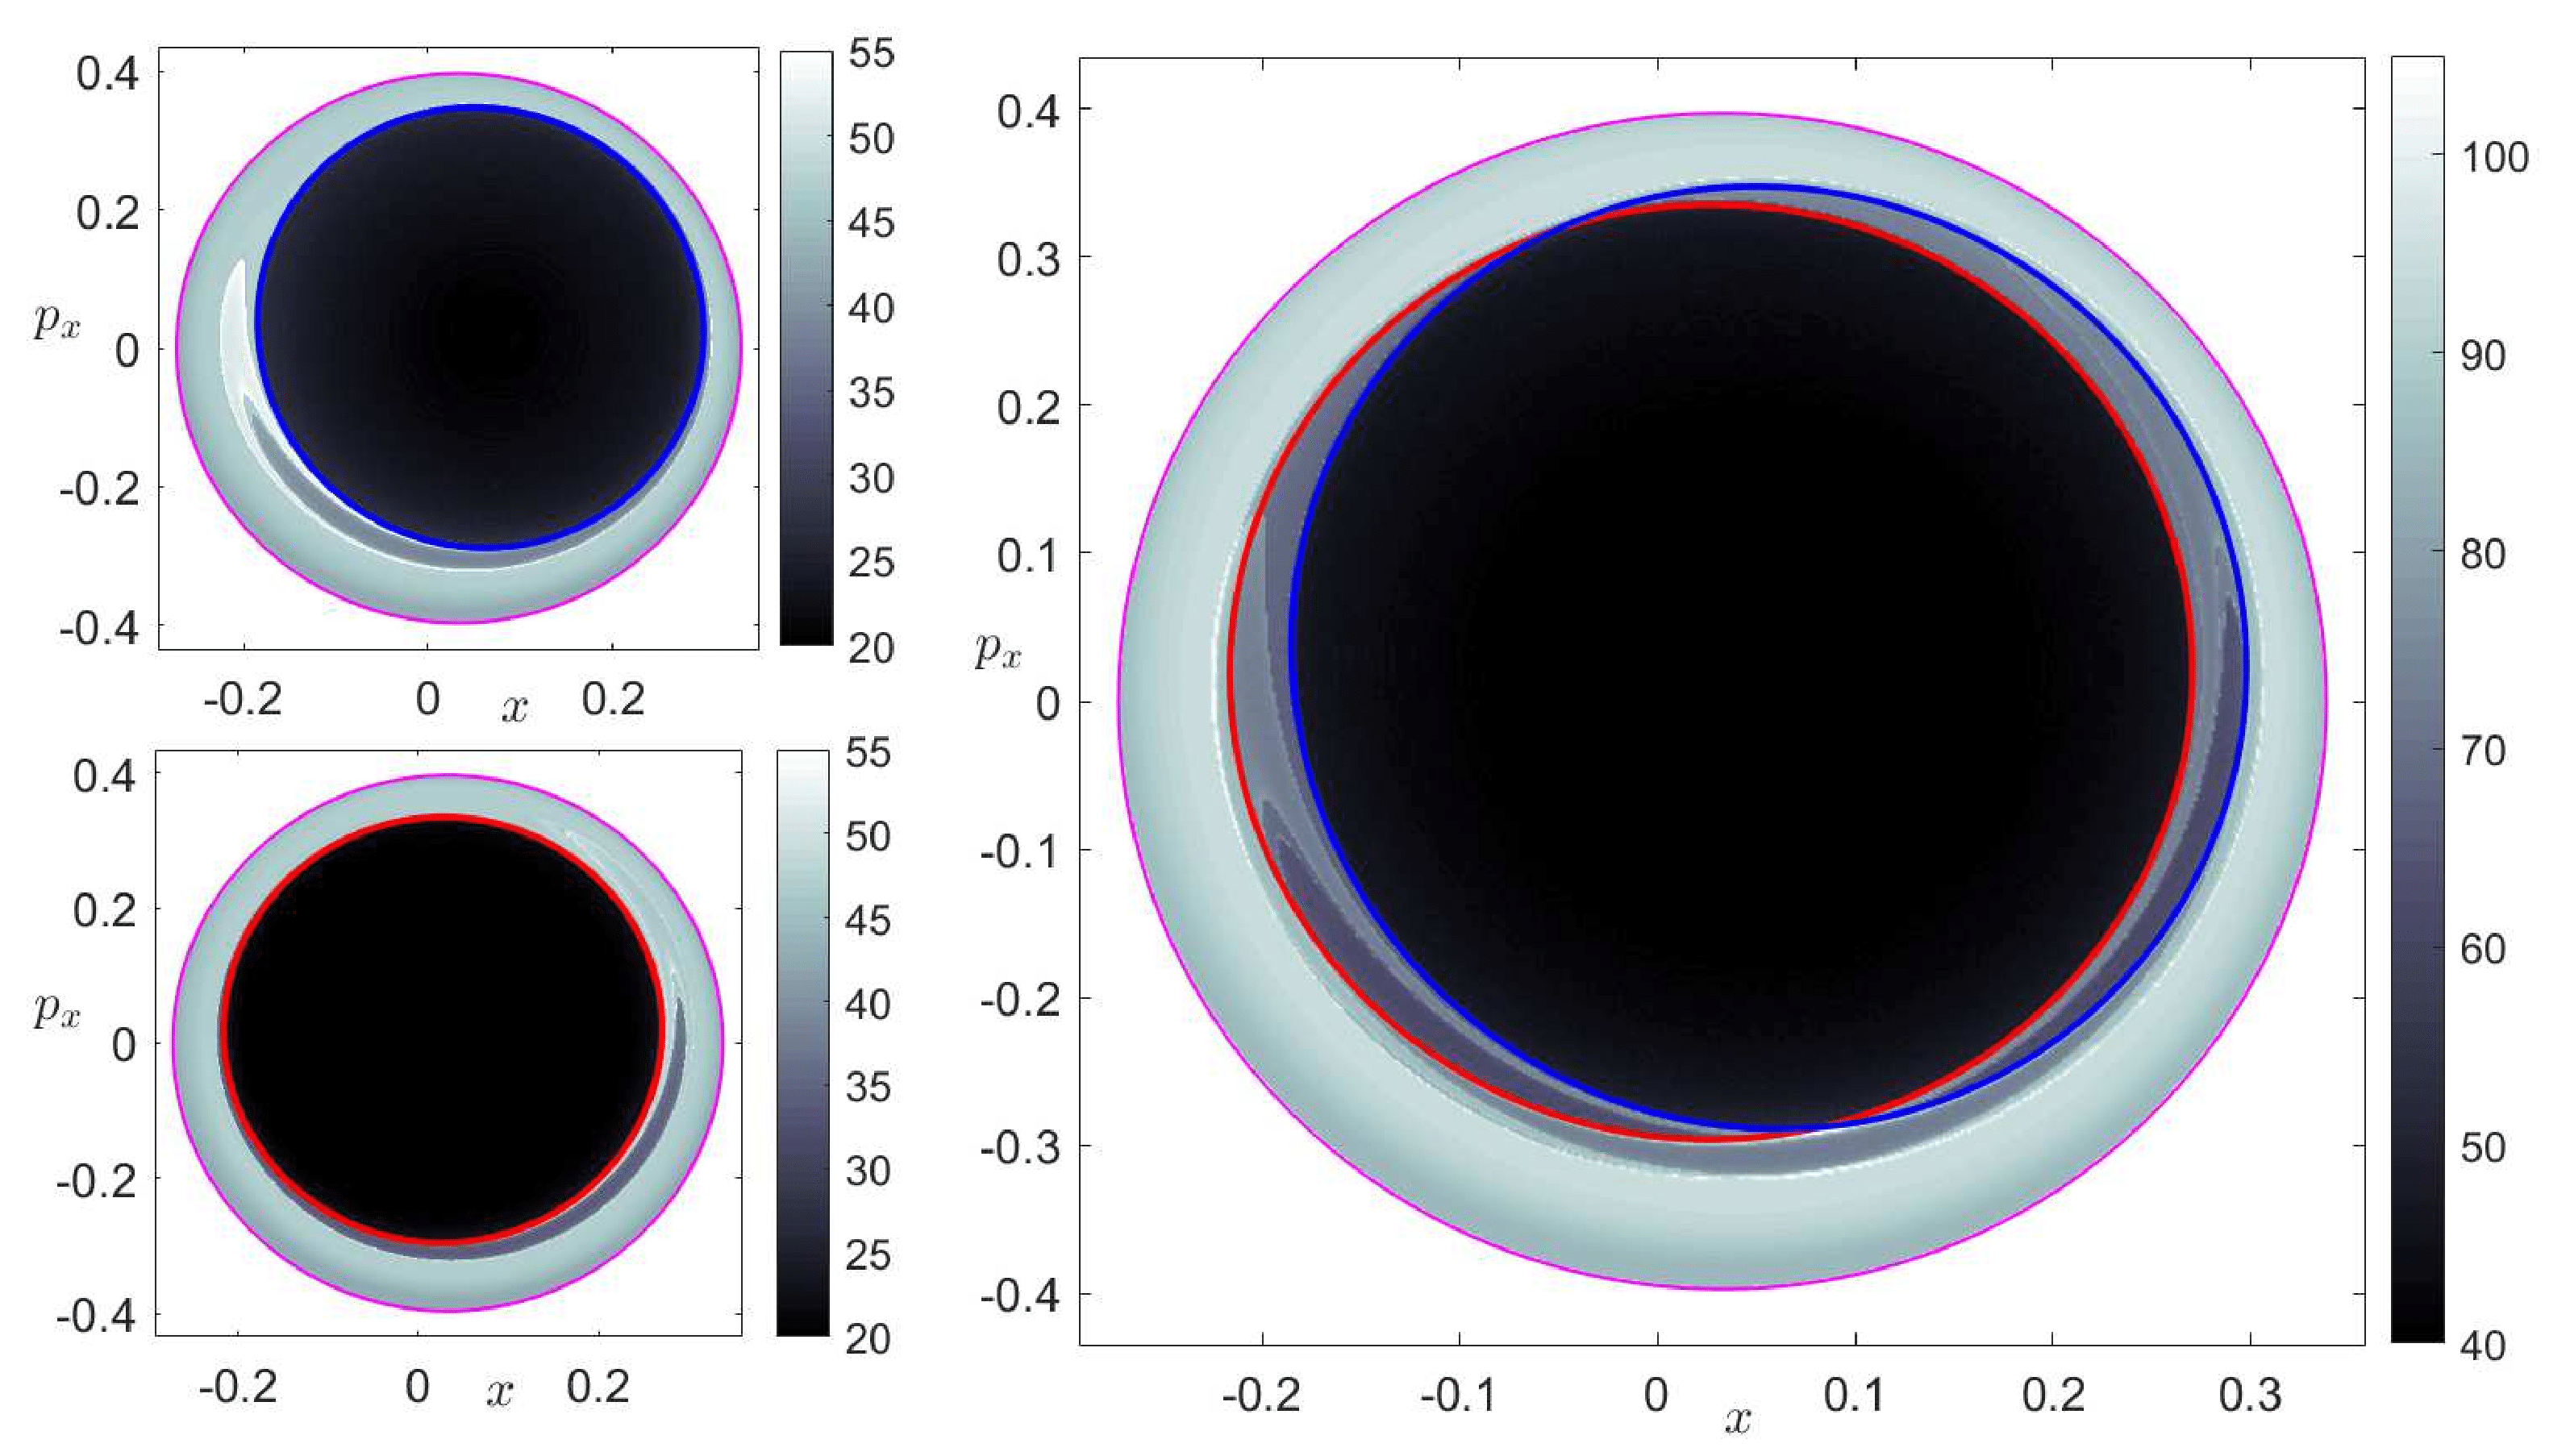
\includegraphics[scale=0.11]{fig13b.png}
	\end{center}
	\caption{Phase space structures revealed by LDs using $\tau = 30$ for the coupled Hamiltonian with parameters $\mu = 0.25$, $\alpha = 2$, $\omega = 1.25$ and total energy $H_0 = 0.05$. A) Coupling strength $\varepsilon = 0.25$. On the top/bottom left we show the forward/backward LD and, superimposed, the first intersection of the stable/unstable manifold with $\mathcal{U}^{+}_{xp_x}$ as a blue/red curve. On the right, the total LD is depicted (addition of forward and backward LD) together with the first intersection of the stable and unstable manifolds. The magenta curve represents the energy boundary. B) same analysis using $\varepsilon = 0.125$.}
	\label{fig:LD_Manifolds}
\end{figure}

\bibliography{HamSN}

\end{document}